\documentclass{report}
\usepackage[utf8]{inputenc}
\usepackage{amsmath}
\usepackage{amsfonts}
\usepackage{hyperref}
\usepackage{tcolorbox}
\usepackage{breqn}
\usepackage{adjustbox}
\usepackage{changepage}
\usepackage{rotating}
\usepackage{algorithm}
\usepackage{algpseudocode}
\usepackage{ntheorem}

% Definition
\newtheorem{definition}{Definition}{\bfseries}{\itshape}
\newtheorem*{definition*}{Definition}{\bfseries}{\itshape}

% Theorem
\newtheorem{theorem}{Theorem}{\bfseries}{\itshape}

% Concept
\newtheorem*{concept}{}{\bfseries}{\itshape}

\title{Analysis of the diffusion property in DES, AES and SAFER $S$-Boxes}
\author{Ana Clara Zoppi Serpa\\ Prof. Dr. Ricardo Dahab \\ Dr. Jorge Nakahara Jr.}
\date{\today}

\begin{document}

\maketitle

\chapter{Analysis of the diffusion property in the DES, AES and SAFER $S$-Boxes}
In this chapter, we obtain the Algebraic Normal Forms (ANFs) of the $S$-Boxes (Substitution Boxes) of three ciphers (DES \cite{DES-FIPS}, AES \cite{AES-FIPS} and SAFER \cite{SAFER-1993}), and use them to analyze and compare these $S$-Boxes with respect to the complete diffusion (see Definition \ref{def:complete-diffusion}) cryptographic property.

We assume the reader is familiar with the following concepts:
\begin{itemize}
    \item the XOR Boolean function (see Chapter \textcolor{red}{X}),
    \item block ciphers (see Chapter \textcolor{red}{X}),
    \item vectors and vector spaces (see Chapter \textcolor{red}{X}),
    \item the AES cipher (see Chapter \textcolor{red}{X}),
    \item the DES cipher (see Chapter \textcolor{red}{X}),
    \item the SAFER cipher (see Chapter \textcolor{red}{X}).
\end{itemize}

\section{Notation}
\begin{itemize}
    \item $\mathbb{F}_2$: the finite field $\{0, 1\}$, also denoted by $GF(2)$ in the literature
    \item $\mathbb{F}^n_2$, $\mathbb{F}^m_2$: vector spaces of dimension $n$ ($m$) with elements of $\mathbb{F}_2$, i.e ``bit vectors"
    \item $n$: dimension of a vector space, also, the number of variables (inputs) of a vectorial Boolean function ($S$-Box)
    \item $m$: dimension of a vector space, also, the number of outputs of a vectorial Boolean function ($S$-Box)
    \item $f$: a Boolean function
    \item $x_i$: an input variable of a Boolean function
    \item $x$: ordered tuple $(x_1, ..., x_n)$ with the inputs of a Boolean function
    \item $u, x$: monomials of the Algebraic Normal Form of a Boolean function
    \item $a_i$: a coefficient of the Algebraic Normal Form of a Boolean function
    \item $y_i$: an output bit of a vectorial Boolean function
    \item $y$: ordered tuple $(y_1, ..., y_m)$ with the outputs of a vectorial Boolean function
    \item $x_ix_j$: multiplication of $x_i$ and $x_j$ in $\mathbb{F}_2$, i.e $x_i \cdot x_j$, in all the ANFs presented in this chapter
    \item $S_1, S_2, S_3, S_4, S_5, S_6, S_7, S_8$: $S$-Boxes of the DES algorithm
\end{itemize}

\section{Acronyms}
\begin{itemize}
    \item ANF: Algebraic Normal Form of a Boolean function
    \item $S$-Box: Substitution Box
    \item DES: Data Encryption Standard
    \item AES: Advanced Encryption Standard
    \item SAFER: Secure And Fast Encryption Routine
\end{itemize}

\section{Preliminaries}\label{sec:preliminaries}
Claude Shannon introduced, in \cite{Shannon1949}, two concepts that became essential for the design of secure ciphers: \emph{confusion} and \emph{diffusion}. He addresses these concepts considering the encryption of English texts, thus, in his paper, the plaintext and ciphertext symbols are the alphabet letters. However, we can easily adjust the concepts to discuss relationships between bits instead of relationships between letters, since any information is represented by bits in a computer, or, formally, by elements of the finite field $\mathbb{F}_2 = \{0,1\}$.

\begin{concept}[Confusion]
Refers to how ciphertext bits relate to plaintext (key) bits. The relationship must be complex, so that it is computationally unfeasible to be exploited in an attack.
\end{concept}

\begin{concept}[Diffusion]
Refers to the influence of each plaintext (key) bit upon the ciphertext bits. This influence must be as widespread as possible.
\end{concept}

These two properties are extremely relevant for the design of modern ciphers --- all of them must strive for confusion and diffusion of plaintext and key bits. Actually, all modern ciphers should achieve \emph{complete diffusion} (see Definition \ref{def:complete-diffusion}) in order to be secure. Modern block ciphers particularly achieve this through iterations, substitutions, linear operations and permutations.

It's relevant to note that complete diffusion should be achieved (and evaluated whilst designing a cipher) for both plaintext and key, although in this chapter we analyze only plaintext diffusion.

\begin{definition}[Complete Diffusion]\label{def:complete-diffusion}
When each ciphertext bit depends on all plaintext (key) bits, complete diffusion has been achieved by the cipher.
\end{definition}

An $S$-Box (Substitution Box) is a component, commonly used by block ciphers, to achieve confusion and diffusion. $S$-Box usage was introduced by Feistel \cite{Feistel1973}. Furthermore, \cite{Feistel1973} proposes that $S$-Boxes and permutations be combined in order to build strong ciphers, i.e they ``work together", playing central roles towards ensuring confusion and diffusion. In other words, using only $S$-Boxes does not provide complete diffusion/confusion. Similarly, using only permutations would not attain complete diffusion/confusion either. Both components are relevant for the overall security of the cipher with respect to these properties.

\begin{concept}[$S$-Box]
An $S$-Box (Substitution Box) is a non-linear mapping from an $n$-bit vector to an $m$-bit vector, usually implemented as lookup table.
\end{concept}

In the case of DES, for instance, the $S$-Boxes are presented as integer-to-integer lookup tables. For AES, the $S$-Box is most commonly represented as a lookup table of integers in hexadecimal notation. 

In order to analyze $S$-Boxes with respect to the diffusion property, we represent them as \emph{vectorial Boolean Functions} (see Definitions \ref{def:boolean-function} and \ref{def:vectorial-boolean-function}), since integers are vectors of bits (formally, an $n$-bit integer is a vector of $n$ elements from $\mathbb{F}_2$).

\begin{definition}[Boolean function]\label{def:boolean-function}
A boolean function of $n$ variables is a function from $\mathbb{F}^n_2$ to $\mathbb{F}_2$, i.e, it maps $n$ input bits to a single bit.
\end{definition}

\begin{definition}[Vectorial Boolean function]\label{def:vectorial-boolean-function}
A vectorial Boolean function of $n$ inputs and $m$ outputs is a function mapping $\mathbb{F}^n_2$ into $\mathbb{F}^m_2$. Furthermore, each component of the output is called a \emph{coordinate}. Each coordinate is a Boolean function, since it is a mapping from $\mathbb{F}^n_2$ to $\mathbb{F}_2$.
\end{definition}

\begin{definition}[Truth table of a Boolean function]\label{def:truth-table}
The truth table of a Boolean function $f$ of $n$ variables gives the image of $f$ for each input in $\mathbb{F}^n_2$. As an example, see Table \ref{tab:truth-table}.
\end{definition}

\begin{table}[h!]
\centering
\begin{tabular}{|l|l|l|l|l|}
\hline
$x_1$         & 0 & 0 & 1 & 1 \\ \hline
$x_2$         & 0 & 1 & 0 & 1 \\ \hline
$f(x_1, x_2)$ & 0 & 1 & 1 & 0 \\ \hline
\end{tabular}
\caption{Truth table of the XOR Boolean function}
\label{tab:truth-table}
\end{table}

Boolean functions are represented by \emph{truth tables} (see Definition \ref{def:boolean-function}) and, from a truth table, we can find the \emph{Algebraic Normal Form} (ANF). The ANF is a \emph{multivariate polynomial} which allows us to analyze the relationship between each input and output bit of an $S$-Box. A method to obtain ANFs is described in Section \ref{sec:finding-anf}.

%- Colocar a S-Box do AES, e como ela é modelada como função booleana vetorial
%- Colocar a S-Box do SAFER, e como ela é modelada como função booleana vetorial

\begin{definition}[Degree of an ANF]
The degree of an ANF is the number of variables present in the monomial with the maximum number of variables (the ``largest product"). For example, for $f(x_1, x_2, x_3) = x_1x_2 + x_2_x_3 + x_1$, the largest products are $x_1x_2$ and $x_2x_3$, with two variables. Therefore, the degree of $f$ is 2.
\end{definition}

\section{Finding the ANF of a Boolean function}\label{sec:finding-anf}

To find the ANF of a boolean function given its truth table, we use the method described in \cite{Anne2016} by Anne Canteaut.

According to \cite{Anne2016}, any Boolean function can be uniquely represented by a multivariate polynomial with degree at most 1 in each input variable. So, for instance, if we have a Boolean function $f$ of three variables, namely $x_1, x_2$ and $x_3$, its ANF is

\begin{equation*}
    f(x) = a_0 + a_1 \cdot x_1 + a_2 \cdot x_2 + a_3 \cdot x_3 + a_4 \cdot x_1 \cdot x_2 + a_5 \cdot x_1_ \cdot x_3 + a_6 \cdot x_2 \cdot x_3 + a_7 \cdot x_1 \cdot x_2 \cdot x_3,
\end{equation*}

where $a_0, a_1, a_2, a_3, a_4, a_5, a_6$ and $a_7$ are the coefficients, the ordered tuple $x = (x_1, x_2, x_3)$ is the input, $\cdot$ denotes multiplication in $\mathbb{F}_2$ and $+$ denotes addition in $\mathbb{F}_2$. Each input variable is an element of $\mathbb{F}_2$, and each coefficient is also an element of $\mathbb{F}_2$. Therefore, addition ($+$) is equivalent to an exclusive-or (XOR) operation and multiplication ($\cdot$) is equivalent to an AND operation.

Each coefficient multiplies a monomial, and we represent a monomial in the following way: for any $u \in \mathbb{F}^n_2$, $x^u$ denotes the monomial defined by

\begin{equation*}
    \prod_{i = 1}^{n} x_i^{u_i}.
\end{equation*}

In other words, each monomial is represented as an $n$-bit vector. The $i$-th bit indicates whether the $i$-th input variable belongs to the monomial ($1$ if it does, $0$ if it does not). The following example illustrates this for $3$ variables.\\

$1 \rightarrow 000$, since none of the input variables belong to the monomial.

$x_1 \rightarrow 100$, since $x_1$ belongs to the monomial, whilst $x_2$ and $x_3$ do not.

$x_2 \rightarrow 010$, since $x_2$ belongs to the monomial, whilst $x_1$ and $x_3$ do not.

$x_3 \rightarrow 001$, since $x_3$ belongs to the monomial, whilst $x_1$ and $x_2$ do not.

$x_1x_2 \rightarrow 110$, since only $x_1$ and $x_2$ belong to the monomial.

$x_1x_3 \rightarrow 101$, since only $x_1$ and $x_3$ belong to the monomial.

$x_2x_3 \rightarrow 011$, since only $x_2$ and $x_3$ belong to the monomial.

$x_1x_2x_3 \rightarrow 111$, since all of them belong to the monomial.\\

Hence the ANF for this 3 variable example is given by

\begin{equation*}
    f(x) = a_{000} + a_{100} \cdot x_1 + a_{010} \cdot x_2 + a_{001} \cdot x_3 + a_{110} \cdot x_1 \cdot x_2 + a_{101} \cdot x_1  \cdot x_3 + a_{011} \cdot x_2 \cdot x_3 + a_{111} \cdot x_1 \cdot x_2 \cdot x_3.
\end{equation*}

This process can be applied to any $n$ we wish, and each coefficient $a_u$ can be found by means of the formula

\begin{equation*}
    a_u = \sum_{x \preceq u} f(x),
\end{equation*}

where $u$ and $x$ are monomials, as explained above, and $x \preceq u$ if and only if $x_i \leq u_i$ for all $1 \leq i \leq n$. Hence, for our 3 variable example,

\begin{equation*}
    a_{000} = f(000),
\end{equation*}

\begin{equation*}
    a_{100} = f(100) + f(000),
\end{equation*}

\begin{equation*}
    a_{010} = f(010) + f(000),
\end{equation*}

\begin{equation*}
    a_{110} = f(110) + f(010) + f(100) + f(000),
\end{equation*}

\begin{equation*}
    a_{001} = f(001) + f(000),
\end{equation*}

\begin{equation*}
    a_{101} = f(101) + f(001) + f(100) + f(000),
\end{equation*}

\begin{equation*}
    a_{011} = f(011) + f(001) + f(010) + f(000),
\end{equation*}

\begin{equation*}
    a_{111} = f(111) + f(110) + f(101) + f(100) + f(011) + f(010) + f(001) + f(000).
\end{equation*}

The values $f(000), f(001)$ and so forth are given by the truth table, thus we use it in order to obtain all the coefficients of the ANF. Table \ref{tab:truth-table} shows an example truth table for $f$.

\begin{table}[h!]
\centering
\begin{tabular}{|l|l|}
\hline
$x = (x_1, x_2, x_3)$ & $f(x)$ \\ \hline
000                   & 0      \\ \hline
001                   & 1      \\ \hline
010                   & 0      \\ \hline
011                   & 0      \\ \hline
100                   & 0      \\ \hline
101                   & 1      \\ \hline
110                   & 1      \\ \hline
111                   & 1      \\ \hline
\end{tabular}
\caption{Truth table example for 3 variables}
\label{tab:truth-table}
\end{table}

Using these example values, we can obtain the ANF of $f$.

\begin{equation*}
    a_{000} = f(000) = 0,
\end{equation*}

\begin{equation*}
    a_{100} = f(100) + f(000) = 0 + 0 = 0,
\end{equation*}

\begin{equation*}
    a_{010} = f(010) + f(000) = 0 + 0 = 0,
\end{equation*}

\begin{equation*}
    a_{110} = f(110) + f(010) + f(100) + f(000) = 1 + 0 + 0 + 0 = 1,
\end{equation*}

\begin{equation*}
    a_{001} = f(001) + f(000) = 1 + 0 = 1,
\end{equation*}

\begin{equation*}
    a_{101} = f(101) + f(001) + f(100) + f(000) = 1 + 1 + 0 + 0 = 0,
\end{equation*}

\begin{equation*}
    a_{011} = f(011) + f(001) + f(010) + f(000) = 0 + 1 + 0 + 0 = 1,
\end{equation*}

\begin{equation*}
    a_{111} = f(111) + f(110) + f(101) + f(100) + f(011) + f(010) + f(001) + f(000) = 0.
\end{equation*}

Finally

\begin{dmath*}
    f(x) = a_{000} + a_{100} \cdot x_1 + a_{010} \cdot x_2 + a_{001} \cdot x_3 + a_{110} \cdot x_1 \cdot x_2 + a_{101} \cdot x_1 \cdot x_3 + a_{011} \cdot x_2 \cdot x_3 + a_{111} \cdot x_1 \cdot x_2 \cdot x_3 = x_3 + x_1 \cdot x_2 + x_2 \cdot x_3.
\end{dmath*}

This method allows us to obtain the Algebraic Normal Form of a single output bit of an $S$-Box. Applying it for each of the $m$ output bits gives us the Algebraic Normal Forms of all of them, which allows us to thoroughly analyze the $S$-Box with respect to the diffusion property.

Algorithm \ref{alg:anf-naive} explains this approach for computing the ANF of a Boolean function. For a Boolean function of $n$ variables, with the monomials represented by bit vectors as outlined previously, there are $2^n$ monomials $u$. For each $u$, we must compute the coefficient $a_u$. To compute $a_u$, we need to check, for each monomial $x$, if we should include $f(x)$ in our sum for $a_u$ or not. The check requires $n$ steps. Therefore, this approach takes roughly $2^n \cdot 2^n \cdot n$ steps, i.e $O(n \cdot 2^{(2n)})$ runtime. In \cite{Anne2016}, an optimized method using Möbius transforms is presented, with $O(n \cdot 2^{n})$ complexity.

\begin{algorithm}[h!]
\caption{Finding the ANF of a Boolean function}
\label{alg:anf-naive}
\begin{algorithmic}
\For {$u$ from $0$ to $2^{n} - 1$} \Comment{Compute each $a_u$}
    \State $a_u \leftarrow 0$
    \For {$x$ from $0$ to $2^{n} - 1$} \Comment{Compute each $x$}
        \For {$i$ from $1$ to $n$} \Comment{Check if $f(x)$ should be summed}
            \If {$x_i > u_i$}
                \State \texttt{SHOULD_SUM} $\leftarrow$ \textbf{false}
                \State \textbf{break}
            \EndIf
        \EndFor
        \If {\texttt{SHOULD_SUM} $ = $ \textbf{true}}
            \State $a_u \leftarrow a_u + f(x)$
        \EndIf
    \EndFor
\EndFor
\State \Return the $a_u$ values computed

\end{algorithmic}
\end{algorithm}

Given that the ANF of a Boolean function can be computed with $O(n \cdot 2^{n})$ complexity, obtaining the ANFs of all output bits of an $m$-bit output $S$-Box requires $O(m \cdot n \cdot 2^{n})$ complexity.

\section{ANFs for DES $S$-Boxes}
The DES algorithm \cite{DES-FIPS} has 8 $S$-Boxes: $S_1$, $S_2$, $S_3$, $S_4$, $S_5$, $S_6$, $S_7$ and $S_8$. Each of them maps a 6-bit vector to a 4-bit vector, thus each of them is a vectorial Boolean function (see Definition \ref{def:vectorial-boolean-function}) from $\mathbb{F}^6_2$ to $\mathbb{F}^4_2$. Here, we outline the process for $S_1$, but it applies to all 8 $S$-Boxes. Table \ref{tab:DES_S-Box_1} shows $S_1$.

An input integer is denoted by $x = (x_1, x_2, x_3, x_4, x_5, x_6)$, and the tuple is ordered considering the binary representation of the integer from left to right, hence $x_1$ is the first bit from left to right and $x_6$ is the last bit, also from left to right. For example, for the integer $x = 50$, the binary representation is $110010$, hence $x_1 = 1, x_2 = 1, x_3 = 0, x_4 = 0, x_5 = 1$ and $x_6 = 0$.

\begin{table}[h!]
\centering
\begin{tabular}{l|l|l|l|l|l|l|l|l|l|l|l|l|l|l|l|l|}
\cline{2-17}
                                                                                    & \multicolumn{16}{c|}{\textbf{Column number $(x_2, x_3, x_4, x_5)$}}                                                                                                                                                                        \\ \hline
\multicolumn{1}{|c|}{\textbf{\begin{tabular}[c]{@{}c@{}}Row\\ number $(x_1, x_6)$\end{tabular}}} & \textbf{0} & \textbf{1} & \textbf{2} & \textbf{3} & \textbf{4} & \textbf{5} & \textbf{6} & \textbf{7} & \textbf{8} & \textbf{9} & \textbf{10} & \textbf{11} & \textbf{12} & \textbf{13} & \textbf{14} & \textbf{15} \\ \hline
\multicolumn{1}{|l|}{\textbf{0}}                                                    & 14         & 4          & 13         & 1          & 2          & 15         & 11         & 8          & 3          & 10         & 6           & 12          & 5           & 9           & 0           & 7           \\ \hline
\multicolumn{1}{|l|}{\textbf{1}}                                                    & 0          & 15         & 7          & 4          & 14         & 2          & 13         & 1          & 10         & 6          & 12          & 11          & 9           & 5           & 3           & 8           \\ \hline
\multicolumn{1}{|l|}{\textbf{2}}                                                    & 4          & 1          & 14         & 8          & 13         & 6          & 2          & 11         & 15         & 12         & 9           & 7           & 3           & 10          & 5           & 0           \\ \hline
\multicolumn{1}{|l|}{\textbf{3}}                                                    & 15         & 12         & 8          & 2          & 4          & 9          & 1          & 7          & 5          & 11         & 3           & 14          & 10          & 0           & 6           & 13          \\ \hline
\end{tabular}
\caption{DES S-Box $S_1$}
\label{tab:DES_S-Box_1}
\end{table}

The 4-bit output of $S$-Box $S_1$ for a given 6-bit input is obtained in the following way: the concatenation of bits $x_1$ and $x_6$ determine the row number, and the concatenation of bits $x_2$ to $x_5$ determine the column number. For $x = 50$, for instance, since $x_1 = 1$ and $x_6 = 0$, the row number is 2, since $10$ is the binary representation of $2$. Similarly, since the four middle bits are $1001$, which is the binary representation of $9$, the column number is $9$. The value at row $2$, column $9$ is $12$, thus $S_1(50) = 12$. Figure \ref{fig:des-indexing} illustrates this process.

\begin{figure}[h!]
    \centering
    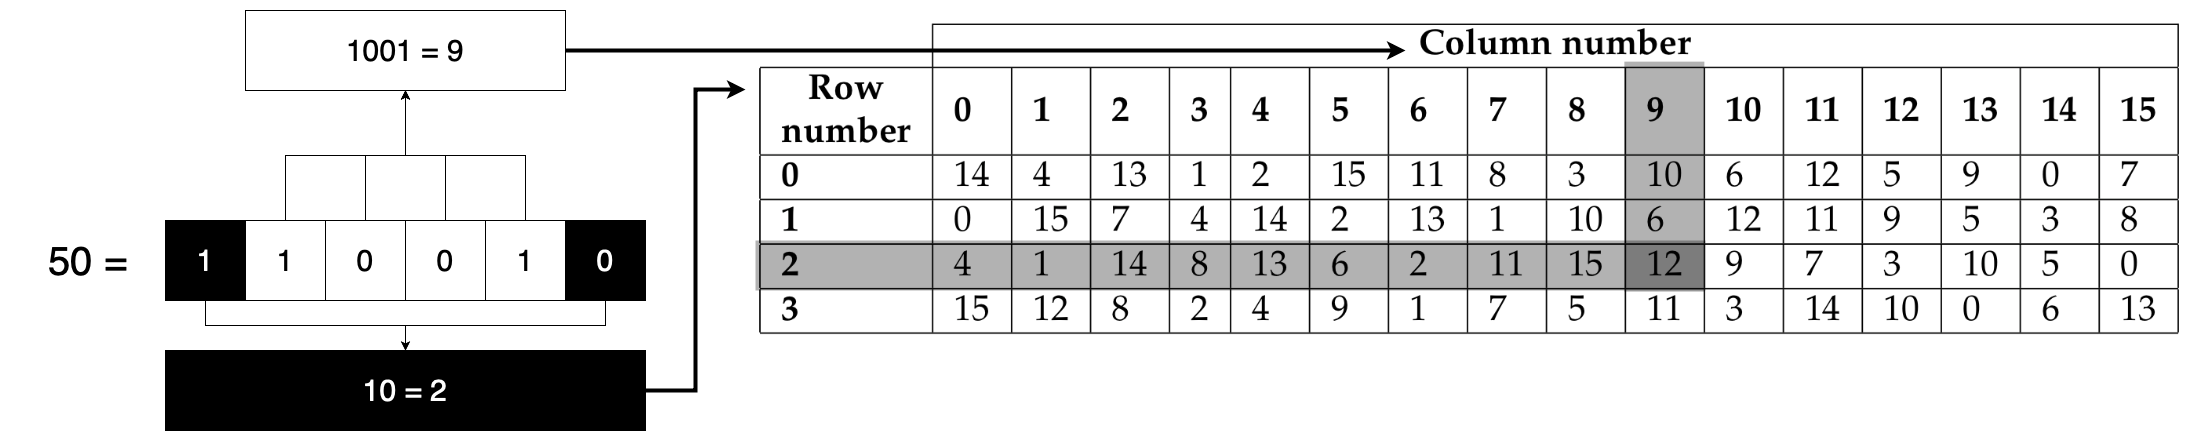
\includegraphics[scale=0.2]{des-sbox-indexing.png}
    \caption{Usage of the $S_1$ DES $S$-Box}
    \label{fig:des-indexing}
\end{figure}

An output integer is denoted by $y = (y_1, y_2, y_3, y_4)$, also  considering the binary representation of the integer from left to right. For $x = 50$, the $S_1$ output is $12$, thus $y_1 = 1, y_2 = 1, y_3 = 0$ and $y_4 = 0$, since the binary representation of 12 is $1100$. In vectorial Boolean function notation, $S_1(1, 1, 0, 0, 1, 0) = (1, 1, 0, 0)$.

Applying the method of Section \ref{sec:finding-anf}, we obtain the ANFs for each output bit $y_i$, $1 \leq i \leq 4$ of $S_1$, and they directly show the relationship with the each input bit $x_j$, $1 \leq j \leq 6$, allowing us to assess the diffusion property.

Equations \ref{eq:s1y1}, \ref{eq:s1y2}, \ref{eq:s1y3} and \ref{eq:s1y4} are the obtained Algebraic Normal Forms of $y_1, y_2, y_3$ and $y_4$, respectively, regarding the $S$-Box $S_1$ (see Table \ref{tab:DES_S-Box_1}) of DES.

\begin{dmath}\label{eq:s1y1}
    y_1 = 1+x_6+x_5+x_4x_5x_6+x_3+x_3x_4+x_3x_4x_6+x_3x_4x_5+x_2+x_2x_3+x_2x_3x_4+x_1+x_1x_5+x_1x_4+x_1x_4x_6+x_1x_3x_5+x_1x_3x_4+x_1x_3x_4x_6+x_1x_3x_4x_5+x_1x_2x_5x_6+x_1x_2x_4+x_1x_2x_4x_6+x_1x_2x_4x_5+x_1x_2x_3+x_1x_2x_3x_5x_6+x_1x_2x_3x_4+x_1x_2x_3x_4x_6,
\end{dmath}

\begin{dmath}\label{eq:s1y2}
    y_2 = 1+x_6+x_5x_6+x_4x_6+x_4x_5+x_3+x_3x_5+x_3x_5x_6+x_3x_4x_6+x_3x_4x_5x_6+x_2+x_2x_6+x_2x_4+x_2x_4x_6+x_2x_4x_5+x_2x_3x_6+x_1x_6+x_1x_5+x_1x_4x_5+x_1x_3+x_1x_3x_5x_6+x_1x_3x_4+x_1x_3x_4x_5x_6+x_1x_2+x_1x_2x_6+x_1x_2x_5+x_1x_2x_4x_5x_6+x_1x_2x_3+x_1x_2x_3x_6+x_1x_2x_3x_5+x_1x_2x_3x_5x_6+x_1x_2x_3x_4+x_1x_2x_3x_4x_6,
\end{dmath}

\begin{dmath}\label{eq:s1y3}
    y_3 = 1+x_6+x_5+x_4+x_4x_5+x_4x_5x_6+x_3x_6+x_3x_5+x_3x_4+x_3x_4x_6+x_2x_6+x_2x_5+x_2x_4+x_2x_4x_6+x_2x_4x_5x_6+x_2x_3+x_2x_3x_6+x_2x_3x_5+x_2x_3x_4+x_2x_3x_4x_6+x_1+x_1x_5+x_1x_5x_6+x_1x_3x_4+x_1x_3x_4x_5x_6+x_1x_2+x_1x_2x_6+x_1x_2x_5x_6+x_1x_2x_4+x_1x_2x_4x_6+x_1x_2x_4x_5+x_1x_2x_4x_5x_6+x_1x_2x_3+x_1x_2x_3x_6+x_1x_2x_3x_5+x_1x_2x_3x_5x_6+x_1x_2x_3x_4+x_1x_2x_3x_4x_6,
\end{dmath}

\begin{dmath}\label{eq:s1y4}
    y_4 = x_5x_6+x_4+x_3x_5+x_2+x_2x_6+x_2x_5+x_2x_4x_6+x_2x_4x_5+x_2x_3x_6+x_2x_3x_5x_6+x_1x_6+x_1x_5+x_1x_5x_6+x_1x_4+x_1x_4x_6+x_1x_4x_5+x_1x_3+x_1x_3x_5+x_1x_3x_4+x_1x_3x_4x_6+x_1x_3x_4x_5+x_1x_3x_4x_5x_6+x_1x_2x_5+x_1x_2x_5x_6+x_1x_2x_4x_5+x_1x_2x_3+x_1x_2x_3x_5x_6+x_1x_2x_3x_4+x_1x_2x_3x_4x_6.
\end{dmath}

For convenience, the concept of diffusion is presented here again.

\begin{concept}[Diffusion]
Refers to the influence of each plaintext (key) bit upon the ciphertext bits. This influence must be as widespread as possible.
\end{concept}

Although it refers to plaintext and ciphertext bits, for the moment, we restrict the analysis to the $S$-boxes --- we evaluate the influence of each input bit upon the output bits. For $S_1$, we see clearly that $y_1$ depends on $x_1, x_2, x_3, x_4, x_5$ and $x_6$, since they are present in the ANF. The same holds for $y_2, y_3$ and $y_4$, thus $y_2$ depends on all input bits, and so do $y_3$ and $y_4$. Each input bit spreads its influence to all output bits. Therefore, $S_1$ \emph{achieves complete diffusion}.

Table \ref{tab:DES_S-Box_2} shows $S_2$, and Equations \ref{eq:s2y1} to \ref{eq:s2y4} show the respective ANFs.

\begin{table}[h!]
\centering
\begin{tabular}{l|l|l|l|l|l|l|l|l|l|l|l|l|l|l|l|l|}
\cline{2-17}
                                                                                    & \multicolumn{16}{c|}{\textbf{Column number $(x_2, x_3, x_4, x_5)$}}                                                                                                                                                                        \\ \hline
\multicolumn{1}{|c|}{\textbf{\begin{tabular}[c]{@{}c@{}}Row\\ number $(x_1, x_6)$\end{tabular}}} & \textbf{0} & \textbf{1} & \textbf{2} & \textbf{3} & \textbf{4} & \textbf{5} & \textbf{6} & \textbf{7} & \textbf{8} & \textbf{9} & \textbf{10} & \textbf{11} & \textbf{12} & \textbf{13} & \textbf{14} & \textbf{15} \\ \hline
\multicolumn{1}{|l|}{\textbf{0}}                                                    & 15         & 1          & 8          & 14         & 6          & 11         & 3          & 4          & 9          & 7          & 2           & 13          & 12          & 0           & 5           & 10          \\ \hline
\multicolumn{1}{|l|}{\textbf{1}}                                                    & 3          & 13         & 4          & 7          & 15         & 2          & 8          & 14         & 12         & 0          & 1           & 10          & 6           & 9           & 11          & 5           \\ \hline
\multicolumn{1}{|l|}{\textbf{2}}                                                    & 0          & 14         & 7          & 11         & 10         & 4          & 13         & 1          & 5          & 8          & 12          & 6           & 9           & 3           & 2           & 15          \\ \hline
\multicolumn{1}{|l|}{\textbf{3}}                                                    & 13         & 8          & 10         & 1          & 3          & 15         & 4          & 2          & 11         & 6          & 7           & 12          & 0           & 5           & 14          & 9           \\ \hline
\end{tabular}
\caption{DES S-Box $S_2$}
\label{tab:DES_S-Box_2}
\end{table}

\begin{dmath}\label{eq:s2y1}
    y_1 = 1+x_6+x_5+x_4x_5+x_3+x_2x_6+x_2x_4+x_2x_4x_5+x_2x_3+x_2x_3x_6+x_1+x_1x_5x_6+x_1x_4x_5+x_1x_4x_5x_6+x_1x_3x_5x_6+x_1x_2x_6+x_1x_2x_5x_6+x_1x_2x_4x_5+x_1x_2x_4x_5x_6+x_1x_2x_3+x_1x_2x_3x_6,
\end{dmath}

\begin{dmath}\label{eq:s2y2}
    y_2 = 1+x_6+x_5+x_4+x_4x_5x_6+x_3x_6+x_3x_4x_5x_6+x_2+x_2x_4+x_2x_4x_6+x_2x_3+x_1+x_1x_2x_4x_5+x_1x_2x_4x_5x_6+x_1x_2x_3x_5+x_1x_2x_3x_5x_6,
\end{dmath}

\begin{dmath}\label{eq:s2y3}
    y_3 = 1+x_5+x_4+x_3x_5+x_3x_4+x_3x_4x_6+x_3x_4x_5+x_2+x_2x_5x_6+x_2x_4x_6+x_2x_4x_5x_6+x_2x_3x_6+x_1+x_1x_5x_6+x_1x_4x_5+x_1x_3+x_1x_3x_5+x_1x_3x_4+x_1x_3x_4x_6+x_1x_3x_4x_5+x_1x_2+x_1x_2x_6+x_1x_2x_5+x_1x_2x_4+x_1x_2x_4x_6+x_1x_2x_4x_5x_6+x_1x_2x_3+x_1x_2x_3x_5+x_1x_2x_3x_5x_6+x_1x_2x_3x_4,
\end{dmath}

\begin{dmath}\label{eq:s2y4}
    y_4 = 1+x_4+x_4x_5x_6+x_3+x_3x_6+x_3x_5+x_2x_6+x_2x_4x_5+x_2x_4x_5x_6+x_2x_3x_5+x_2x_3x_5x_6+x_1+x_1x_6+x_1x_5x_6+x_1x_4x_5x_6+x_1x_3+x_1x_3x_6+x_1x_3x_5+x_1x_3x_5x_6+x_1x_2+x_1x_2x_5+x_1x_2x_5x_6+x_1x_2x_4x_6+x_1x_2x_3x_6+x_1x_2x_3x_5x_6.
\end{dmath}

Table \ref{tab:DES_S-Box_3} shows $S_3$, and Equations \ref{eq:s3y1} to \ref{eq:s3y4} show the respective ANFs.

\begin{table}[h!]
\centering
\begin{tabular}{l|l|l|l|l|l|l|l|l|l|l|l|l|l|l|l|l|}
\cline{2-17}
                                                                                    & \multicolumn{16}{c|}{\textbf{Column number $(x_2, x_3, x_4, x_5)$}}                                                                                                                                                                        \\ \hline
\multicolumn{1}{|c|}{\textbf{\begin{tabular}[c]{@{}c@{}}Row\\ number $(x_1, x_6)$\end{tabular}}} & \textbf{0} & \textbf{1} & \textbf{2} & \textbf{3} & \textbf{4} & \textbf{5} & \textbf{6} & \textbf{7} & \textbf{8} & \textbf{9} & \textbf{10} & \textbf{11} & \textbf{12} & \textbf{13} & \textbf{14} & \textbf{15} \\ \hline
\multicolumn{1}{|l|}{\textbf{0}}                                                    & 10         & 0          & 9          & 14         & 6          & 3          & 15         & 5          & 1          & 13         & 12          & 7           & 11          & 4           & 2           & 8           \\ \hline
\multicolumn{1}{|l|}{\textbf{1}}                                                    & 13         & 7          & 0          & 9          & 3          & 4          & 6          & 10         & 2          & 8          & 5           & 14          & 12          & 11          & 15          & 1           \\ \hline
\multicolumn{1}{|l|}{\textbf{2}}                                                    & 13         & 6          & 4          & 9          & 8          & 15         & 3          & 0          & 11         & 1          & 2           & 12          & 5           & 10          & 14          & 7           \\ \hline
\multicolumn{1}{|l|}{\textbf{3}}                                                    & 1          & 10         & 13         & 0          & 6          & 9          & 8          & 7          & 4          & 15         & 14          & 3           & 11          & 5           & 2           & 12          \\ \hline
\end{tabular}
\caption{DES S-Box $S_3$}
\label{tab:DES_S-Box_3}
\end{table}

\begin{dmath}\label{eq:s3y1}
    y_1 = 1+x_6+x_5+x_4x_5+x_3+x_2x_6+x_2x_4+x_2x_4x_5+x_2x_3+x_2x_3x_6+x_1+x_1x_5x_6+x_1x_4x_5+x_1x_4x_5x_6+x_1x_3x_5x_6+x_1x_2x_6+x_1x_2x_5x_6+x_1x_2x_4x_5+x_1x_2x_4x_5x_6+x_1x_2x_3+x_1x_2x_3x_6,
\end{dmath}

\begin{dmath}\label{eq:s3y2}
    y_2 = 1+x_6+x_5+x_4+x_4x_5x_6+x_3x_6+x_3x_4x_5x_6+x_2+x_2x_4+x_2x_4x_6+x_2x_3+x_1+x_1x_2x_4x_5+x_1x_2x_4x_5x_6+x_1x_2x_3x_5+x_1x_2x_3x_5x_6,
\end{dmath}

\begin{dmath}\label{eq:s3y3}
    y_3 = 1+x_5+x_4+x_3x_5+x_3x_4+x_3x_4x_6+x_3x_4x_5+x_2+x_2x_5x_6+x_2x_4x_6+x_2x_4x_5x_6+x_2x_3x_6+x_1+x_1x_5x_6+x_1x_4x_5+x_1x_3+x_1x_3x_5+x_1x_3x_4+x_1x_3x_4x_6+x_1x_3x_4x_5+x_1x_2+x_1x_2x_6+x_1x_2x_5+x_1x_2x_4+x_1x_2x_4x_6+x_1x_2x_4x_5x_6+x_1x_2x_3+x_1x_2x_3x_5+x_1x_2x_3x_5x_6+x_1x_2x_3x_4,
\end{dmath}

\begin{dmath}\label{eq:s3y4}
    y_4 = 1+x_4+x_4x_5x_6+x_3+x_3x_6+x_3x_5+x_2x_6+x_2x_4x_5+x_2x_4x_5x_6+x_2x_3x_5+x_2x_3x_5x_6+x_1+x_1x_6+x_1x_5x_6+x_1x_4x_5x_6+x_1x_3+x_1x_3x_6+x_1x_3x_5+x_1x_3x_5x_6+x_1x_2+x_1x_2x_5+x_1x_2x_5x_6+x_1x_2x_4x_6+x_1x_2x_3x_6+x_1x_2x_3x_5x_6.
\end{dmath}

Table \ref{tab:DES_S-Box_4} shows $S_4$, and Equations \ref{eq:s4y1} to \ref{eq:s4y4} show the respective ANFs.

\begin{table}[h!]
\centering
\begin{tabular}{l|l|l|l|l|l|l|l|l|l|l|l|l|l|l|l|l|}
\cline{2-17}
                                                                                    & \multicolumn{16}{c|}{\textbf{Column number $(x_2, x_3, x_4, x_5)$}}                                                                                                                                                                        \\ \hline
\multicolumn{1}{|c|}{\textbf{\begin{tabular}[c]{@{}c@{}}Row\\ number $(x_1, x_6)$\end{tabular}}} & \textbf{0} & \textbf{1} & \textbf{2} & \textbf{3} & \textbf{4} & \textbf{5} & \textbf{6} & \textbf{7} & \textbf{8} & \textbf{9} & \textbf{10} & \textbf{11} & \textbf{12} & \textbf{13} & \textbf{14} & \textbf{15} \\ \hline
\multicolumn{1}{|l|}{\textbf{0}}                                                    & 7          & 13         & 14         & 3          & 0          & 6          & 9          & 10         & 1          & 2          & 8           & 5           & 11          & 12          & 4           & 15          \\ \hline
\multicolumn{1}{|l|}{\textbf{1}}                                                    & 13         & 8          & 11         & 5          & 6          & 15         & 0          & 3          & 4          & 7          & 2           & 12          & 1           & 10          & 14          & 9           \\ \hline
\multicolumn{1}{|l|}{\textbf{2}}                                                    & 10         & 6          & 9          & 0          & 12         & 11         & 7          & 13         & 15         & 1          & 3           & 14          & 5           & 2           & 8           & 4           \\ \hline
\multicolumn{1}{|l|}{\textbf{3}}                                                    & 3          & 15         & 0          & 6          & 10         & 1          & 13         & 8          & 9          & 4          & 5           & 11          & 12          & 7           & 2           & 14          \\ \hline
\end{tabular}
\caption{DES S-Box $S_4$}
\label{tab:DES_S-Box_4}
\end{table}

\begin{dmath}\label{eq:s4y1}
    y_1 = x_6+x_5+x_5x_6+x_4+x_4x_6+x_4x_5x_6+x_3x_6+x_3x_5+x_2x_6+x_2x_5+x_2x_5x_6+x_2x_4x_5+x_2x_4x_5x_6+x_2x_3+x_2x_3x_5+x_2x_3x_5x_6+x_2x_3x_4x_6+x_1+x_1x_5x_6+x_1x_4+x_1x_4x_6+x_1x_3x_5x_6+x_1x_3x_4+x_1x_3x_4x_6+x_1x_3x_4x_5+x_1x_3x_4x_5x_6+x_1x_2x_5+x_1x_2x_5x_6+x_1x_2x_4+x_1x_2x_4x_5+x_1x_2x_3x_5+x_1x_2x_3x_5x_6+x_1x_2x_3x_4,
\end{dmath}

\begin{dmath}\label{eq:s4y2}
    y_2 = 1+x_5x_6+x_4x_6+x_4x_5+x_4x_5x_6+x_3+x_3x_6+x_3x_5+x_2+x_2x_6+x_2x_5x_6+x_2x_4x_5x_6+x_2x_3+x_2x_3x_5x_6+x_2x_3x_4+x_2x_3x_4x_6+x_1+x_1x_5+x_1x_5x_6+x_1x_4x_6+x_1x_3x_5+x_1x_3x_5x_6+x_1x_3x_4x_6+x_1x_3x_4x_5x_6+x_1x_2x_5x_6+x_1x_2x_4+x_1x_2x_4x_5+x_1x_2x_3x_5x_6+x_1x_2x_3x_4,
\end{dmath}

\begin{dmath}\label{eq:s4y3}
    y_3 = 1+x_6+x_5+x_5x_6+x_4x_6+x_4x_5+x_3+x_3x_4x_5+x_3x_4x_5x_6+x_2+x_2x_6+x_2x_5x_6+x_2x_4x_5x_6+x_2x_3x_6+x_2x_3x_4+x_2x_3x_4x_6+x_1x_6+x_1x_5+x_1x_5x_6+x_1x_4+x_1x_4x_6+x_1x_4x_5+x_1x_4x_5x_6+x_1x_3x_6+x_1x_3x_5+x_1x_3x_4x_5+x_1x_3x_4x_5x_6+x_1x_2+x_1x_2x_5+x_1x_2x_4+x_1x_2x_4x_5+x_1x_2x_3x_6+x_1x_2x_3x_5+x_1x_2x_3x_5x_6+x_1x_2x_3x_4,
\end{dmath}

\begin{dmath}\label{eq:s4y4}
    y_4 = 1+x_5x_6+x_4+x_4x_6+x_4x_5+x_3+x_3x_4x_5x_6+x_2x_6+x_2x_5+x_2x_5x_6+x_2x_4x_5+x_2x_4x_5x_6+x_2x_3+x_2x_3x_6+x_2x_3x_4x_6+x_1+x_1x_6+x_1x_5x_6+x_1x_4x_6+x_1x_4x_5x_6+x_1x_3+x_1x_3x_6+x_1x_3x_5+x_1x_3x_4x_5x_6+x_1x_2+x_1x_2x_5+x_1x_2x_4+x_1x_2x_4x_5+x_1x_2x_3+x_1x_2x_3x_6+x_1x_2x_3x_5x_6+x_1x_2x_3x_4.
\end{dmath}

Table \ref{tab:DES_S-Box_5} shows $S_5$, and Equations \ref{eq:s5y1} to \ref{eq:s5y4} show the respective ANFs.

\begin{table}[h!]
\centering
\begin{tabular}{l|l|l|l|l|l|l|l|l|l|l|l|l|l|l|l|l|}
\cline{2-17}
                                                                                    & \multicolumn{16}{c|}{\textbf{Column number $(x_2, x_3, x_4, x_5)$}}                                                                                                                                                                        \\ \hline
\multicolumn{1}{|c|}{\textbf{\begin{tabular}[c]{@{}c@{}}Row\\ number $(x_1, x_6)$\end{tabular}}} & \textbf{0} & \textbf{1} & \textbf{2} & \textbf{3} & \textbf{4} & \textbf{5} & \textbf{6} & \textbf{7} & \textbf{8} & \textbf{9} & \textbf{10} & \textbf{11} & \textbf{12} & \textbf{13} & \textbf{14} & \textbf{15} \\ \hline
\multicolumn{1}{|l|}{\textbf{0}}                                                    & 2          & 12         & 4          & 1          & 7          & 10         & 11         & 6          & 8          & 5          & 3           & 15          & 13          & 0           & 14          & 9           \\ \hline
\multicolumn{1}{|l|}{\textbf{1}}                                                    & 14         & 11         & 2          & 12         & 4          & 7          & 13         & 1          & 5          & 0          & 15          & 10          & 3           & 9           & 8           & 6           \\ \hline
\multicolumn{1}{|l|}{\textbf{2}}                                                    & 4          & 2          & 1          & 11         & 10         & 13         & 7          & 8          & 15         & 9          & 12          & 5           & 6           & 3           & 0           & 14          \\ \hline
\multicolumn{1}{|l|}{\textbf{3}}                                                    & 11         & 8          & 12         & 7          & 1          & 14         & 2          & 13         & 6          & 15         & 0           & 9           & 10          & 4           & 5           & 3           \\ \hline
\end{tabular}
\caption{DES S-Box $S_5$}
\label{tab:DES_S-Box_5}
\end{table}

\begin{dmath}\label{eq:s5y1}
    y_1 = x_6+x_5+x_5x_6+x_4x_6+x_4x_5+x_3x_6+x_3x_4+x_3x_4x_6+x_3x_4x_5+x_3x_4x_5x_6+x_2+x_2x_4+x_2x_4x_6+x_2x_4x_5+x_2x_3x_6+x_2x_3x_5x_6+x_1x_5+x_1x_5x_6+x_1x_4x_6+x_1x_3+x_1x_3x_6+x_1x_3x_5x_6+x_1x_3x_4x_5+x_1x_2x_5x_6+x_1x_2x_4+x_1x_2x_4x_6+x_1x_2x_4x_5+x_1x_2x_4x_5x_6+x_1x_2x_3x_6+x_1x_2x_3x_4,
\end{dmath}

\begin{dmath}\label{eq:s5y2}
    y_2 = x_6+x_5+x_4+x_3+x_3x_6+x_3x_5x_6+x_3x_4x_6+x_3x_4x_5x_6+x_2x_4+x_2x_3x_6+x_2x_3x_4x_6+x_1+x_1x_5x_6+x_1x_4x_5+x_1x_4x_5x_6+x_1x_3x_4x_5+x_1x_2x_6+x_1x_2x_4x_6+x_1x_2x_3+x_1x_2x_3x_6+x_1x_2x_3x_4+x_1x_2x_3x_4x_6,
\end{dmath}

\begin{dmath}\label{eq:s5y3}
    y_3 = 1+x_5+x_5x_6+x_4+x_4x_6+x_4x_5+x_3x_6+x_3x_5+x_3x_4+x_3x_4x_6+x_3x_4x_5+x_3x_4x_5x_6+x_2+x_2x_5+x_2x_5x_6+x_2x_4x_6+x_2x_4x_5+x_2x_3x_5+x_2x_3x_5x_6+x_2x_3x_4+x_2x_3x_4x_6+x_1+x_1x_6+x_1x_5x_6+x_1x_4+x_1x_4x_5+x_1x_3+x_1x_3x_6+x_1x_3x_5+x_1x_3x_4+x_1x_3x_4x_6+x_1x_3x_4x_5+x_1x_3x_4x_5x_6+x_1x_2x_6+x_1x_2x_5+x_1x_2x_4+x_1x_2x_4x_5x_6+x_1x_2x_3+x_1x_2x_3x_5x_6+x_1x_2x_3x_4+x_1x_2x_3x_4x_6,
\end{dmath}

\begin{dmath}\label{eq:s5y4}
    y_4 = x_5x_6+x_4x_5+x_3+x_3x_6+x_3x_5+x_3x_5x_6+x_3x_4x_6+x_3x_4x_5+x_3x_4x_5x_6+x_2x_6+x_2x_5+x_2x_5x_6+x_2x_4+x_2x_4x_6+x_2x_4x_5x_6+x_2x_3x_5+x_1x_6+x_1x_4+x_1x_4x_5+x_1x_3+x_1x_3x_6+x_1x_3x_4x_6+x_1x_3x_4x_5+x_1x_3x_4x_5x_6+x_1x_2+x_1x_2x_6+x_1x_2x_5+x_1x_2x_5x_6+x_1x_2x_4+x_1x_2x_4x_5+x_1x_2x_3+x_1x_2x_3x_6+x_1x_2x_3x_5+x_1x_2x_3x_5x_6+x_1x_2x_3x_4.
\end{dmath}

Table \ref{tab:DES_S-Box_6} shows $S_6$, and Equations \ref{eq:s6y1} to \ref{eq:s6y4} show the respective ANFs.

\begin{table}[h!]
\centering
\begin{tabular}{l|l|l|l|l|l|l|l|l|l|l|l|l|l|l|l|l|}
\cline{2-17}
                                                                                    & \multicolumn{16}{c|}{\textbf{Column number $(x_2, x_3, x_4, x_5)$}}                                                                                                                                                                        \\ \hline
\multicolumn{1}{|c|}{\textbf{\begin{tabular}[c]{@{}c@{}}Row\\ number $(x_1, x_6)$\end{tabular}}} & \textbf{0} & \textbf{1} & \textbf{2} & \textbf{3} & \textbf{4} & \textbf{5} & \textbf{6} & \textbf{7} & \textbf{8} & \textbf{9} & \textbf{10} & \textbf{11} & \textbf{12} & \textbf{13} & \textbf{14} & \textbf{15} \\ \hline
\multicolumn{1}{|l|}{\textbf{0}}                                                    & 12         & 1          & 10         & 15         & 9          & 2          & 6          & 8          & 0          & 13         & 3           & 4           & 14          & 7           & 5           & 11          \\ \hline
\multicolumn{1}{|l|}{\textbf{1}}                                                    & 10         & 15         & 4          & 2          & 7          & 12         & 9          & 5          & 6          & 1          & 13          & 14          & 0           & 11          & 3           & 8           \\ \hline
\multicolumn{1}{|l|}{\textbf{2}}                                                    & 9          & 14         & 15         & 5          & 2          & 8          & 12         & 3          & 7          & 0          & 4           & 10          & 1           & 13          & 11          & 6           \\ \hline
\multicolumn{1}{|l|}{\textbf{3}}                                                    & 4          & 3          & 2          & 12         & 9          & 5          & 15         & 10         & 11         & 14         & 1           & 7           & 6           & 0           & 8           & 13          \\ \hline
\end{tabular}
\caption{DES S-Box $S_6$}
\label{tab:DES_S-Box_6}
\end{table}

\begin{dmath}\label{eq:s6y1}
    y_1 = 1+x_5+x_5x_6+x_4x_6+x_4x_5+x_4x_5x_6+x_3x_6+x_3x_5x_6+x_3x_4+x_3x_4x_6+x_3x_4x_5+x_3x_4x_5x_6+x_2+x_2x_3+x_2x_3x_4x_6+x_1x_6+x_1x_5+x_1x_5x_6+x_1x_4x_6+x_1x_4x_5x_6+x_1x_3+x_1x_3x_6+x_1x_3x_5+x_1x_3x_5x_6+x_1x_2x_4x_6+x_1x_2x_4x_5x_6+x_1x_2x_3x_6+x_1x_2x_3x_5x_6+x_1x_2x_3x_4x_6,
\end{dmath}

\begin{dmath}\label{eq:s6y2}
    y_2 = 1+x_6+x_5+x_4+x_3+x_3x_5+x_3x_4x_5+x_2+x_2x_4+x_2x_4x_5x_6+x_1+x_1x_4x_5+x_1x_4x_5x_6+x_1x_3+x_1x_3x_6+x_1x_3x_5x_6+x_1x_3x_4x_5+x_1x_2x_4x_5+x_1x_2x_3+x_1x_2x_3x_6+x_1x_2x_3x_5+x_1x_2x_3x_5x_6+x_1x_2x_3x_4x_6,
\end{dmath}

\begin{dmath}\label{eq:s6y3}
    y_3 = x_6+x_4+x_4x_5x_6+x_3x_5+x_2x_5x_6+x_2x_4x_5+x_2x_3+x_2x_3x_5+x_1x_6+x_1x_5+x_1x_4x_5x_6+x_1x_3+x_1x_3x_6+x_1x_3x_5+x_1x_3x_5x_6+x_1x_2+x_1x_2x_4x_5+x_1x_2x_4x_5x_6+x_1x_2x_3+x_1x_2x_3x_5x_6,
\end{dmath}

\begin{dmath}\label{eq:s6y4}
    y_4 = x_5+x_4x_5x_6+x_3+x_3x_4+x_3x_4x_6+x_3x_4x_5+x_3x_4x_5x_6+x_2x_4+x_2x_4x_5x_6+x_2x_3+x_2x_3x_4+x_2x_3x_4x_6+x_1+x_1x_6+x_1x_4x_5+x_1x_4x_5x_6+x_1x_3x_5+x_1x_3x_4+x_1x_3x_4x_6+x_1x_3x_4x_5+x_1x_3x_4x_5x_6+x_1x_2x_6+x_1x_2x_4x_6+x_1x_2x_4x_5x_6+x_1x_2x_3x_6.
\end{dmath}

Table \ref{tab:DES_S-Box_7} shows $S_7$, and Equations \ref{eq:s7y1} to \ref{eq:s7y4} show the respective ANFs.

\begin{table}[h!]
\centering
\begin{tabular}{l|l|l|l|l|l|l|l|l|l|l|l|l|l|l|l|l|}
\cline{2-17}
                                                                                    & \multicolumn{16}{c|}{\textbf{Column number $(x_2, x_3, x_4, x_5)$}}                                                                                                                                                                        \\ \hline
\multicolumn{1}{|c|}{\textbf{\begin{tabular}[c]{@{}c@{}}Row\\ number $(x_1, x_6)$\end{tabular}}} & \textbf{0} & \textbf{1} & \textbf{2} & \textbf{3} & \textbf{4} & \textbf{5} & \textbf{6} & \textbf{7} & \textbf{8} & \textbf{9} & \textbf{10} & \textbf{11} & \textbf{12} & \textbf{13} & \textbf{14} & \textbf{15} \\ \hline
\multicolumn{1}{|l|}{\textbf{0}}                                                    & 4          & 11         & 2          & 14         & 15         & 0          & 8          & 13         & 3          & 12         & 9           & 7           & 5           & 10          & 6           & 1           \\ \hline
\multicolumn{1}{|l|}{\textbf{1}}                                                    & 13         & 0          & 11         & 7          & 4          & 9          & 1          & 10         & 14         & 3          & 5           & 12          & 2           & 15          & 8           & 6           \\ \hline
\multicolumn{1}{|l|}{\textbf{2}}                                                    & 1          & 4          & 11         & 13         & 12         & 3          & 7          & 14         & 10         & 15         & 6           & 8           & 0           & 5           & 9           & 2           \\ \hline
\multicolumn{1}{|l|}{\textbf{3}}                                                    & 6          & 11         & 13         & 8          & 1          & 4          & 10         & 7          & 9          & 5          & 0           & 15          & 14          & 2           & 3           & 12          \\ \hline
\end{tabular}
\caption{DES S-Box $S_7$}
\label{tab:DES_S-Box_7}
\end{table}

\begin{dmath}\label{eq:s7y1}
    y_1 = x_6+x_5+x_3+x_3x_4x_5+x_3x_4x_5x_6+x_2x_4+x_2x_3+x_2x_3x_6+x_2x_3x_4+x_2x_3x_4x_6+x_1x_6+x_1x_5+x_1x_5x_6+x_1x_4+x_1x_4x_5x_6+x_1x_3x_6+x_1x_3x_5+x_1x_3x_4x_5+x_1x_3x_4x_5x_6+x_1x_2+x_1x_2x_4+x_1x_2x_4x_5+x_1x_2x_3+x_1x_2x_3x_6+x_1x_2x_3x_5+x_1x_2x_3x_4+x_1x_2x_3x_4x_6,
\end{dmath}

\begin{dmath}\label{eq:s7y2}
    y_2 = 1+x_5+x_4+x_3x_4x_5x_6+x_2+x_2x_6+x_2x_4+x_2x_4x_5x_6+x_2x_3+x_1+x_1x_6+x_1x_4+x_1x_3+x_1x_3x_4x_5+x_1x_2+x_1x_2x_4x_6+x_1x_2x_4x_5x_6+x_1x_2x_3x_6+x_1x_2x_3x_4,
\end{dmath}

\begin{dmath}\label{eq:s7y3}
    y_3 = x_5+x_5x_6+x_4+x_4x_5+x_4x_5x_6+x_3+x_3x_6+x_3x_4x_6+x_3x_4x_5x_6+x_2+x_2x_4x_5+x_2x_4x_5x_6+x_2x_3x_4x_6+x_1x_6+x_1x_5+x_1x_5x_6+x_1x_3+x_1x_3x_5+x_1x_3x_5x_6+x_1x_3x_4x_6+x_1x_3x_4x_5x_6+x_1x_2x_4+x_1x_2x_4x_5+x_1x_2x_3+x_1x_2x_3x_6+x_1x_2x_3x_5+x_1x_2x_3x_5x_6+x_1x_2x_3x_4x_6,
\end{dmath}

\begin{dmath}\label{eq:s7y4}
    y_4 = x_6+x_5+x_4x_5+x_3+x_3x_4+x_3x_4x_5+x_2+x_2x_4x_6+x_2x_4x_5x_6+x_2x_3+x_1+x_1x_4x_6+x_1x_4x_5x_6+x_1x_3x_4x_6+x_1x_3x_4x_5x_6+x_1x_2x_5x_6+x_1x_2x_4x_6+x_1x_2x_3x_6.
\end{dmath}

Table \ref{tab:DES_S-Box_8} shows $S_8$, and Equations \ref{eq:s8y1} to \ref{eq:s8y4} show the respective ANFs.

\begin{table}[h!]
\centering
\begin{tabular}{l|l|l|l|l|l|l|l|l|l|l|l|l|l|l|l|l|}
\cline{2-17}
                                                                                    & \multicolumn{16}{c|}{\textbf{Column number $(x_2, x_3, x_4, x_5)$}}                                                                                                                                                                        \\ \hline
\multicolumn{1}{|c|}{\textbf{\begin{tabular}[c]{@{}c@{}}Row\\ number $(x_1, x_6)$\end{tabular}}} & \textbf{0} & \textbf{1} & \textbf{2} & \textbf{3} & \textbf{4} & \textbf{5} & \textbf{6} & \textbf{7} & \textbf{8} & \textbf{9} & \textbf{10} & \textbf{11} & \textbf{12} & \textbf{13} & \textbf{14} & \textbf{15} \\ \hline
\multicolumn{1}{|l|}{\textbf{0}}                                                    & 13         & 2          & 8          & 4          & 6          & 15         & 11         & 1          & 10         & 9          & 3           & 14          & 5           & 0           & 12          & 7           \\ \hline
\multicolumn{1}{|l|}{\textbf{1}}                                                    & 1          & 15         & 13         & 8          & 10         & 3          & 7          & 4          & 12         & 5          & 6           & 11          & 0           & 14          & 9           & 2           \\ \hline
\multicolumn{1}{|l|}{\textbf{2}}                                                    & 7          & 11         & 4          & 1          & 9          & 12         & 14         & 2          & 0          & 6          & 10          & 13          & 15          & 3           & 5           & 8           \\ \hline
\multicolumn{1}{|l|}{\textbf{3}}                                                    & 2          & 1          & 14         & 7          & 4          & 10         & 8          & 13         & 15         & 12         & 9           & 0           & 3           & 5           & 6           & 11          \\ \hline
\end{tabular}
\caption{DES S-Box $S_8$}
\label{tab:DES_S-Box_8}
\end{table}

\begin{dmath}\label{eq:s8y1}
    y_1 = 1+x_6+x_5+x_4x_6+x_4x_5x_6+x_3+x_3x_4+x_3x_4x_6+x_2x_6+x_2x_5+x_2x_5x_6+x_2x_4+x_2x_4x_6+x_2x_4x_5+x_2x_3x_4+x_2x_3x_4x_6+x_1+x_1x_6+x_1x_5x_6+x_1x_4x_5+x_1x_4x_5x_6+x_1x_3x_6+x_1x_3x_5+x_1x_3x_4+x_1x_3x_4x_6+x_1x_2x_4x_6+x_1x_2x_4x_5x_6+x_1x_2x_3x_6+x_1x_2x_3x_5x_6+x_1x_2x_3x_4+x_1x_2x_3x_4x_6,
\end{dmath}

\begin{dmath}\label{eq:s8y2}
    y_2 = 1+x_6+x_5+x_4+x_3x_5+x_2+x_2x_5+x_2x_4+x_2x_4x_5+x_2x_3+x_1x_5x_6+x_1x_4+x_1x_4x_6+x_1x_3+x_1x_3x_5+x_1x_3x_5x_6+x_1x_3x_4+x_1x_3x_4x_6+x_1x_2x_5+x_1x_2x_4+x_1x_2x_4x_5+x_1x_2x_3+x_1x_2x_3x_4+x_1x_2x_3x_4x_6,
\end{dmath}

\begin{dmath}\label{eq:s8y3}
    y_3 = x_5+x_4x_5+x_3+x_3x_5+x_2+x_2x_6+x_2x_5x_6+x_2x_4x_6+x_2x_4x_5x_6+x_2x_3x_6+x_2x_3x_4x_6+x_1+x_1x_5+x_1x_5x_6+x_1x_4+x_1x_4x_6+x_1x_4x_5+x_1x_4x_5x_6+x_1x_3x_5+x_1x_2x_5+x_1x_2x_4x_5x_6+x_1x_2x_3x_5+x_1x_2x_3x_5x_6,
\end{dmath}

\begin{dmath}\label{eq:s8y4}
    y_4 = 1+x_5+x_5x_6+x_4+x_4x_6+x_4x_5+x_3+x_3x_5x_6+x_3x_4x_6+x_3x_4x_5x_6+x_2+x_2x_5x_6+x_2x_4x_5+x_2x_3x_6+x_1x_6+x_1x_5+x_1x_4x_5x_6+x_1x_3+x_1x_3x_5+x_1x_3x_5x_6+x_1x_3x_4x_6+x_1x_2x_5x_6+x_1x_2x_4+x_1x_2x_4x_6+x_1x_2x_4x_5+x_1x_2x_3+x_1x_2x_3x_5+x_1x_2x_3x_5x_6+x_1x_2x_3x_4x_6.
\end{dmath}

From the ANFs of $S_2$, $S_3$, $S_4$, $S_5$, $S_6$, $S_7$ and $S_8$, it is possible to observe that \emph{they all achieve complete diffusion as well}, since all input bits are present in the ANFs of all output bits. It is relevant to note that, for diffusion purposes, linear dependence is sufficient. However, linear dependence would not ensure a secure cipher, for linear dependence does not attain the confusion property --- linear dependence is not complex enough for the confusion property to be ensured. All the ANFs of DES have degree equal to 5, and there are several products of input bits in the expressions in order to ensure confusion. However, a thorough confusion analysis is beyond the scope of this chapter.

\section{ANFs for AES $S$-Box}
%- Colocar as ANFs do AES
%- Discutir a difusão completa

The same method can be applied to analyse the diffusion property for the AES $S$-Box, or for any $S$-Box that is an $n$-bit integer to $m$-bit integer mapping.

In the case of AES, there is only one $S$-Box. Furthermore, $n = m = 8$. There are thus 8 input variables, $x_1, x_2, x_3, x_4, x_5, x_6, x_7$ and $x_8$, and 8 output variables: $y_1, y_2, y_3, y_4, y_5, y_6, y_7$ and $y_8$. Analogously to the analysis conducted for DES, this notation considers input and output bits \emph{from left to right}. Formally, the AES $S$-Box is a mapping from $\mathbb{F}^8_2$ to $\mathbb{F}^8_2$.

Additionally, in the case of AES, the $S$-Box is invertible, so it is possible to obtain Algebraic Normal Forms for the inverse $S$-Box. For DES, that is not possible, since the $S$-Boxes are not bijective. The inverse $S$-Box is used in the AES decryption process.


The AES $S$-Box in hexadecimal notation is shown by table \ref{tab:aes-s-box}. Given an 8-bit vector $x = (x_l,x_r)$, the $S$-box representation in \ref{tab:aes-s-box} can be seen as a 2-dimensional table where $x_l$ indexes the row and $x_r$ indexes the column. For example, for $x = 53_x$, the output value is $y = ed_x$.

\begin{table}[h!]
\centering
\begin{tabular}{|l|l|l|l|l|l|l|l|l|l|l|l|l|l|l|l|l|}
\hline
 & $0_x$  & $1_x$  & $2_x$  & $3_x$  & $4_x$  & $5_x$  & $6_x$  & $7_x$  & $8_x$  & $9_x$  & $a_x$  & $b_x$  & $c_x$  & $d_x$  & $e_x$  & $f_x$  \\ \hline
$0_x$ & $63_x$ & $7c_x$ & $77_x$ & $7b_x$ & $f2_x$ & $6b_x$ & $6f_x$ & $c5_x$ & $30_x$ & $01_x$ & $67_x$ & $2b_x$ & $fe_x$ & $d7_x$ & $ab_x$ & $76_x$ \\ \hline
$1_x$ & $ca_x$ & $82_x$ & $c9_x$ & $7d_x$ & $fa_x$ & $59_x$ & $47_x$ & $f0_x$ & $ad_x$ & $d4_x$ & $a2_x$ & $af_x$ & $9c_x$ & $a4_x$ & $72_x$ & $c0_x$ \\ \hline
$2_x$ & $b7_x$ & $fd_x$ & $93_x$ & $26_x$ & $36_x$ & $3f_x$ & $f7_x$ & $cc_x$ & $34_x$ & $a5_x$ & $e5_x$ & $f1_x$ & $71_x$ & $d8_x$ & $31_x$ & $15_x$ \\ \hline
$3_x$ & $04_x$ & $c7_x$ & $23_x$ & $c3_x$ & $18_x$ & $96_x$ & $05_x$ & $9a_x$ & $07_x$ & $12_x$ & $80_x$ & $e2_x$ & $eb_x$ & $27_x$ & $b2_x$ & $75_x$ \\ \hline
$4_x$ & $09_x$ & $83_x$ & $2c_x$ & $1a_x$ & $1b_x$ & $6e_x$ & $5a_x$ & $a0_x$ & $52_x$ & $3b_x$ & $d6_x$ & $b3_x$ & $29_x$ & $e3_x$ & $2f_x$ & $84_x$ \\ \hline
$5_x$ & $53_x$ & $d1_x$ & $00_x$ & $ed_x$ & $20_x$ & $fc_x$ & $b1_x$ & $5b_x$ & $6a_x$ & $cb_x$ & $be_x$ & $39_x$ & $4a_x$ & $4c_x$ & $58_x$ & $cf_x$ \\ \hline
$6_x$ & $d0_x$ & $ef_x$ & $aa_x$ & $fb_x$ & $43_x$ & $4d_x$ & $33_x$ & $85_x$ & $45_x$ & $f9_x$ & $02_x$ & $7f_x$ & $50_x$ & $3c_x$ & $9f_x$ & $a8_x$ \\ \hline
$7_x$ & $51_x$ & $a3_x$ & $40_x$ & $8f_x$ & $92_x$ & $9d_x$ & $38_x$ & $f5_x$ & $bc_x$ & $b6_x$ & $da_x$ & $21_x$ & $10_x$ & $ff_x$ & $f3_x$ & $d2_x$ \\ \hline
$8_x$ & $cd_x$ & $0c_x$ & $13_x$ & $ec_x$ & $5f_x$ & $97_x$ & $44_x$ & $17_x$ & $c4_x$ & $a7_x$ & $7e_x$ & $3d_x$ & $64_x$ & $5d_x$ & $19_x$ & $73_x$ \\ \hline
$9_x$ & $60_x$ & $81_x$ & $4f_x$ & $dc_x$ & $22_x$ & $2a_x$ & $90_x$ & $88_x$ & $46_x$ & $ee_x$ & $b8_x$ & $14_x$ & $de_x$ & $5e_x$ & $0b_x$ & $db_x$ \\ \hline
$a_x$ & $e0_x$ & $32_x$ & $3a_x$ & $0a_x$ & $49_x$ & $06_x$ & $24_x$ & $5c_x$ & $c2_x$ & $d3_x$ & $ac_x$ & $62_x$ & $91_x$ & $95_x$ & $e4_x$ & $79_x$ \\ \hline
$b_x$ & $e7_x$ & $c8_x$ & $37_x$ & $6d_x$ & $8d_x$ & $d5_x$ & $4e_x$ & $a9_x$ & $6c_x$ & $56_x$ & $f4_x$ & $ea_x$ & $65_x$ & $7a_x$ & $ae_x$ & $08_x$ \\ \hline
$c_x$ & $ba_x$ & $78_x$ & $25_x$ & $2e_x$ & $1c_x$ & $a6_x$ & $b4_x$ & $c6_x$ & $e8_x$ & $dd_x$ & $74_x$ & $1f_x$ & $4b_x$ & $bd_x$ & $8b_x$ & $8a_x$ \\ \hline
$d_x$ & $70_x$ & $3e_x$ & $b5_x$ & $66_x$ & $48_x$ & $03_x$ & $f6_x$ & $0e_x$ & $61_x$ & $35_x$ & $57_x$ & $b9_x$ & $86_x$ & $c1_x$ & $1d_x$ & $9e_x$ \\ \hline
$e_x$ & $e1_x$ & $f8_x$ & $98_x$ & $11_x$ & $69_x$ & $d9_x$ & $8e_x$ & $94_x$ & $9b_x$ & $1e_x$ & $87_x$ & $e9_x$ & $ce_x$ & $55_x$ & $28_x$ & $df_x$ \\ \hline
$f_x$ & $8c_x$ & $a1_x$ & $89_x$ & $0d_x$ & $bf_x$ & $e6_x$ & $42_x$ & $68_x$ & $41_x$ & $99_x$ & $2d_x$ & $0f_x$ & $b0_x$ & $54_x$ & $bb_x$ & $16_x$ \\ \hline
\end{tabular}
\caption{The AES $S$-box}
\label{tab:aes-s-box}
\end{table}

Equation \ref{eq:aesy1} shows the Algebraic Normal Form for the $y_1$ bit of the AES $S$-Box.
\begin{dmath}\label{eq:aesy1}
y_1 = x_6+x_6x_8+x_6x_7+x_5x_6x_8+x_5x_6x_7+x_5x_6x_7x_8+x_4+x_4x_7x_8+x_4x_6+x_4x_6x_7x_8+x_4x_5x_7x_8+x_4x_5x_6x_7+x_4x_5x_6x_7x_8+x_3+x_3x_7x_8+x_3x_6x_8+x_3x_6x_7x_8+x_3x_5+x_3x_5x_8+x_3x_5x_7+x_3x_5x_6+x_3x_5x_6x_8+x_3x_5x_6x_7+x_3x_4x_8+x_3x_4x_6x_7+x_3x_4x_5+x_3x_4x_5x_7x_8+x_3x_4x_5x_6x_8+x_2x_8+x_2x_7x_8+x_2x_6+x_2x_6x_7+x_2x_5x_8+x_2x_5x_7+x_2x_5x_7x_8+x_2x_5x_6x_8+x_2x_5x_6x_7x_8+x_2x_4+x_2x_4x_6+x_2x_4x_6x_8+x_2x_4x_6x_7+x_2x_4x_6x_7x_8+x_2x_4x_5x_8+x_2x_4x_5x_6x_8+x_2x_3x_8+x_2x_3x_6+x_2x_3x_5x_8+x_2x_3x_5x_6x_7+x_2x_3x_4+x_2x_3x_4x_7x_8+x_2x_3x_4x_6x_7+x_2x_3x_4x_5+x_2x_3x_4x_5x_8+x_2x_3x_4x_5x_6+x_2x_3x_4x_5x_6x_8+x_1+x_1x_8+x_1x_7+x_1x_6x_8+x_1x_6x_7x_8+x_1x_5x_8+x_1x_5x_6x_8+x_1x_5x_6x_7+x_1x_4x_7+x_1x_4x_7x_8+x_1x_4x_6x_8+x_1x_4x_5x_8+x_1x_4x_5x_7+x_1x_4x_5x_7x_8+x_1x_4x_5x_6+x_1x_4x_5x_6x_8+x_1x_3+x_1x_3x_6x_7x_8+x_1x_3x_5+x_1x_3x_5x_8+x_1x_3x_4+x_1x_3x_4x_7+x_1x_3x_4x_7x_8+x_1x_3x_4x_6x_7x_8+x_1x_3x_4x_5x_7x_8+x_1x_3x_4x_5x_6x_8+x_1x_2x_8+x_1x_2x_6+x_1x_2x_6x_7x_8+x_1x_2x_5x_8+x_1x_2x_5x_7+x_1x_2x_5x_6x_7x_8+x_1x_2x_4+x_1x_2x_4x_8+x_1x_2x_4x_7+x_1x_2x_4x_6+x_1x_2x_4x_6x_7+x_1x_2x_4x_5x_8+x_1x_2x_4x_5x_7x_8+x_1x_2x_4x_5x_6x_8+x_1x_2x_3x_7+x_1x_2x_3x_7x_8+x_1x_2x_3x_6+x_1x_2x_3x_6x_7+x_1x_2x_3x_5x_8+x_1x_2x_3x_5x_7+x_1x_2x_3x_5x_7x_8+x_1x_2x_3x_5x_6x_8+x_1x_2x_3x_4+x_1x_2x_3x_4x_7+x_1x_2x_3x_4x_6x_8+x_1x_2x_3x_4x_5+x_1x_2x_3x_4x_5x_7+x_1x_2x_3x_4x_5x_7x_8+x_1x_2x_3x_4x_5x_6x_8
\end{dmath}

Equation \ref{eq:aesy2} shows the Algebraic Normal Form for the $y_2$ bit of the AES $S$-Box.
\begin{dmath}\label{eq:aesy2}
y_2 = 1+x_5+x_5x_7+x_5x_7x_8+x_5x_6+x_4x_8+x_4x_7x_8+x_4x_6x_8+x_4x_6x_7x_8+x_4x_5x_7+x_4x_5x_7x_8+x_4x_5x_6+x_4x_5x_6x_7+x_3+x_3x_8+x_3x_7x_8+x_3x_6x_8+x_3x_6x_7+x_3x_6x_7x_8+x_3x_5+x_3x_5x_8+x_3x_5x_6x_8+x_3x_5x_6x_7+x_3x_5x_6x_7x_8+x_3x_4x_8+x_3x_4x_6x_8+x_3x_4x_6x_7+x_3x_4x_5x_7x_8+x_3x_4x_5x_6+x_3x_4x_5x_6x_8+x_3x_4x_5x_6x_7+x_2+x_2x_6x_8+x_2x_6x_7+x_2x_5x_8+x_2x_5x_7+x_2x_5x_7x_8+x_2x_5x_6x_8+x_2x_5x_6x_7+x_2x_5x_6x_7x_8+x_2x_4+x_2x_4x_8+x_2x_4x_7+x_2x_4x_6+x_2x_4x_6x_8+x_2x_4x_5+x_2x_4x_5x_8+x_2x_4x_5x_7+x_2x_4x_5x_6+x_2x_3x_8+x_2x_3x_7+x_2x_3x_5x_6+x_2x_3x_5x_6x_8+x_2x_3x_5x_6x_7x_8+x_2x_3x_4+x_2x_3x_4x_6x_7+x_2x_3x_4x_6x_7x_8+x_2x_3x_4x_5x_7+x_2x_3x_4x_5x_7x_8+x_1x_8+x_1x_7+x_1x_6x_7+x_1x_5+x_1x_5x_7x_8+x_1x_5x_6+x_1x_5x_6x_8+x_1x_5x_6x_7x_8+x_1x_4x_8+x_1x_4x_7+x_1x_4x_6+x_1x_4x_6x_7+x_1x_4x_5x_8+x_1x_4x_5x_7+x_1x_4x_5x_6x_7+x_1x_4x_5x_6x_7x_8+x_1x_3+x_1x_3x_8+x_1x_3x_6x_8+x_1x_3x_5+x_1x_3x_5x_7+x_1x_3x_5x_6+x_1x_3x_5x_6x_7+x_1x_3x_4x_7+x_1x_3x_4x_7x_8+x_1x_3x_4x_6x_8+x_1x_3x_4x_6x_7x_8+x_1x_3x_4x_5x_7+x_1x_3x_4x_5x_7x_8+x_1x_2x_7+x_1x_2x_7x_8+x_1x_2x_5+x_1x_2x_5x_7x_8+x_1x_2x_4x_8+x_1x_2x_4x_7+x_1x_2x_4x_6x_8+x_1x_2x_4x_6x_7x_8+x_1x_2x_4x_5x_8+x_1x_2x_4x_5x_7x_8+x_1x_2x_4x_5x_6+x_1x_2x_3+x_1x_2x_3x_6x_8+x_1x_2x_3x_6x_7+x_1x_2x_3x_6x_7x_8+x_1x_2x_3x_5x_7x_8+x_1x_2x_3x_5x_6+x_1x_2x_3x_4+x_1x_2x_3x_4x_8+x_1x_2x_3x_4x_7+x_1x_2x_3x_4x_6x_7x_8+x_1x_2x_3x_4x_5+x_1x_2x_3x_4x_5x_7+x_1x_2x_3x_4x_5x_7x_8
\end{dmath}

Equation \ref{eq:aesy3} shows the Algebraic Normal Form for the $y_3$ bit of the AES $S$-Box.
\begin{dmath}\label{eq:aesy3}
y_3 = 1+x_6x_7x_8+x_5x_8+x_5x_7x_8+x_5x_6x_7x_8+x_4+x_4x_7x_8+x_4x_6+x_4x_6x_8+x_4x_6x_7+x_4x_5+x_4x_5x_7x_8+x_4x_5x_6x_8+x_4x_5x_6x_7x_8+x_3x_7+x_3x_7x_8+x_3x_6x_7+x_3x_6x_7x_8+x_3x_5x_8+x_3x_5x_7+x_3x_5x_6x_8+x_3x_5x_6x_7+x_3x_5x_6x_7x_8+x_3x_4x_7x_8+x_3x_4x_6+x_3x_4x_6x_8+x_3x_4x_6x_7+x_3x_4x_6x_7x_8+x_3x_4x_5+x_3x_4x_5x_6+x_3x_4x_5x_6x_7x_8+x_2+x_2x_7+x_2x_7x_8+x_2x_6x_8+x_2x_6x_7+x_2x_5x_7+x_2x_5x_6+x_2x_5x_6x_7+x_2x_5x_6x_7x_8+x_2x_4+x_2x_4x_7+x_2x_4x_7x_8+x_2x_4x_6x_7x_8+x_2x_4x_5x_7+x_2x_4x_5x_6+x_2x_4x_5x_6x_7+x_2x_3x_8+x_2x_3x_7+x_2x_3x_7x_8+x_2x_3x_5x_7+x_2x_3x_5x_6+x_2x_3x_5x_6x_7x_8+x_2x_3x_4x_7x_8+x_2x_3x_4x_6x_7+x_2x_3x_4x_6x_7x_8+x_2x_3x_4x_5+x_2x_3x_4x_5x_8+x_2x_3x_4x_5x_7+x_2x_3x_4x_5x_6+x_1+x_1x_7x_8+x_1x_5x_7+x_1x_5x_7x_8+x_1x_5x_6+x_1x_5x_6x_7x_8+x_1x_4x_8+x_1x_4x_7+x_1x_4x_7x_8+x_1x_4x_6+x_1x_4x_6x_7+x_1x_4x_5x_8+x_1x_4x_5x_7+x_1x_4x_5x_6+x_1x_4x_5x_6x_8+x_1x_4x_5x_6x_7+x_1x_3+x_1x_3x_7+x_1x_3x_7x_8+x_1x_3x_6+x_1x_3x_5+x_1x_3x_5x_7+x_1x_3x_5x_7x_8+x_1x_3x_5x_6x_8+x_1x_3x_5x_6x_7x_8+x_1x_3x_4+x_1x_3x_4x_7+x_1x_3x_4x_7x_8+x_1x_3x_4x_6+x_1x_3x_4x_6x_8+x_1x_3x_4x_6x_7x_8+x_1x_3x_4x_5+x_1x_3x_4x_5x_8+x_1x_2x_7+x_1x_2x_6+x_1x_2x_6x_7x_8+x_1x_2x_5x_6x_8+x_1x_2x_4x_8+x_1x_2x_4x_7x_8+x_1x_2x_4x_5+x_1x_2x_4x_5x_7+x_1x_2x_4x_5x_6x_8+x_1x_2x_4x_5x_6x_7+x_1x_2x_3+x_1x_2x_3x_8+x_1x_2x_3x_7x_8+x_1x_2x_3x_5x_6+x_1x_2x_3x_5x_6x_7+x_1x_2x_3x_5x_6x_7x_8+x_1x_2x_3x_4x_8+x_1x_2x_3x_4x_6+x_1x_2x_3x_4x_6x_8+x_1x_2x_3x_4x_6x_7+x_1x_2x_3x_4x_6x_7x_8
\end{dmath}

Equation \ref{eq:aesy4} shows the Algebraic Normal Form for the $y_4$ bit of the AES $S$-Box.
\begin{dmath}\label{eq:aesy4}
y_4 = x_8+x_7+x_7x_8+x_6+x_5+x_5x_6+x_5x_6x_8+x_4x_8+x_4x_7+x_4x_6x_7+x_4x_5+x_4x_5x_8+x_4x_5x_6+x_4x_5x_6x_8+x_4x_5x_6x_7+x_4x_5x_6x_7x_8+x_3+x_3x_8+x_3x_7+x_3x_6+x_3x_5+x_3x_5x_8+x_3x_5x_7+x_3x_5x_7x_8+x_3x_5x_6+x_3x_5x_6x_7+x_3x_4+x_3x_4x_8+x_3x_4x_7+x_3x_4x_7x_8+x_3x_4x_6+x_3x_4x_6x_7x_8+x_3x_4x_5+x_3x_4x_5x_8+x_3x_4x_5x_7+x_3x_4x_5x_6x_8+x_3x_4x_5x_6x_7x_8+x_2x_8+x_2x_7+x_2x_6x_8+x_2x_6x_7x_8+x_2x_5x_7x_8+x_2x_5x_6+x_2x_5x_6x_7x_8+x_2x_4+x_2x_4x_8+x_2x_4x_7x_8+x_2x_4x_6x_7+x_2x_4x_5+x_2x_4x_5x_8+x_2x_4x_5x_7x_8+x_2x_4x_5x_6x_8+x_2x_4x_5x_6x_7+x_2x_3x_7x_8+x_2x_3x_6+x_2x_3x_5+x_2x_3x_5x_8+x_2x_3x_5x_6+x_2x_3x_5x_6x_8+x_2x_3x_5x_6x_7+x_2x_3x_5x_6x_7x_8+x_2x_3x_4x_8+x_2x_3x_4x_7x_8+x_2x_3x_4x_6x_7+x_2x_3x_4x_6x_7x_8+x_2x_3x_4x_5x_7+x_2x_3x_4x_5x_7x_8+x_2x_3x_4x_5x_6+x_2x_3x_4x_5x_6x_7+x_1x_8+x_1x_5+x_1x_5x_7x_8+x_1x_5x_6x_7x_8+x_1x_4x_8+x_1x_4x_6+x_1x_4x_5+x_1x_4x_5x_8+x_1x_4x_5x_7+x_1x_4x_5x_6+x_1x_4x_5x_6x_7x_8+x_1x_3+x_1x_3x_7+x_1x_3x_7x_8+x_1x_3x_6x_8+x_1x_3x_6x_7+x_1x_3x_6x_7x_8+x_1x_3x_5+x_1x_3x_5x_8+x_1x_3x_5x_7x_8+x_1x_3x_5x_6+x_1x_3x_5x_6x_8+x_1x_3x_5x_6x_7+x_1x_3x_4+x_1x_3x_4x_6x_7+x_1x_3x_4x_5+x_1x_3x_4x_5x_7+x_1x_3x_4x_5x_6+x_1x_3x_4x_5x_6x_8+x_1x_3x_4x_5x_6x_7+x_1x_3x_4x_5x_6x_7x_8+x_1x_2+x_1x_2x_8+x_1x_2x_7+x_1x_2x_7x_8+x_1x_2x_6+x_1x_2x_6x_7+x_1x_2x_6x_7x_8+x_1x_2x_5+x_1x_2x_5x_8+x_1x_2x_5x_7x_8+x_1x_2x_4+x_1x_2x_4x_8+x_1x_2x_4x_6x_8+x_1x_2x_4x_5+x_1x_2x_4x_5x_8+x_1x_2x_4x_5x_6+x_1x_2x_4x_5x_6x_7+x_1x_2x_4x_5x_6x_7x_8+x_1x_2x_3+x_1x_2x_3x_7x_8+x_1x_2x_3x_6x_7+x_1x_2x_3x_5+x_1x_2x_3x_5x_8+x_1x_2x_3x_5x_7+x_1x_2x_3x_5x_6x_7+x_1x_2x_3x_4x_8+x_1x_2x_3x_4x_7+x_1x_2x_3x_4x_6+x_1x_2x_3x_4x_5+x_1x_2x_3x_4x_5x_8+x_1x_2x_3x_4x_5x_6x_8
\end{dmath}

Equation \ref{eq:aesy5} shows the Algebraic Normal Form for the $y_5$ bit of the AES $S$-Box.
\begin{dmath}\label{eq:aesy5}
y_5 = x_8+x_6x_7+x_5x_8+x_5x_7x_8+x_5x_6+x_5x_6x_8+x_5x_6x_7+x_5x_6x_7x_8+x_4+x_4x_7x_8+x_4x_6x_8+x_4x_6x_7x_8+x_4x_5x_8+x_4x_5x_7+x_4x_5x_6+x_4x_5x_6x_7x_8+x_3x_7x_8+x_3x_6x_7+x_3x_6x_7x_8+x_3x_5x_6+x_3x_5x_6x_7+x_3x_5x_6x_7x_8+x_3x_4+x_3x_4x_8+x_3x_4x_6+x_3x_4x_6x_7+x_3x_4x_5x_7+x_3x_4x_5x_7x_8+x_3x_4x_5x_6+x_3x_4x_5x_6x_8+x_2+x_2x_7x_8+x_2x_6x_8+x_2x_6x_7+x_2x_5+x_2x_5x_8+x_2x_5x_7x_8+x_2x_5x_6x_7+x_2x_4x_8+x_2x_4x_7x_8+x_2x_4x_6x_8+x_2x_4x_5x_8+x_2x_4x_5x_7+x_2x_4x_5x_7x_8+x_2x_4x_5x_6x_7x_8+x_2x_3+x_2x_3x_7+x_2x_3x_7x_8+x_2x_3x_6x_8+x_2x_3x_6x_7x_8+x_2x_3x_5+x_2x_3x_5x_7+x_2x_3x_5x_7x_8+x_2x_3x_5x_6x_8+x_2x_3x_5x_6x_7+x_2x_3x_5x_6x_7x_8+x_2x_3x_4x_8+x_2x_3x_4x_7+x_2x_3x_4x_6+x_2x_3x_4x_6x_8+x_2x_3x_4x_6x_7+x_2x_3x_4x_5+x_2x_3x_4x_5x_8+x_2x_3x_4x_5x_6+x_2x_3x_4x_5x_6x_7+x_2x_3x_4x_5x_6x_7x_8+x_1+x_1x_8+x_1x_7+x_1x_7x_8+x_1x_6x_8+x_1x_6x_7+x_1x_5+x_1x_5x_8+x_1x_5x_6+x_1x_5x_6x_8+x_1x_5x_6x_7+x_1x_5x_6x_7x_8+x_1x_4x_6x_8+x_1x_4x_6x_7+x_1x_4x_6x_7x_8+x_1x_4x_5+x_1x_4x_5x_7+x_1x_4x_5x_7x_8+x_1x_4x_5x_6x_7x_8+x_1x_3+x_1x_3x_6+x_1x_3x_6x_7+x_1x_3x_6x_7x_8+x_1x_3x_5+x_1x_3x_5x_6x_8+x_1x_3x_5x_6x_7x_8+x_1x_3x_4x_7+x_1x_3x_4x_7x_8+x_1x_3x_4x_6+x_1x_3x_4x_6x_8+x_1x_3x_4x_6x_7x_8+x_1x_3x_4x_5x_8+x_1x_3x_4x_5x_7x_8+x_1x_3x_4x_5x_6+x_1x_3x_4x_5x_6x_7+x_1x_2+x_1x_2x_7x_8+x_1x_2x_6x_8+x_1x_2x_6x_7+x_1x_2x_5x_8+x_1x_2x_5x_6x_8+x_1x_2x_5x_6x_7x_8+x_1x_2x_4x_7+x_1x_2x_4x_6+x_1x_2x_4x_6x_7x_8+x_1x_2x_4x_5+x_1x_2x_4x_5x_8+x_1x_2x_4x_5x_7+x_1x_2x_4x_5x_6x_8+x_1x_2x_4x_5x_6x_7+x_1x_2x_3+x_1x_2x_3x_8+x_1x_2x_3x_7+x_1x_2x_3x_7x_8+x_1x_2x_3x_6x_8+x_1x_2x_3x_6x_7+x_1x_2x_3x_5+x_1x_2x_3x_5x_8+x_1x_2x_3x_5x_7+x_1x_2x_3x_5x_6x_8+x_1x_2x_3x_5x_6x_7+x_1x_2x_3x_5x_6x_7x_8+x_1x_2x_3x_4+x_1x_2x_3x_4x_8+x_1x_2x_3x_4x_6+x_1x_2x_3x_4x_6x_7+x_1x_2x_3x_4x_5+x_1x_2x_3x_4x_5x_7x_8+x_1x_2x_3x_4x_5x_6+x_1x_2x_3x_4x_5x_6x_8
\end{dmath}

Equation \ref{eq:aesy6} shows the Algebraic Normal Form for the $y_6$ bit of the AES $S$-Box.
\begin{dmath}\label{eq:aesy6}
y_6 = x_8+x_7+x_6x_8+x_5x_8+x_5x_7x_8+x_5x_6+x_5x_6x_8+x_4x_8+x_4x_7+x_4x_7x_8+x_4x_6x_8+x_4x_6x_7+x_4x_5+x_4x_5x_8+x_4x_5x_7+x_4x_5x_7x_8+x_4x_5x_6+x_4x_5x_6x_8+x_4x_5x_6x_7+x_4x_5x_6x_7x_8+x_3+x_3x_8+x_3x_7x_8+x_3x_6x_8+x_3x_6x_7+x_3x_6x_7x_8+x_3x_5x_8+x_3x_5x_7+x_3x_5x_7x_8+x_3x_5x_6x_8+x_3x_5x_6x_7+x_3x_5x_6x_7x_8+x_3x_4x_8+x_3x_4x_7+x_3x_4x_6+x_3x_4x_6x_7x_8+x_3x_4x_5+x_3x_4x_5x_6x_7+x_3x_4x_5x_6x_7x_8+x_2x_8+x_2x_7x_8+x_2x_6x_7+x_2x_5x_8+x_2x_5x_7x_8+x_2x_5x_6+x_2x_5x_6x_7+x_2x_5x_6x_7x_8+x_2x_4x_8+x_2x_4x_7x_8+x_2x_4x_6x_8+x_2x_4x_5+x_2x_4x_5x_8+x_2x_4x_5x_7x_8+x_2x_4x_5x_6+x_2x_4x_5x_6x_7+x_2x_4x_5x_6x_7x_8+x_2x_3+x_2x_3x_7+x_2x_3x_7x_8+x_2x_3x_5+x_2x_3x_5x_8+x_2x_3x_5x_6+x_2x_3x_5x_6x_7x_8+x_2x_3x_4x_6+x_2x_3x_4x_6x_8+x_2x_3x_4x_6x_7+x_2x_3x_4x_6x_7x_8+x_2x_3x_4x_5+x_2x_3x_4x_5x_7+x_2x_3x_4x_5x_6x_8+x_1+x_1x_8+x_1x_7x_8+x_1x_6x_8+x_1x_6x_7+x_1x_6x_7x_8+x_1x_5x_8+x_1x_5x_7+x_1x_5x_6+x_1x_5x_6x_8+x_1x_5x_6x_7x_8+x_1x_4+x_1x_4x_8+x_1x_4x_7+x_1x_4x_6x_8+x_1x_4x_6x_7+x_1x_4x_6x_7x_8+x_1x_4x_5x_8+x_1x_4x_5x_7x_8+x_1x_4x_5x_6+x_1x_4x_5x_6x_8+x_1x_4x_5x_6x_7x_8+x_1x_3x_8+x_1x_3x_7+x_1x_3x_6x_7+x_1x_3x_6x_7x_8+x_1x_3x_5x_8+x_1x_3x_5x_7+x_1x_3x_5x_7x_8+x_1x_3x_5x_6x_8+x_1x_3x_4x_7+x_1x_3x_4x_6+x_1x_3x_4x_6x_7+x_1x_3x_4x_6x_7x_8+x_1x_3x_4x_5x_8+x_1x_3x_4x_5x_7x_8+x_1x_3x_4x_5x_6x_7+x_1x_2+x_1x_2x_8+x_1x_2x_6+x_1x_2x_6x_7+x_1x_2x_6x_7x_8+x_1x_2x_5x_7+x_1x_2x_5x_7x_8+x_1x_2x_5x_6x_7+x_1x_2x_4+x_1x_2x_4x_7x_8+x_1x_2x_4x_6+x_1x_2x_4x_6x_7+x_1x_2x_4x_5x_7+x_1x_2x_4x_5x_7x_8+x_1x_2x_4x_5x_6+x_1x_2x_4x_5x_6x_8+x_1x_2x_4x_5x_6x_7+x_1x_2x_4x_5x_6x_7x_8+x_1x_2x_3x_7+x_1x_2x_3x_6+x_1x_2x_3x_6x_8+x_1x_2x_3x_5+x_1x_2x_3x_5x_8+x_1x_2x_3x_5x_7+x_1x_2x_3x_5x_7x_8+x_1x_2x_3x_5x_6+x_1x_2x_3x_5x_6x_8+x_1x_2x_3x_5x_6x_7x_8+x_1x_2x_3x_4+x_1x_2x_3x_4x_8+x_1x_2x_3x_4x_7+x_1x_2x_3x_4x_7x_8+x_1x_2x_3x_4x_6x_8+x_1x_2x_3x_4x_5+x_1x_2x_3x_4x_5x_7x_8+x_1x_2x_3x_4x_5x_6+x_1x_2x_3x_4x_5x_6x_8+x_1x_2x_3x_4x_5x_6x_7
\end{dmath}

Equation \ref{eq:aesy7} shows the Algebraic Normal Form for the $y_7$ bit of the AES $S$-Box.
\begin{dmath}\label{eq:aesy7}
y_7 = 1+x_8+x_7x_8+x_6x_8+x_5+x_5x_8+x_5x_7+x_5x_7x_8+x_5x_6+x_5x_6x_8+x_5x_6x_7+x_4x_8+x_4x_7+x_4x_7x_8+x_4x_6x_7+x_4x_5x_8+x_4x_5x_7+x_4x_5x_7x_8+x_4x_5x_6+x_4x_5x_6x_7x_8+x_3x_5x_7+x_3x_5x_6+x_3x_5x_6x_7+x_3x_4+x_3x_4x_8+x_3x_4x_7x_8+x_3x_4x_6x_8+x_3x_4x_6x_7x_8+x_3x_4x_5x_8+x_3x_4x_5x_7+x_3x_4x_5x_6+x_3x_4x_5x_6x_8+x_2+x_2x_7x_8+x_2x_6+x_2x_6x_7x_8+x_2x_5x_7+x_2x_5x_7x_8+x_2x_5x_6+x_2x_5x_6x_8+x_2x_5x_6x_7x_8+x_2x_4+x_2x_4x_8+x_2x_4x_6x_7x_8+x_2x_4x_5+x_2x_4x_5x_8+x_2x_4x_5x_7x_8+x_2x_4x_5x_6x_7+x_2x_4x_5x_6x_7x_8+x_2x_3x_7+x_2x_3x_7x_8+x_2x_3x_6x_8+x_2x_3x_6x_7+x_2x_3x_5+x_2x_3x_5x_7+x_2x_3x_5x_7x_8+x_2x_3x_5x_6x_7+x_2x_3x_5x_6x_7x_8+x_2x_3x_4x_8+x_2x_3x_4x_7x_8+x_2x_3x_4x_6x_8+x_2x_3x_4x_6x_7+x_2x_3x_4x_5+x_2x_3x_4x_5x_7+x_2x_3x_4x_5x_7x_8+x_2x_3x_4x_5x_6x_8+x_2x_3x_4x_5x_6x_7+x_1+x_1x_8+x_1x_7+x_1x_6+x_1x_6x_8+x_1x_5+x_1x_5x_7+x_1x_5x_6x_7x_8+x_1x_4x_8+x_1x_4x_7+x_1x_4x_7x_8+x_1x_4x_6x_7+x_1x_4x_6x_7x_8+x_1x_4x_5+x_1x_4x_5x_7+x_1x_4x_5x_7x_8+x_1x_4x_5x_6+x_1x_4x_5x_6x_8+x_1x_4x_5x_6x_7x_8+x_1x_3x_8+x_1x_3x_6+x_1x_3x_6x_7+x_1x_3x_5+x_1x_3x_5x_7+x_1x_3x_5x_7x_8+x_1x_3x_5x_6+x_1x_3x_5x_6x_8+x_1x_3x_4x_8+x_1x_3x_4x_7+x_1x_3x_4x_6+x_1x_3x_4x_6x_7x_8+x_1x_3x_4x_5+x_1x_3x_4x_5x_8+x_1x_3x_4x_5x_7+x_1x_3x_4x_5x_6+x_1x_3x_4x_5x_6x_8+x_1x_2x_8+x_1x_2x_6+x_1x_2x_6x_7+x_1x_2x_6x_7x_8+x_1x_2x_5+x_1x_2x_5x_7x_8+x_1x_2x_5x_6x_8+x_1x_2x_4x_8+x_1x_2x_4x_7+x_1x_2x_4x_6+x_1x_2x_4x_6x_7x_8+x_1x_2x_4x_5+x_1x_2x_4x_5x_7x_8+x_1x_2x_4x_5x_6+x_1x_2x_4x_5x_6x_8+x_1x_2x_4x_5x_6x_7+x_1x_2x_4x_5x_6x_7x_8+x_1x_2x_3+x_1x_2x_3x_7x_8+x_1x_2x_3x_6x_8+x_1x_2x_3x_6x_7x_8+x_1x_2x_3x_5x_8+x_1x_2x_3x_5x_6x_8+x_1x_2x_3x_5x_6x_7+x_1x_2x_3x_5x_6x_7x_8+x_1x_2x_3x_4x_8+x_1x_2x_3x_4x_6+x_1x_2x_3x_4x_6x_7x_8+x_1x_2x_3x_4x_5x_7+x_1x_2x_3x_4x_5x_7x_8
\end{dmath}

Equation \ref{eq:aesy8} shows the Algebraic Normal Form for the $y_8$ bit of the AES $S$-Box.
\begin{dmath}\label{eq:aesy8}
y_8 = 1+x_8+x_7x_8+x_6+x_6x_7+x_5+x_5x_7+x_5x_6+x_5x_6x_7+x_5x_6x_7x_8+x_4+x_4x_8+x_4x_7+x_4x_7x_8+x_4x_6+x_4x_6x_8+x_4x_6x_7+x_4x_5x_8+x_4x_5x_7+x_4x_5x_6x_7x_8+x_3x_8+x_3x_6x_8+x_3x_6x_7x_8+x_3x_5x_8+x_3x_5x_6+x_3x_5x_6x_8+x_3x_5x_6x_7+x_3x_4x_7x_8+x_3x_4x_6x_8+x_3x_4x_6x_7x_8+x_3x_4x_5x_6x_8+x_2x_8+x_2x_7+x_2x_7x_8+x_2x_6+x_2x_6x_8+x_2x_6x_7+x_2x_6x_7x_8+x_2x_5x_8+x_2x_5x_6x_7+x_2x_5x_6x_7x_8+x_2x_4+x_2x_4x_8+x_2x_4x_7+x_2x_4x_6x_7+x_2x_4x_5x_8+x_2x_4x_5x_7+x_2x_4x_5x_7x_8+x_2x_4x_5x_6x_8+x_2x_4x_5x_6x_7x_8+x_2x_3+x_2x_3x_7+x_2x_3x_6+x_2x_3x_6x_8+x_2x_3x_5x_8+x_2x_3x_5x_7x_8+x_2x_3x_5x_6x_7+x_2x_3x_4+x_2x_3x_4x_8+x_2x_3x_4x_7+x_2x_3x_4x_7x_8+x_2x_3x_4x_6+x_2x_3x_4x_6x_7+x_2x_3x_4x_5x_8+x_2x_3x_4x_5x_6+x_2x_3x_4x_5x_6x_8+x_1x_7x_8+x_1x_6+x_1x_6x_8+x_1x_6x_7x_8+x_1x_5x_7+x_1x_5x_6+x_1x_5x_6x_8+x_1x_5x_6x_7+x_1x_5x_6x_7x_8+x_1x_4x_8+x_1x_4x_7x_8+x_1x_4x_6+x_1x_4x_6x_8+x_1x_4x_6x_7+x_1x_4x_6x_7x_8+x_1x_4x_5+x_1x_4x_5x_6x_7x_8+x_1x_3+x_1x_3x_6+x_1x_3x_6x_8+x_1x_3x_6x_7x_8+x_1x_3x_5+x_1x_3x_5x_7x_8+x_1x_3x_5x_6+x_1x_3x_5x_6x_7+x_1x_3x_5x_6x_7x_8+x_1x_3x_4x_8+x_1x_3x_4x_7+x_1x_3x_4x_6+x_1x_3x_4x_6x_8+x_1x_3x_4x_6x_7x_8+x_1x_3x_4x_5x_8+x_1x_3x_4x_5x_7+x_1x_3x_4x_5x_6+x_1x_3x_4x_5x_6x_8+x_1x_2+x_1x_2x_6+x_1x_2x_6x_7+x_1x_2x_6x_7x_8+x_1x_2x_5+x_1x_2x_5x_7+x_1x_2x_5x_7x_8+x_1x_2x_5x_6+x_1x_2x_5x_6x_7x_8+x_1x_2x_4x_8+x_1x_2x_4x_6x_8+x_1x_2x_4x_6x_7+x_1x_2x_4x_5x_8+x_1x_2x_4x_5x_7x_8+x_1x_2x_4x_5x_6x_7+x_1x_2x_4x_5x_6x_7x_8+x_1x_2x_3+x_1x_2x_3x_7+x_1x_2x_3x_7x_8+x_1x_2x_3x_6x_7+x_1x_2x_3x_6x_7x_8+x_1x_2x_3x_5+x_1x_2x_3x_5x_8+x_1x_2x_3x_5x_6x_8+x_1x_2x_3x_4x_7x_8+x_1x_2x_3x_4x_6+x_1x_2x_3x_4x_6x_7+x_1x_2x_3x_4x_6x_7x_8+x_1x_2x_3x_4x_5x_7+x_1x_2x_3x_4x_5x_6+x_1x_2x_3x_4x_5x_6x_8
\end{dmath}

For the inverse $S$-Box, the inputs are denoted by $y_1, ..., y_8$ and the outputs by $x_1, ..., x_8$, and the ANF extraction process is the same. Equations \ref{eq:aesx1} to \ref{eq:aesx8} show the ANFs for the inverse $S$-Box of AES.

\begin{dmath}\label{eq:aesx1}
x_1 = y_7y_8+y_6y_7+y_5+y_5y_8+y_5y_6y_8+y_5y_6y_7+y_5y_6y_7y_8+y_4y_8+y_4y_7y_8+y_4y_6+y_4y_6y_7+y_4y_6y_7y_8+y_4y_5+y_4y_5y_8+y_4y_5y_7y_8+y_4y_5y_6y_7+y_4y_5y_6y_7y_8+y_3y_7+y_3y_6+y_3y_6y_7+y_3y_6y_7y_8+y_3y_5y_7+y_3y_5y_7y_8+y_3y_5y_6y_8+y_3y_4y_8+y_3y_4y_7y_8+y_3y_4y_6y_8+y_3y_4y_6y_7y_8+y_3y_4y_5y_7+y_3y_4y_5y_6y_7+y_2y_8+y_2y_7+y_2y_7y_8+y_2y_6+y_2y_5y_7y_8+y_2y_5y_6y_8+y_2y_4y_7+y_2y_4y_7y_8+y_2y_4y_6+y_2y_4y_6y_7y_8+y_2y_3+y_2y_3y_8+y_2y_3y_7y_8+y_2y_3y_6y_7y_8+y_2y_3y_5+y_2y_3y_5y_8+y_2y_3y_5y_7y_8+y_2y_3y_5y_6y_8+y_2y_3y_5y_6y_7+y_2y_3y_5y_6y_7y_8+y_2y_3y_4y_8+y_2y_3y_4y_6y_8+y_2y_3y_4y_6y_7+y_2y_3y_4y_5+y_2y_3y_4y_5y_7+y_2y_3y_4y_5y_7y_8+y_2y_3y_4y_5y_6+y_2y_3y_4y_5y_6y_7+y_1y_8+y_1y_6y_8+y_1y_6y_7y_8+y_1y_5y_7y_8+y_1y_5y_6y_7y_8+y_1y_4+y_1y_4y_7+y_1y_4y_6+y_1y_4y_6y_8+y_1y_4y_6y_7y_8+y_1y_4y_5y_7y_8+y_1y_4y_5y_6+y_1y_4y_5y_6y_8+y_1y_3y_7+y_1y_3y_6+y_1y_3y_6y_7+y_1y_3y_6y_7y_8+y_1y_3y_5+y_1y_3y_5y_8+y_1y_3y_5y_7+y_1y_3y_5y_6+y_1y_3y_5y_6y_8+y_1y_3y_4y_6y_7y_8+y_1y_3y_4y_5+y_1y_3y_4y_5y_7y_8+y_1y_3y_4y_5y_6+y_1y_3y_4y_5y_6y_7+y_1y_2y_8+y_1y_2y_6y_8+y_1y_2y_6y_7y_8+y_1y_2y_5y_8+y_1y_2y_5y_7y_8+y_1y_2y_5y_6y_7y_8+y_1y_2y_4+y_1y_2y_4y_7+y_1y_2y_4y_7y_8+y_1y_2y_4y_6y_7y_8+y_1y_2y_4y_5y_6y_8+y_1y_2y_3y_7y_8+y_1y_2y_3y_6+y_1y_2y_3y_6y_8+y_1y_2y_3y_5+y_1y_2y_3y_5y_7+y_1y_2y_3y_5y_6+y_1y_2y_3y_5y_6y_8+y_1y_2y_3y_5y_6y_7+y_1y_2y_3y_4+y_1y_2y_3y_4y_8+y_1y_2y_3y_4y_6y_8+y_1y_2y_3y_4y_6y_7+y_1y_2y_3y_4y_6y_7y_8+y_1y_2y_3y_4y_5y_6
\end{dmath}

\begin{dmath}\label{eq:aesx2}
x_2 = 1+y_8+y_7y_8+y_6+y_6y_8+y_6y_7y_8+y_5+y_5y_6+y_5y_6y_8+y_5y_6y_7+y_5y_6y_7y_8+y_4y_8+y_4y_7+y_4y_7y_8+y_4y_6y_8+y_4y_5y_6+y_4y_5y_6y_8+y_3y_8+y_3y_7+y_3y_7y_8+y_3y_6y_7+y_3y_5+y_3y_5y_6y_7+y_3y_4+y_3y_4y_8+y_3y_4y_6+y_3y_4y_6y_8+y_3y_4y_6y_7+y_3y_4y_6y_7y_8+y_3y_4y_5+y_3y_4y_5y_7+y_3y_4y_5y_6y_7+y_2y_8+y_2y_7y_8+y_2y_5+y_2y_5y_8+y_2y_5y_7y_8+y_2y_5y_6y_8+y_2y_5y_6y_7y_8+y_2y_4y_8+y_2y_4y_7+y_2y_4y_7y_8+y_2y_4y_6+y_2y_4y_6y_7+y_2y_4y_5y_6+y_2y_3+y_2y_3y_7+y_2y_3y_6+y_2y_3y_6y_7y_8+y_2y_3y_5y_7y_8+y_2y_3y_5y_6y_8+y_2y_3y_4y_8+y_2y_3y_4y_7+y_2y_3y_4y_6y_8+y_2y_3y_4y_6y_7+y_2y_3y_4y_6y_7y_8+y_2y_3y_4y_5y_8+y_2y_3y_4y_5y_7+y_2y_3y_4y_5y_6y_8+y_1+y_1y_8+y_1y_6y_8+y_1y_5+y_1y_5y_8+y_1y_5y_7+y_1y_5y_6+y_1y_5y_6y_8+y_1y_4y_8+y_1y_4y_7y_8+y_1y_4y_6y_7y_8+y_1y_4y_5+y_1y_4y_5y_8+y_1y_4y_5y_7+y_1y_4y_5y_6+y_1y_4y_5y_6y_8+y_1y_4y_5y_6y_7+y_1y_4y_5y_6y_7y_8+y_1y_3+y_1y_3y_8+y_1y_3y_7y_8+y_1y_3y_6y_7+y_1y_3y_6y_7y_8+y_1y_3y_5+y_1y_3y_5y_7y_8+y_1y_3y_5y_6y_8+y_1y_3y_5y_6y_7y_8+y_1y_3y_4+y_1y_3y_4y_8+y_1y_3y_4y_7+y_1y_3y_4y_5+y_1y_3y_4y_5y_8+y_1y_3y_4y_5y_7+y_1y_3y_4y_5y_7y_8+y_1y_3y_4y_5y_6+y_1y_2y_7y_8+y_1y_2y_6+y_1y_2y_6y_8+y_1y_2y_6y_7+y_1y_2y_6y_7y_8+y_1y_2y_5+y_1y_2y_5y_8+y_1y_2y_5y_7+y_1y_2y_5y_7y_8+y_1y_2y_5y_6y_7+y_1y_2y_5y_6y_7y_8+y_1y_2y_4+y_1y_2y_4y_7y_8+y_1y_2y_4y_6y_7+y_1y_2y_4y_6y_7y_8+y_1y_2y_4y_5y_8+y_1y_2y_4y_5y_7y_8+y_1y_2y_4y_5y_6y_8+y_1y_2y_4y_5y_6y_7+y_1y_2y_3y_7y_8+y_1y_2y_3y_6+y_1y_2y_3y_6y_7y_8+y_1y_2y_3y_5+y_1y_2y_3y_5y_7+y_1y_2y_3y_5y_6+y_1y_2y_3y_5y_6y_8+y_1y_2y_3y_5y_6y_7+y_1y_2y_3y_5y_6y_7y_8+y_1y_2y_3y_4+y_1y_2y_3y_4y_8+y_1y_2y_3y_4y_7y_8+y_1y_2y_3y_4y_6y_8+y_1y_2y_3y_4y_5+y_1y_2y_3y_4y_5y_8+y_1y_2y_3y_4y_5y_6
\end{dmath}

\begin{dmath}\label{eq:aesx3}
x_3 = y_7+y_7y_8+y_6+y_6y_7+y_6y_7y_8+y_5+y_5y_8+y_5y_7+y_5y_7y_8+y_5y_6y_7+y_5y_6y_7y_8+y_4+y_4y_7+y_4y_6y_8+y_4y_5+y_4y_5y_7y_8+y_3y_8+y_3y_7+y_3y_7y_8+y_3y_6y_7+y_3y_5y_8+y_3y_4+y_3y_4y_7y_8+y_3y_4y_6y_8+y_3y_4y_6y_7+y_3y_4y_6y_7y_8+y_3y_4y_5+y_3y_4y_5y_7y_8+y_3y_4y_5y_6+y_3y_4y_5y_6y_7+y_3y_4y_5y_6y_7y_8+y_2+y_2y_7+y_2y_7y_8+y_2y_6y_8+y_2y_6y_7+y_2y_5y_7+y_2y_5y_6+y_2y_5y_6y_8+y_2y_5y_6y_7y_8+y_2y_4+y_2y_4y_6+y_2y_4y_6y_7+y_2y_4y_5+y_2y_4y_5y_8+y_2y_4y_5y_7+y_2y_4y_5y_6y_7+y_2y_3+y_2y_3y_8+y_2y_3y_6+y_2y_3y_6y_7y_8+y_2y_3y_5y_6+y_2y_3y_4+y_2y_3y_4y_8+y_2y_3y_4y_7y_8+y_2y_3y_4y_6+y_2y_3y_4y_6y_8+y_2y_3y_4y_6y_7+y_2y_3y_4y_6y_7y_8+y_2y_3y_4y_5y_8+y_2y_3y_4y_5y_6+y_1+y_1y_8+y_1y_5y_8+y_1y_5y_7y_8+y_1y_5y_6y_8+y_1y_5y_6y_7y_8+y_1y_4y_7+y_1y_4y_6y_7y_8+y_1y_4y_5+y_1y_4y_5y_8+y_1y_4y_5y_6y_8+y_1y_3+y_1y_3y_8+y_1y_3y_6+y_1y_3y_5y_7+y_1y_3y_5y_7y_8+y_1y_3y_5y_6y_7+y_1y_3y_4+y_1y_3y_4y_7y_8+y_1y_3y_4y_6+y_1y_3y_4y_6y_8+y_1y_3y_4y_6y_7y_8+y_1y_3y_4y_5+y_1y_3y_4y_5y_8+y_1y_3y_4y_5y_6+y_1y_3y_4y_5y_6y_7+y_1y_2y_8+y_1y_2y_7+y_1y_2y_6+y_1y_2y_6y_8+y_1y_2y_6y_7+y_1y_2y_5y_8+y_1y_2y_5y_7y_8+y_1y_2y_5y_6+y_1y_2y_5y_6y_7+y_1y_2y_5y_6y_7y_8+y_1y_2y_4+y_1y_2y_4y_8+y_1y_2y_4y_7+y_1y_2y_4y_7y_8+y_1y_2y_4y_6y_8+y_1y_2y_4y_5y_7+y_1y_2y_4y_5y_6y_8+y_1y_2y_4y_5y_6y_7+y_1y_2y_3+y_1y_2y_3y_8+y_1y_2y_3y_6y_7y_8+y_1y_2y_3y_5y_8+y_1y_2y_3y_5y_6+y_1y_2y_3y_5y_6y_8+y_1y_2y_3y_5y_6y_7y_8+y_1y_2y_3y_4+y_1y_2y_3y_4y_8+y_1y_2y_3y_4y_7+y_1y_2y_3y_4y_7y_8+y_1y_2y_3y_4y_5+y_1y_2y_3y_4y_5y_7y_8+y_1y_2y_3y_4y_5y_6+y_1y_2y_3y_4y_5y_6y_8+y_1y_2y_3y_4y_5y_6y_7
\end{dmath}

\begin{dmath}\label{eq:aesx4}
x_4 = 1+y_8+y_7+y_6y_8+y_6y_7y_8+y_5y_6+y_5y_6y_8+y_4y_7+y_4y_6y_8+y_4y_6y_7y_8+y_4y_5y_7+y_4y_5y_7y_8+y_4y_5y_6y_8+y_4y_5y_6y_7+y_3y_8+y_3y_7+y_3y_6+y_3y_6y_8+y_3y_5+y_3y_5y_7+y_3y_5y_7y_8+y_3y_5y_6y_7+y_3y_5y_6y_7y_8+y_3y_4+y_3y_4y_7+y_3y_4y_6+y_3y_4y_5y_7+y_3y_4y_5y_6y_8+y_2y_8+y_2y_7+y_2y_7y_8+y_2y_6+y_2y_6y_8+y_2y_6y_7+y_2y_5y_8+y_2y_5y_7y_8+y_2y_5y_6y_8+y_2y_5y_6y_7+y_2y_4+y_2y_4y_8+y_2y_4y_7+y_2y_4y_7y_8+y_2y_4y_6y_8+y_2y_4y_6y_7+y_2y_4y_6y_7y_8+y_2y_4y_5+y_2y_4y_5y_7y_8+y_2y_4y_5y_6+y_2y_4y_5y_6y_8+y_2y_4y_5y_6y_7y_8+y_2y_3y_8+y_2y_3y_7y_8+y_2y_3y_6+y_2y_3y_6y_7+y_2y_3y_6y_7y_8+y_2y_3y_5+y_2y_3y_5y_6y_7+y_2y_3y_5y_6y_7y_8+y_2y_3y_4y_7y_8+y_2y_3y_4y_6+y_2y_3y_4y_6y_8+y_2y_3y_4y_6y_7+y_2y_3y_4y_6y_7y_8+y_2y_3y_4y_5y_7y_8+y_2y_3y_4y_5y_6+y_2y_3y_4y_5y_6y_7+y_1y_8+y_1y_7+y_1y_7y_8+y_1y_6+y_1y_6y_8+y_1y_6y_7+y_1y_6y_7y_8+y_1y_5y_7+y_1y_5y_7y_8+y_1y_5y_6y_8+y_1y_5y_6y_7+y_1y_5y_6y_7y_8+y_1y_4y_8+y_1y_4y_7+y_1y_4y_7y_8+y_1y_4y_5+y_1y_4y_5y_7+y_1y_4y_5y_6+y_1y_4y_5y_6y_8+y_1y_4y_5y_6y_7y_8+y_1y_3+y_1y_3y_6+y_1y_3y_6y_8+y_1y_3y_6y_7+y_1y_3y_5+y_1y_3y_5y_7+y_1y_3y_5y_6y_7+y_1y_3y_4y_7y_8+y_1y_3y_4y_6+y_1y_3y_4y_6y_7+y_1y_3y_4y_5+y_1y_3y_4y_5y_7+y_1y_3y_4y_5y_7y_8+y_1y_3y_4y_5y_6+y_1y_3y_4y_5y_6y_8+y_1y_2y_8+y_1y_2y_7y_8+y_1y_2y_6+y_1y_2y_6y_8+y_1y_2y_6y_7+y_1y_2y_5y_8+y_1y_2y_5y_7y_8+y_1y_2y_5y_6+y_1y_2y_5y_6y_8+y_1y_2y_5y_6y_7+y_1y_2y_4y_8+y_1y_2y_4y_7+y_1y_2y_4y_7y_8+y_1y_2y_4y_6y_8+y_1y_2y_4y_5y_8+y_1y_2y_4y_5y_7+y_1y_2y_4y_5y_7y_8+y_1y_2y_4y_5y_6y_8+y_1y_2y_4y_5y_6y_7+y_1y_2y_4y_5y_6y_7y_8+y_1y_2y_3y_7+y_1y_2y_3y_7y_8+y_1y_2y_3y_6y_7+y_1y_2y_3y_5+y_1y_2y_3y_5y_7+y_1y_2y_3y_5y_7y_8+y_1y_2y_3y_5y_6y_8+y_1y_2y_3y_4+y_1y_2y_3y_4y_7+y_1y_2y_3y_4y_6+y_1y_2y_3y_4y_6y_8+y_1y_2y_3y_4y_6y_7y_8+y_1y_2y_3y_4y_5y_7+y_1y_2y_3y_4y_5y_7y_8+y_1y_2y_3y_4y_5y_6+y_1y_2y_3y_4y_5y_6y_8
\end{dmath}

\begin{dmath}\label{eq:aesx5}
x_5 = y_8+y_7+y_6y_8+y_6y_7+y_6y_7y_8+y_5+y_5y_6+y_4+y_4y_7+y_4y_6y_7+y_4y_5y_7y_8+y_4y_5y_6+y_4y_5y_6y_8+y_4y_5y_6y_7+y_4y_5y_6y_7y_8+y_3y_7+y_3y_7y_8+y_3y_6y_7+y_3y_6y_7y_8+y_3y_5y_8+y_3y_5y_7+y_3y_5y_6y_7+y_3y_5y_6y_7y_8+y_3y_4y_8+y_3y_4y_7y_8+y_3y_4y_6y_8+y_3y_4y_6y_7+y_3y_4y_5y_7y_8+y_3y_4y_5y_6+y_3y_4y_5y_6y_7+y_2y_7+y_2y_7y_8+y_2y_6y_8+y_2y_5+y_2y_5y_8+y_2y_5y_7+y_2y_5y_7y_8+y_2y_5y_6y_8+y_2y_5y_6y_7+y_2y_4y_7+y_2y_4y_7y_8+y_2y_4y_6y_8+y_2y_4y_6y_7y_8+y_2y_4y_5y_8+y_2y_4y_5y_7y_8+y_2y_4y_5y_6+y_2y_4y_5y_6y_8+y_2y_3y_6+y_2y_3y_6y_8+y_2y_3y_6y_7y_8+y_2y_3y_5y_8+y_2y_3y_5y_6+y_2y_3y_5y_6y_8+y_2y_3y_4+y_2y_3y_4y_8+y_2y_3y_4y_7y_8+y_2y_3y_4y_6y_7+y_2y_3y_4y_5y_7y_8+y_2y_3y_4y_5y_6y_7+y_1+y_1y_7y_8+y_1y_6y_8+y_1y_6y_7y_8+y_1y_5y_8+y_1y_5y_7y_8+y_1y_5y_6+y_1y_4y_5+y_1y_4y_5y_8+y_1y_4y_5y_7y_8+y_1y_4y_5y_6y_8+y_1y_4y_5y_6y_7+y_1y_3+y_1y_3y_8+y_1y_3y_7+y_1y_3y_7y_8+y_1y_3y_6+y_1y_3y_6y_7y_8+y_1y_3y_5y_8+y_1y_3y_5y_7+y_1y_3y_5y_6+y_1y_3y_5y_6y_8+y_1y_3y_5y_6y_7y_8+y_1y_3y_4y_7y_8+y_1y_3y_4y_6y_7+y_1y_3y_4y_5y_8+y_1y_3y_4y_5y_7+y_1y_3y_4y_5y_6y_7y_8+y_1y_2y_8+y_1y_2y_7y_8+y_1y_2y_5+y_1y_2y_5y_7+y_1y_2y_5y_6y_7+y_1y_2y_5y_6y_7y_8+y_1y_2y_4y_7+y_1y_2y_4y_6+y_1y_2y_4y_6y_8+y_1y_2y_4y_6y_7+y_1y_2y_4y_5+y_1y_2y_4y_5y_8+y_1y_2y_4y_5y_7+y_1y_2y_4y_5y_6y_8+y_1y_2y_4y_5y_6y_7y_8+y_1y_2y_3y_8+y_1y_2y_3y_7+y_1y_2y_3y_7y_8+y_1y_2y_3y_6+y_1y_2y_3y_6y_7y_8+y_1y_2y_3y_5y_8+y_1y_2y_3y_5y_7+y_1y_2y_3y_5y_6y_8+y_1y_2y_3y_4y_8+y_1y_2y_3y_4y_6+y_1y_2y_3y_4y_6y_8+y_1y_2y_3y_4y_5+y_1y_2y_3y_4y_5y_7+y_1y_2y_3y_4y_5y_6y_8+y_1y_2y_3y_4y_5y_6y_7
\end{dmath}

\begin{dmath}\label{eq:aesx6}
x_6 = y_7y_8+y_6y_8+y_6y_7+y_6y_7y_8+y_5+y_5y_8+y_5y_7+y_5y_7y_8+y_5y_6+y_5y_6y_7+y_4+y_4y_8+y_4y_7+y_4y_6+y_4y_6y_8+y_4y_6y_7+y_4y_6y_7y_8+y_4y_5+y_4y_5y_7+y_4y_5y_7y_8+y_4y_5y_6y_7+y_4y_5y_6y_7y_8+y_3+y_3y_8+y_3y_7y_8+y_3y_6y_8+y_3y_6y_7y_8+y_3y_5+y_3y_5y_7+y_3y_4y_8+y_3y_4y_7+y_3y_4y_6+y_3y_4y_6y_7+y_3y_4y_5y_8+y_3y_4y_5y_7y_8+y_3y_4y_5y_6+y_3y_4y_5y_6y_8+y_3y_4y_5y_6y_7+y_3y_4y_5y_6y_7y_8+y_2y_7+y_2y_7y_8+y_2y_6+y_2y_6y_7+y_2y_6y_7y_8+y_2y_5y_8+y_2y_5y_7y_8+y_2y_5y_6y_8+y_2y_5y_6y_7+y_2y_5y_6y_7y_8+y_2y_4y_7+y_2y_4y_7y_8+y_2y_4y_6y_8+y_2y_4y_6y_7+y_2y_4y_5y_8+y_2y_4y_5y_7+y_2y_4y_5y_6+y_2y_4y_5y_6y_7+y_2y_4y_5y_6y_7y_8+y_2y_3+y_2y_3y_8+y_2y_3y_7+y_2y_3y_7y_8+y_2y_3y_6y_7+y_2y_3y_6y_7y_8+y_2y_3y_5+y_2y_3y_5y_7+y_2y_3y_5y_7y_8+y_2y_3y_5y_6+y_2y_3y_5y_6y_8+y_2y_3y_5y_6y_7+y_2y_3y_4+y_2y_3y_4y_8+y_2y_3y_4y_6+y_2y_3y_4y_5y_7+y_2y_3y_4y_5y_6y_7+y_2y_3y_4y_5y_6y_7y_8+y_1y_7y_8+y_1y_6+y_1y_6y_8+y_1y_6y_7+y_1y_5y_7+y_1y_5y_6+y_1y_4y_8+y_1y_4y_7+y_1y_4y_7y_8+y_1y_4y_6y_8+y_1y_4y_6y_7+y_1y_4y_6y_7y_8+y_1y_4y_5+y_1y_4y_5y_8+y_1y_4y_5y_6+y_1y_4y_5y_6y_7+y_1y_4y_5y_6y_7y_8+y_1y_3y_7+y_1y_3y_6+y_1y_3y_6y_8+y_1y_3y_6y_7+y_1y_3y_6y_7y_8+y_1y_3y_5y_7+y_1y_3y_5y_7y_8+y_1y_3y_5y_6+y_1y_3y_5y_6y_7y_8+y_1y_3y_4+y_1y_3y_4y_7y_8+y_1y_3y_4y_6y_8+y_1y_3y_4y_6y_7+y_1y_3y_4y_6y_7y_8+y_1y_3y_4y_5+y_1y_3y_4y_5y_8+y_1y_3y_4y_5y_7+y_1y_3y_4y_5y_6+y_1y_3y_4y_5y_6y_8+y_1y_3y_4y_5y_6y_7+y_1y_3y_4y_5y_6y_7y_8+y_1y_2+y_1y_2y_7y_8+y_1y_2y_6+y_1y_2y_6y_8+y_1y_2y_6y_7+y_1y_2y_5y_7+y_1y_2y_5y_6y_8+y_1y_2y_4y_7+y_1y_2y_4y_7y_8+y_1y_2y_4y_6y_8+y_1y_2y_4y_6y_7y_8+y_1y_2y_4y_5y_7+y_1y_2y_4y_5y_7y_8+y_1y_2y_4y_5y_6+y_1y_2y_4y_5y_6y_8+y_1y_2y_3+y_1y_2y_3y_7+y_1y_2y_3y_7y_8+y_1y_2y_3y_6+y_1y_2y_3y_5+y_1y_2y_3y_5y_6+y_1y_2y_3y_5y_6y_7+y_1y_2y_3y_4y_8+y_1y_2y_3y_4y_7+y_1y_2y_3y_4y_6+y_1y_2y_3y_4y_6y_7y_8+y_1y_2y_3y_4y_5y_8+y_1y_2y_3y_4y_5y_7y_8+y_1y_2y_3y_4y_5y_6y_8
\end{dmath}

\begin{dmath}\label{eq:aesx7}
x_7 = 1+y_8+y_6+y_6y_7y_8+y_5y_7y_8+y_5y_6y_7+y_5y_6y_7y_8+y_4+y_4y_6y_8+y_4y_6y_7y_8+y_4y_5y_7+y_4y_5y_7y_8+y_4y_5y_6+y_4y_5y_6y_8+y_4y_5y_6y_7y_8+y_3+y_3y_6y_8+y_3y_5+y_3y_5y_7+y_3y_5y_7y_8+y_3y_5y_6+y_3y_4+y_3y_4y_6+y_3y_4y_6y_8+y_3y_4y_6y_7y_8+y_3y_4y_5y_8+y_3y_4y_5y_6+y_3y_4y_5y_6y_8+y_3y_4y_5y_6y_7+y_3y_4y_5y_6y_7y_8+y_2y_6+y_2y_6y_7+y_2y_6y_7y_8+y_2y_5+y_2y_5y_8+y_2y_5y_7y_8+y_2y_5y_6y_7+y_2y_5y_6y_7y_8+y_2y_4y_8+y_2y_4y_6y_8+y_2y_4y_6y_7+y_2y_4y_5y_7+y_2y_4y_5y_6+y_2y_4y_5y_6y_8+y_2y_4y_5y_6y_7+y_2y_3y_8+y_2y_3y_7+y_2y_3y_7y_8+y_2y_3y_6y_8+y_2y_3y_6y_7+y_2y_3y_6y_7y_8+y_2y_3y_5+y_2y_3y_5y_7+y_2y_3y_5y_7y_8+y_2y_3y_5y_6y_7+y_2y_3y_4y_8+y_2y_3y_4y_7y_8+y_2y_3y_4y_6y_8+y_2y_3y_4y_6y_7y_8+y_2y_3y_4y_5+y_2y_3y_4y_5y_8+y_2y_3y_4y_5y_7+y_2y_3y_4y_5y_7y_8+y_2y_3y_4y_5y_6+y_2y_3y_4y_5y_6y_8+y_2y_3y_4y_5y_6y_7+y_2y_3y_4y_5y_6y_7y_8+y_1y_7+y_1y_7y_8+y_1y_6+y_1y_6y_8+y_1y_6y_7y_8+y_1y_5y_8+y_1y_5y_7+y_1y_5y_6+y_1y_5y_6y_8+y_1y_5y_6y_7y_8+y_1y_4+y_1y_4y_7y_8+y_1y_4y_5y_8+y_1y_4y_5y_7+y_1y_4y_5y_6+y_1y_4y_5y_6y_8+y_1y_3+y_1y_3y_7+y_1y_3y_7y_8+y_1y_3y_6+y_1y_3y_6y_8+y_1y_3y_5+y_1y_3y_5y_6+y_1y_3y_5y_6y_8+y_1y_3y_5y_6y_7+y_1y_3y_5y_6y_7y_8+y_1y_3y_4y_7+y_1y_3y_4y_6+y_1y_3y_4y_6y_7y_8+y_1y_3y_4y_5+y_1y_3y_4y_5y_7y_8+y_1y_3y_4y_5y_6y_7+y_1y_2y_7y_8+y_1y_2y_6y_8+y_1y_2y_6y_7+y_1y_2y_6y_7y_8+y_1y_2y_5y_7y_8+y_1y_2y_5y_6+y_1y_2y_5y_6y_8+y_1y_2y_5y_6y_7+y_1y_2y_4+y_1y_2y_4y_6+y_1y_2y_4y_6y_7+y_1y_2y_4y_6y_7y_8+y_1y_2y_4y_5+y_1y_2y_4y_5y_8+y_1y_2y_4y_5y_7y_8+y_1y_2y_3+y_1y_2y_3y_7y_8+y_1y_2y_3y_6+y_1y_2y_3y_6y_8+y_1y_2y_3y_6y_7+y_1y_2y_3y_5y_8+y_1y_2y_3y_5y_7+y_1y_2y_3y_5y_6y_7+y_1y_2y_3y_5y_6y_7y_8+y_1y_2y_3y_4+y_1y_2y_3y_4y_7+y_1y_2y_3y_4y_6y_7+y_1y_2y_3y_4y_6y_7y_8+y_1y_2y_3y_4y_5y_8+y_1y_2y_3y_4y_5y_7+y_1y_2y_3y_4y_5y_7y_8+y_1y_2y_3y_4y_5y_6+y_1y_2y_3y_4y_5y_6y_7
\end{dmath}

\begin{dmath}\label{eq:aesx8}
x_8 = y_8+y_6y_8+y_6y_7+y_6y_7y_8+y_5+y_5y_6y_7+y_5y_6y_7y_8+y_4y_7+y_4y_6+y_4y_6y_7y_8+y_4y_5+y_4y_5y_8+y_4y_5y_7y_8+y_4y_5y_6+y_4y_5y_6y_8+y_3y_7y_8+y_3y_5+y_3y_5y_8+y_3y_5y_7+y_3y_5y_7y_8+y_3y_5y_6y_8+y_3y_5y_6y_7y_8+y_3y_4y_8+y_3y_4y_6+y_3y_4y_5+y_3y_4y_5y_8+y_3y_4y_5y_7y_8+y_2y_8+y_2y_6y_8+y_2y_6y_7+y_2y_6y_7y_8+y_2y_5+y_2y_5y_6+y_2y_5y_6y_7y_8+y_2y_4y_7+y_2y_4y_5+y_2y_4y_5y_7y_8+y_2y_4y_5y_6y_7+y_2y_3y_7+y_2y_3y_5y_7+y_2y_3y_5y_6y_8+y_2y_3y_5y_6y_7+y_2y_3y_5y_6y_7y_8+y_2y_3y_4y_8+y_2y_3y_4y_7+y_2y_3y_4y_6y_8+y_2y_3y_4y_6y_7+y_2y_3y_4y_5+y_2y_3y_4y_5y_8+y_2y_3y_4y_5y_7y_8+y_2y_3y_4y_5y_6y_7+y_1y_7+y_1y_7y_8+y_1y_6+y_1y_6y_7+y_1y_5y_7+y_1y_5y_7y_8+y_1y_5y_6y_7+y_1y_5y_6y_7y_8+y_1y_4y_8+y_1y_4y_7y_8+y_1y_4y_6+y_1y_4y_6y_8+y_1y_4y_5y_6y_8+y_1y_3+y_1y_3y_8+y_1y_3y_7y_8+y_1y_3y_6+y_1y_3y_6y_8+y_1y_3y_6y_7+y_1y_3y_5y_8+y_1y_3y_5y_7y_8+y_1y_3y_5y_6+y_1y_3y_5y_6y_8+y_1y_3y_5y_6y_7y_8+y_1y_3y_4+y_1y_3y_4y_7y_8+y_1y_3y_4y_6+y_1y_3y_4y_6y_8+y_1y_3y_4y_5y_8+y_1y_3y_4y_5y_7y_8+y_1y_3y_4y_5y_6y_7+y_1y_2+y_1y_2y_6y_8+y_1y_2y_6y_7+y_1y_2y_5y_8+y_1y_2y_5y_7+y_1y_2y_5y_6y_8+y_1y_2y_5y_6y_7y_8+y_1y_2y_4+y_1y_2y_4y_7y_8+y_1y_2y_4y_6y_8+y_1y_2y_4y_6y_7y_8+y_1y_2y_4y_5+y_1y_2y_4y_5y_8+y_1y_2y_4y_5y_7y_8+y_1y_2y_4y_5y_6+y_1y_2y_4y_5y_6y_7+y_1y_2y_3y_8+y_1y_2y_3y_7+y_1y_2y_3y_7y_8+y_1y_2y_3y_6y_7+y_1y_2y_3y_6y_7y_8+y_1y_2y_3y_5+y_1y_2y_3y_5y_7y_8+y_1y_2y_3y_5y_6+y_1y_2y_3y_5y_6y_8+y_1y_2y_3y_4+y_1y_2y_3y_4y_8+y_1y_2y_3y_4y_7+y_1y_2y_3y_4y_7y_8+y_1y_2y_3y_4y_6+y_1y_2y_3y_4y_6y_8+y_1y_2y_3y_4y_5+y_1y_2y_3y_4y_5y_7y_8
\end{dmath}

From the ANFs, we observe that the AES $S$-Box and its inverse both achieve complete diffusion, since each output bit depends on all input bits.

\section{ANFs for SAFER $S$-Box}
The SAFER \cite{SAFER-1993} cipher also uses an $S$-Box. Similarly to the AES $S$-Box, it maps from $\mathbb{F}^8_2$ to $\mathbb{F}^8_2$. Given an 8-bit input integer $x$, the output integer is 

$$S(x) = (45^x \text{ mod } 257) \text{ mod } 256.$$

Analogously to the ANFs obtained for AES, the inputs are $x_1, x_2, x_3, x_4, x_5, x_6, x_7$ and $x_8$, since the integer $x$ is an ordered tuple $(x_1, x_2, x_3, x_4, x_5, x_6, x_7, x_8)$, where the bits are ordered from left to right. The output is the ordered tuple $y = (y_1, y_2, y_3, y_4, y_5, y_6, y_7, y_8)$, also from left to right.

The SAFER $S$-Box \emph{does not achieve complete diffusion}, because the output bit $y_7$ does not depend on the input bit $x_1$. Furthermore, the eighth output bit ($y_8$) depends only linearly on $x_1$, which might indicate weak confusion. The inverse SAFER $S$-Box, however, achieves complete diffusion.

The ANFs for each output bit, from $y_1$ to $y_8$, are shown by Equations \ref{eq:safer-y1} to \ref{eq:safer-y8}.

\begin{dmath}\label{eq:safer-y1}
y_1 = x_7+x_6+x_6x_8+x_5x_6x_7+x_4x_7+x_4x_7x_8+x_4x_6x_7x_8+x_4x_5+x_4x_5x_8+x_4x_5x_7+x_4x_5x_6+x_4x_5x_6x_7+x_4x_5x_6x_7x_8+x_3x_7+x_3x_7x_8+x_3x_6+x_3x_6x_8+x_3x_6x_7x_8+x_3x_5+x_3x_5x_7x_8+x_3x_5x_6x_7+x_3x_5x_6x_7x_8+x_3x_4+x_3x_4x_7x_8+x_3x_4x_6x_8+x_3x_4x_6x_7+x_3x_4x_5+x_3x_4x_5x_7+x_3x_4x_5x_7x_8+x_2+x_2x_8+x_2x_7+x_2x_7x_8+x_2x_6x_8+x_2x_6x_7+x_2x_6x_7x_8+x_2x_5x_8+x_2x_5x_7x_8+x_2x_5x_6+x_2x_5x_6x_7+x_2x_5x_6x_7x_8+x_2x_4x_8+x_2x_4x_7x_8+x_2x_4x_6x_8+x_2x_4x_6x_7+x_2x_4x_6x_7x_8+x_2x_4x_5x_8+x_2x_4x_5x_7+x_2x_4x_5x_6+x_2x_4x_5x_6x_7+x_2x_4x_5x_6x_7x_8+x_2x_3+x_2x_3x_6+x_2x_3x_6x_8+x_2x_3x_6x_7+x_2x_3x_5x_8+x_2x_3x_5x_6x_8+x_2x_3x_5x_6x_7+x_2x_3x_5x_6x_7x_8+x_2x_3x_4+x_2x_3x_4x_8+x_2x_3x_4x_6x_8+x_2x_3x_4x_6x_7x_8+x_2x_3x_4x_5x_7+x_2x_3x_4x_5x_6x_8+x_1x_8+x_1x_7+x_1x_7x_8+x_1x_6+x_1x_6x_8+x_1x_6x_7+x_1x_6x_7x_8+x_1x_5+x_1x_5x_8+x_1x_5x_7+x_1x_5x_7x_8+x_1x_5x_6+x_1x_5x_6x_8+x_1x_5x_6x_7+x_1x_5x_6x_7x_8+x_1x_4+x_1x_4x_8+x_1x_4x_7+x_1x_4x_7x_8+x_1x_4x_6+x_1x_4x_6x_8+x_1x_4x_6x_7+x_1x_4x_6x_7x_8+x_1x_4x_5+x_1x_4x_5x_8+x_1x_4x_5x_7+x_1x_4x_5x_7x_8+x_1x_4x_5x_6+x_1x_4x_5x_6x_8+x_1x_4x_5x_6x_7+x_1x_4x_5x_6x_7x_8+x_1x_3+x_1x_3x_8+x_1x_3x_7+x_1x_3x_7x_8+x_1x_3x_6+x_1x_3x_6x_8+x_1x_3x_6x_7+x_1x_3x_6x_7x_8+x_1x_3x_5+x_1x_3x_5x_8+x_1x_3x_5x_7+x_1x_3x_5x_7x_8+x_1x_3x_5x_6+x_1x_3x_5x_6x_8+x_1x_3x_5x_6x_7+x_1x_3x_5x_6x_7x_8+x_1x_3x_4+x_1x_3x_4x_8+x_1x_3x_4x_7+x_1x_3x_4x_7x_8+x_1x_3x_4x_6+x_1x_3x_4x_6x_8+x_1x_3x_4x_6x_7+x_1x_3x_4x_6x_7x_8+x_1x_3x_4x_5+x_1x_3x_4x_5x_8+x_1x_3x_4x_5x_7+x_1x_3x_4x_5x_7x_8+x_1x_3x_4x_5x_6+x_1x_3x_4x_5x_6x_8+x_1x_3x_4x_5x_6x_7+x_1x_3x_4x_5x_6x_7x_8+x_1x_2+x_1x_2x_8+x_1x_2x_7+x_1x_2x_7x_8+x_1x_2x_6+x_1x_2x_6x_8+x_1x_2x_6x_7+x_1x_2x_6x_7x_8+x_1x_2x_5+x_1x_2x_5x_8+x_1x_2x_5x_7+x_1x_2x_5x_7x_8+x_1x_2x_5x_6+x_1x_2x_5x_6x_8+x_1x_2x_5x_6x_7+x_1x_2x_5x_6x_7x_8+x_1x_2x_3+x_1x_2x_3x_8+x_1x_2x_3x_7+x_1x_2x_3x_7x_8+x_1x_2x_3x_6+x_1x_2x_3x_6x_8+x_1x_2x_3x_6x_7+x_1x_2x_3x_6x_7x_8+x_1x_2x_3x_5+x_1x_2x_3x_5x_8+x_1x_2x_3x_5x_7+x_1x_2x_3x_5x_7x_8+x_1x_2x_3x_5x_6+x_1x_2x_3x_5x_6x_8+x_1x_2x_3x_5x_6x_7+x_1x_2x_3x_5x_6x_7x_8
\end{dmath}

\begin{dmath}\label{eq:safer-y2}
y_2 = x_7+x_7x_8+x_6x_8+x_6x_7+x_5+x_5x_8+x_5x_6+x_5x_6x_7+x_4x_8+x_4x_7+x_4x_6+x_4x_6x_8+x_4x_6x_7x_8+x_4x_5+x_4x_5x_7x_8+x_4x_5x_6x_7+x_4x_5x_6x_7x_8+x_3+x_3x_8+x_3x_7+x_3x_7x_8+x_3x_6x_8+x_3x_5+x_3x_5x_7+x_3x_5x_7x_8+x_3x_5x_6+x_3x_5x_6x_7x_8+x_3x_4x_8+x_3x_4x_6x_8+x_3x_4x_6x_7+x_3x_4x_6x_7x_8+x_3x_4x_5x_8+x_3x_4x_5x_7+x_3x_4x_5x_6+x_3x_4x_5x_6x_8+x_3x_4x_5x_6x_7x_8+x_2+x_2x_8+x_2x_7+x_2x_6+x_2x_6x_7+x_2x_6x_7x_8+x_2x_5x_8+x_2x_5x_7x_8+x_2x_5x_6x_7+x_2x_5x_6x_7x_8+x_2x_4+x_2x_4x_7x_8+x_2x_4x_6+x_2x_4x_6x_8+x_2x_4x_5x_6+x_2x_3x_7+x_2x_3x_7x_8+x_2x_3x_6x_8+x_2x_3x_5+x_2x_3x_5x_8+x_2x_3x_5x_6+x_2x_3x_5x_6x_7x_8+x_2x_3x_4+x_2x_3x_4x_7+x_2x_3x_4x_7x_8+x_2x_3x_4x_6+x_2x_3x_4x_6x_7+x_2x_3x_4x_5+x_2x_3x_4x_5x_6+x_2x_3x_4x_5x_6x_8+x_2x_3x_4x_5x_6x_7+x_1x_8+x_1x_7+x_1x_7x_8+x_1x_6+x_1x_6x_8+x_1x_6x_7+x_1x_6x_7x_8+x_1x_5+x_1x_5x_8+x_1x_5x_7+x_1x_5x_7x_8+x_1x_5x_6+x_1x_5x_6x_8+x_1x_5x_6x_7+x_1x_5x_6x_7x_8+x_1x_4+x_1x_4x_8+x_1x_4x_7+x_1x_4x_7x_8+x_1x_4x_6+x_1x_4x_6x_8+x_1x_4x_6x_7+x_1x_4x_6x_7x_8+x_1x_4x_5+x_1x_4x_5x_8+x_1x_4x_5x_7+x_1x_4x_5x_7x_8+x_1x_4x_5x_6+x_1x_4x_5x_6x_8+x_1x_4x_5x_6x_7+x_1x_4x_5x_6x_7x_8+x_1x_3x_5x_8+x_1x_3x_5x_7x_8+x_1x_3x_5x_6x_8+x_1x_3x_5x_6x_7x_8+x_1x_3x_4x_5x_8+x_1x_3x_4x_5x_7x_8+x_1x_3x_4x_5x_6x_8+x_1x_3x_4x_5x_6x_7x_8+x_1x_2+x_1x_2x_8+x_1x_2x_7+x_1x_2x_7x_8+x_1x_2x_6+x_1x_2x_6x_8+x_1x_2x_6x_7+x_1x_2x_6x_7x_8+x_1x_2x_5+x_1x_2x_5x_8+x_1x_2x_5x_7+x_1x_2x_5x_7x_8+x_1x_2x_5x_6+x_1x_2x_5x_6x_8+x_1x_2x_5x_6x_7+x_1x_2x_5x_6x_7x_8+x_1x_2x_3x_5x_8+x_1x_2x_3x_5x_7x_8+x_1x_2x_3x_5x_6x_8+x_1x_2x_3x_5x_6x_7x_8+x_1x_2x_3x_4+x_1x_2x_3x_4x_8+x_1x_2x_3x_4x_7+x_1x_2x_3x_4x_7x_8+x_1x_2x_3x_4x_6+x_1x_2x_3x_4x_6x_8+x_1x_2x_3x_4x_6x_7+x_1x_2x_3x_4x_6x_7x_8+x_1x_2x_3x_4x_5+x_1x_2x_3x_4x_5x_7+x_1x_2x_3x_4x_5x_6+x_1x_2x_3x_4x_5x_6x_7
\end{dmath}

\begin{dmath}\label{eq:safer-y3}
y_3 = x_8+x_7+x_6+x_5+x_5x_6+x_5x_6x_8+x_5x_6x_7x_8+x_4x_7+x_4x_7x_8+x_4x_6x_8+x_4x_6x_7x_8+x_4x_5x_7x_8+x_4x_5x_6x_8+x_3x_7+x_3x_7x_8+x_3x_6+x_3x_6x_7+x_3x_6x_7x_8+x_3x_5x_7+x_3x_5x_6x_8+x_3x_5x_6x_7x_8+x_3x_4+x_3x_4x_8+x_3x_4x_7+x_3x_4x_7x_8+x_3x_4x_6+x_3x_4x_6x_7+x_3x_4x_6x_7x_8+x_3x_4x_5x_8+x_3x_4x_5x_7x_8+x_3x_4x_5x_6x_8+x_3x_4x_5x_6x_7x_8+x_2+x_2x_8+x_2x_7+x_2x_7x_8+x_2x_6+x_2x_6x_7x_8+x_2x_5x_7x_8+x_2x_5x_6+x_2x_5x_6x_8+x_2x_4+x_2x_4x_7x_8+x_2x_4x_6x_7+x_2x_4x_5x_8+x_2x_4x_5x_6+x_2x_4x_5x_6x_8+x_2x_4x_5x_6x_7+x_2x_3+x_2x_3x_8+x_2x_3x_7+x_2x_3x_7x_8+x_2x_3x_6x_7x_8+x_2x_3x_5+x_2x_3x_5x_8+x_2x_3x_5x_7+x_2x_3x_5x_6+x_2x_3x_4+x_2x_3x_4x_8+x_2x_3x_4x_6x_8+x_2x_3x_4x_6x_7x_8+x_2x_3x_4x_5x_7+x_1x_8+x_1x_7+x_1x_7x_8+x_1x_6+x_1x_6x_8+x_1x_6x_7+x_1x_6x_7x_8+x_1x_5+x_1x_5x_8+x_1x_5x_7+x_1x_5x_7x_8+x_1x_5x_6+x_1x_5x_6x_8+x_1x_5x_6x_7+x_1x_5x_6x_7x_8+x_1x_4+x_1x_4x_8+x_1x_4x_7+x_1x_4x_7x_8+x_1x_4x_6+x_1x_4x_6x_8+x_1x_4x_6x_7+x_1x_4x_6x_7x_8+x_1x_4x_5+x_1x_4x_5x_8+x_1x_4x_5x_7+x_1x_4x_5x_7x_8+x_1x_4x_5x_6+x_1x_4x_5x_6x_8+x_1x_4x_5x_6x_7+x_1x_4x_5x_6x_7x_8+x_1x_3x_5x_8+x_1x_3x_5x_7x_8+x_1x_3x_5x_6x_8+x_1x_3x_5x_6x_7x_8+x_1x_3x_4x_5x_8+x_1x_3x_4x_5x_7x_8+x_1x_3x_4x_5x_6x_8+x_1x_3x_4x_5x_6x_7x_8+x_1x_2+x_1x_2x_8+x_1x_2x_7+x_1x_2x_7x_8+x_1x_2x_6+x_1x_2x_6x_8+x_1x_2x_6x_7+x_1x_2x_6x_7x_8+x_1x_2x_5+x_1x_2x_5x_8+x_1x_2x_5x_7+x_1x_2x_5x_7x_8+x_1x_2x_5x_6+x_1x_2x_5x_6x_8+x_1x_2x_5x_6x_7+x_1x_2x_5x_6x_7x_8+x_1x_2x_4x_5x_6x_7x_8+x_1x_2x_3x_5x_8+x_1x_2x_3x_5x_7x_8+x_1x_2x_3x_4x_5x_6x_8
\end{dmath}

\begin{dmath}\label{eq:safer-y4}
y_4 = x_7x_8+x_6+x_6x_8+x_6x_7x_8+x_5+x_5x_8+x_5x_7+x_5x_6+x_5x_6x_7x_8+x_4x_6+x_4x_6x_8+x_4x_5x_8+x_4x_5x_7+x_4x_5x_7x_8+x_4x_5x_6+x_3x_8+x_3x_7x_8+x_3x_6x_8+x_3x_5+x_3x_5x_6+x_3x_5x_6x_7x_8+x_3x_4+x_3x_4x_7x_8+x_3x_4x_6+x_3x_4x_6x_8+x_3x_4x_6x_7+x_3x_4x_5x_8+x_3x_4x_5x_6x_7x_8+x_2+x_2x_7+x_2x_5x_7+x_2x_5x_7x_8+x_2x_4+x_2x_4x_8+x_2x_4x_7x_8+x_2x_4x_6+x_2x_4x_6x_7x_8+x_2x_4x_5x_7+x_2x_4x_5x_6+x_2x_4x_5x_6x_8+x_2x_4x_5x_6x_7x_8+x_2x_3+x_2x_3x_7+x_2x_3x_7x_8+x_2x_3x_6x_8+x_2x_3x_5+x_2x_3x_5x_8+x_2x_3x_5x_6+x_2x_3x_5x_6x_8+x_2x_3x_4x_8+x_2x_3x_4x_6x_8+x_2x_3x_4x_6x_7x_8+x_2x_3x_4x_5x_7x_8+x_2x_3x_4x_5x_6x_7+x_2x_3x_4x_5x_6x_7x_8+x_1x_8+x_1x_7+x_1x_7x_8+x_1x_6+x_1x_6x_8+x_1x_6x_7+x_1x_6x_7x_8+x_1x_5+x_1x_5x_8+x_1x_5x_7+x_1x_5x_7x_8+x_1x_5x_6+x_1x_5x_6x_8+x_1x_5x_6x_7+x_1x_5x_6x_7x_8+x_1x_4+x_1x_4x_8+x_1x_4x_7+x_1x_4x_7x_8+x_1x_4x_6+x_1x_4x_6x_8+x_1x_4x_6x_7+x_1x_4x_6x_7x_8+x_1x_4x_5+x_1x_4x_5x_8+x_1x_4x_5x_7+x_1x_4x_5x_7x_8+x_1x_4x_5x_6+x_1x_4x_5x_6x_8+x_1x_4x_5x_6x_7+x_1x_4x_5x_6x_7x_8+x_1x_3x_6+x_1x_3x_6x_8+x_1x_3x_6x_7+x_1x_3x_6x_7x_8+x_1x_3x_5x_8+x_1x_3x_5x_7x_8+x_1x_3x_5x_6+x_1x_3x_5x_6x_7+x_1x_3x_5x_6x_7x_8+x_1x_3x_4x_6+x_1x_3x_4x_6x_8+x_1x_3x_4x_6x_7+x_1x_3x_4x_6x_7x_8+x_1x_3x_4x_5+x_1x_3x_4x_5x_7+x_1x_3x_4x_5x_6x_7x_8+x_1x_2x_5x_8+x_1x_2x_5x_7x_8+x_1x_2x_5x_6x_8+x_1x_2x_5x_6x_7x_8+x_1x_2x_4+x_1x_2x_4x_8+x_1x_2x_4x_6+x_1x_2x_4x_6x_8+x_1x_2x_4x_5+x_1x_2x_4x_5x_7x_8+x_1x_2x_4x_5x_6+x_1x_2x_3+x_1x_2x_3x_8+x_1x_2x_3x_7+x_1x_2x_3x_7x_8+x_1x_2x_3x_5+x_1x_2x_3x_5x_8+x_1x_2x_3x_5x_7+x_1x_2x_3x_5x_7x_8+x_1x_2x_3x_5x_6x_8+x_1x_2x_3x_4+x_1x_2x_3x_4x_8+x_1x_2x_3x_4x_6x_7+x_1x_2x_3x_4x_6x_7x_8+x_1x_2x_3x_4x_5x_8+x_1x_2x_3x_4x_5x_7x_8+x_1x_2x_3x_4x_5x_6+x_1x_2x_3x_4x_5x_6x_7
\end{dmath}

\begin{dmath}\label{eq:safer-y5}
y_5 = x_8+x_7x_8+x_6+x_6x_7+x_6x_7x_8+x_5+x_5x_7+x_5x_6+x_5x_6x_8+x_4+x_4x_7x_8+x_4x_6+x_4x_6x_7+x_4x_5+x_4x_5x_8+x_4x_5x_7x_8+x_4x_5x_6+x_4x_5x_6x_8+x_3x_8+x_3x_7+x_3x_7x_8+x_3x_6+x_3x_6x_8+x_3x_6x_7+x_3x_6x_7x_8+x_3x_5+x_3x_5x_7+x_3x_5x_6+x_3x_5x_6x_7x_8+x_3x_4x_8+x_3x_4x_7+x_3x_4x_6x_7+x_3x_4x_6x_7x_8+x_3x_4x_5x_8+x_2x_8+x_2x_7+x_2x_7x_8+x_2x_6x_8+x_2x_6x_7+x_2x_6x_7x_8+x_2x_5x_8+x_2x_5x_7x_8+x_2x_5x_6x_7x_8+x_2x_4+x_2x_4x_7+x_2x_4x_6+x_2x_4x_6x_7+x_2x_4x_6x_7x_8+x_2x_4x_5+x_2x_4x_5x_8+x_2x_4x_5x_6+x_2x_4x_5x_6x_7+x_2x_3x_8+x_2x_3x_6x_7+x_2x_3x_5+x_2x_3x_5x_8+x_2x_3x_4x_6+x_2x_3x_4x_6x_8+x_2x_3x_4x_6x_7+x_2x_3x_4x_6x_7x_8+x_2x_3x_4x_5+x_2x_3x_4x_5x_7x_8+x_2x_3x_4x_5x_6x_8+x_1x_8+x_1x_7+x_1x_7x_8+x_1x_6+x_1x_6x_8+x_1x_6x_7+x_1x_6x_7x_8+x_1x_5x_6+x_1x_5x_6x_7+x_1x_4x_7+x_1x_4x_7x_8+x_1x_4x_5+x_1x_4x_5x_7x_8+x_1x_3x_7+x_1x_3x_7x_8+x_1x_3x_6+x_1x_3x_6x_8+x_1x_3x_5+x_1x_3x_5x_6+x_1x_3x_5x_6x_8+x_1x_3x_4+x_1x_3x_4x_8+x_1x_3x_4x_7+x_1x_3x_4x_7x_8+x_1x_3x_4x_6x_7+x_1x_3x_4x_6x_7x_8+x_1x_3x_4x_5+x_1x_3x_4x_5x_8+x_1x_3x_4x_5x_7+x_1x_3x_4x_5x_6+x_1x_3x_4x_5x_6x_8+x_1x_2x_5x_8+x_1x_2x_5x_7+x_1x_2x_5x_6+x_1x_2x_5x_6x_8+x_1x_2x_4x_6x_7+x_1x_2x_4x_6x_7x_8+x_1x_2x_4x_5x_7+x_1x_2x_4x_5x_7x_8+x_1x_2x_4x_5x_6+x_1x_2x_3+x_1x_2x_3x_8+x_1x_2x_3x_6x_7+x_1x_2x_3x_6x_7x_8+x_1x_2x_3x_5+x_1x_2x_3x_5x_8+x_1x_2x_3x_5x_7+x_1x_2x_3x_5x_6+x_1x_2x_3x_5x_6x_8+x_1x_2x_3x_4x_7+x_1x_2x_3x_4x_7x_8+x_1x_2x_3x_4x_6x_8+x_1x_2x_3x_4x_6x_7x_8+x_1x_2x_3x_4x_5+x_1x_2x_3x_4x_5x_8+x_1x_2x_3x_4x_5x_7x_8
\end{dmath}

\begin{dmath}\label{eq:safer-y6}
y_6 = x_8+x_7x_8+x_6+x_6x_8+x_6x_7x_8+x_5x_8+x_5x_7+x_5x_7x_8+x_5x_6+x_5x_6x_8+x_5x_6x_7x_8+x_4x_7x_8+x_4x_6+x_4x_6x_8+x_4x_5+x_4x_5x_8+x_4x_5x_7+x_4x_5x_7x_8+x_4x_5x_6x_8+x_3x_7x_8+x_3x_6+x_3x_6x_8+x_3x_6x_7x_8+x_3x_5x_6+x_3x_5x_6x_8+x_3x_5x_6x_7x_8+x_3x_4+x_3x_4x_8+x_3x_4x_7x_8+x_3x_4x_6+x_3x_4x_6x_8+x_3x_4x_5x_7+x_3x_4x_5x_7x_8+x_3x_4x_5x_6x_8+x_2x_8+x_2x_7+x_2x_6x_8+x_2x_5x_8+x_2x_5x_6+x_2x_5x_6x_8+x_2x_4x_8+x_2x_4x_7+x_2x_4x_7x_8+x_2x_4x_6+x_2x_4x_6x_8+x_2x_4x_6x_7+x_2x_4x_5x_8+x_2x_4x_5x_7x_8+x_2x_4x_5x_6+x_2x_3+x_2x_3x_7+x_2x_3x_7x_8+x_2x_3x_5x_7x_8+x_2x_3x_5x_6+x_2x_3x_5x_6x_8+x_2x_3x_5x_6x_7x_8+x_2x_3x_4x_6+x_2x_3x_4x_6x_7+x_2x_3x_4x_6x_7x_8+x_2x_3x_4x_5+x_2x_3x_4x_5x_6+x_2x_3x_4x_5x_6x_7+x_1x_7+x_1x_6+x_1x_6x_8+x_1x_5x_8+x_1x_5x_6+x_1x_4x_8+x_1x_4x_7+x_1x_4x_7x_8+x_1x_4x_6x_7+x_1x_4x_5x_6+x_1x_4x_5x_6x_8+x_1x_4x_5x_6x_7+x_1x_4x_5x_6x_7x_8+x_1x_3x_7+x_1x_3x_6+x_1x_3x_6x_7+x_1x_3x_5+x_1x_3x_5x_6+x_1x_3x_4+x_1x_3x_4x_8+x_1x_3x_4x_7+x_1x_3x_4x_6x_8+x_1x_3x_4x_6x_7x_8+x_1x_3x_4x_5x_7x_8+x_1x_3x_4x_5x_6x_8+x_1x_2x_8+x_1x_2x_7x_8+x_1x_2x_6+x_1x_2x_6x_7x_8+x_1x_2x_5x_7+x_1x_2x_5x_6+x_1x_2x_5x_6x_8+x_1x_2x_4x_8+x_1x_2x_4x_6+x_1x_2x_4x_6x_7+x_1x_2x_4x_6x_7x_8+x_1x_2x_4x_5x_8+x_1x_2x_4x_5x_7+x_1x_2x_4x_5x_6x_7+x_1x_2x_4x_5x_6x_7x_8+x_1x_2x_3x_8+x_1x_2x_3x_6x_8+x_1x_2x_3x_6x_7x_8+x_1x_2x_3x_5x_7+x_1x_2x_3x_5x_6x_8+x_1x_2x_3x_4
\end{dmath}

\begin{dmath}\label{eq:safer-y7}
y_7 = x_7+x_6+x_6x_8+x_5x_8+x_5x_6+x_4x_8+x_4x_7+x_4x_7x_8+x_4x_6x_7+x_4x_5x_6+x_4x_5x_6x_8+x_4x_5x_6x_7+x_4x_5x_6x_7x_8+x_3x_7+x_3x_6+x_3x_6x_7+x_3x_5+x_3x_5x_6+x_3x_4+x_3x_4x_8+x_3x_4x_7+x_3x_4x_6x_8+x_3x_4x_6x_7x_8+x_3x_4x_5x_7x_8+x_3x_4x_5x_6x_8+x_2x_8+x_2x_7x_8+x_2x_6+x_2x_6x_7x_8+x_2x_5x_7+x_2x_5x_6+x_2x_5x_6x_8+x_2x_4x_8+x_2x_4x_6+x_2x_4x_6x_7+x_2x_4x_6x_7x_8+x_2x_4x_5x_8+x_2x_4x_5x_7+x_2x_4x_5x_6x_7+x_2x_4x_5x_6x_7x_8+x_2x_3x_8+x_2x_3x_6x_8+x_2x_3x_6x_7x_8+x_2x_3x_5x_7+x_2x_3x_5x_6x_8+x_2x_3x_4
\end{dmath}

Note that the term $x_1$ is not present in the ANF of $y_7$ (Equation \ref{eq:safer-y7}).

\begin{dmath}\label{eq:safer-y8}
y_8 = 1+x_7+x_7x_8+x_6+x_6x_8+x_6x_7x_8+x_5+x_5x_8+x_5x_7x_8+x_5x_6+x_5x_6x_7x_8+x_4+x_4x_8+x_4x_7x_8+x_4x_6x_8+x_4x_6x_7x_8+x_4x_5x_8+x_4x_5x_7x_8+x_4x_5x_6x_8+x_3+x_3x_8+x_3x_7+x_3x_5x_8+x_3x_4x_7+x_3x_4x_6x_8+x_3x_4x_5+x_3x_4x_5x_8+x_3x_4x_5x_6+x_3x_4x_5x_6x_8+x_3x_4x_5x_6x_7+x_3x_4x_5x_6x_7x_8+x_2x_7+x_2x_5x_7+x_2x_5x_7x_8+x_2x_4+x_2x_4x_8+x_2x_4x_7x_8+x_2x_4x_6+x_2x_4x_6x_7x_8+x_2x_4x_5x_7+x_2x_4x_5x_6+x_2x_4x_5x_6x_8+x_2x_3x_8+x_2x_3x_6+x_2x_3x_6x_7+x_2x_3x_6x_7x_8+x_2x_3x_5x_8+x_2x_3x_5x_7+x_2x_3x_5x_6x_7+x_2x_3x_5x_6x_7x_8+x_2x_3x_4x_8+x_2x_3x_4x_6x_8+x_2x_3x_4x_6x_7x_8+x_2x_3x_4x_5x_7+x_2x_3x_4x_5x_6x_8+x_1
\end{dmath}

We can note that $x_1$ is present only once in the ANF of $y_8$ (Equation \ref{eq:safer-y8}), and is not multiplied by other terms. This shows that $y_8$ depends linearly on $x_1$.

The SAFER $S$-Box is bijective, hence we can also obtain ANFs for its inverse. For the inverse, variables from $x_1$ to $x_8$ are the outputs, and variables from $y_1$ to $y_8$ are the inputs. The ANFs for the inverse are shown below, from Equation \ref{eq:saferx1} to Equation \ref{eq:saferx8}.

\begin{dmath}\label{eq:saferx1}
x_1 = 1+
y_8+
y_6+
y_6y_7+
y_6y_7y_8+
y_5+
y_5y_8+
y_5y_7+
y_5y_6+
y_5y_6y_8+
y_5y_6y_7+
y_4y_6y_8+
y_4y_6y_7y_8+
y_4y_5y_8+
y_4y_5y_7+
y_4y_5y_7y_8+
y_4y_5y_6y_8+
y_4y_5y_6y_7+
y_4y_5y_6y_7y_8+
y_3+
y_3y_7+
y_3y_7y_8+
y_3y_6+
y_3y_5y_6y_8+
y_3y_5y_6y_7+
y_3y_5y_6y_7y_8+
y_3y_4+
y_3y_4y_8+
y_3y_4y_7+
y_3y_4y_6+
y_3y_4y_6y_8+
y_3y_4y_6y_7y_8+
y_3y_4y_5y_7+
y_3y_4y_5y_7y_8+
y_3y_4y_5y_6y_7+
y_3y_4y_5y_6y_7y_8+
y_2+
y_2y_7+
y_2y_7y_8+
y_2y_6y_7y_8+
y_2y_5+
y_2y_5y_8+
y_2y_5y_7y_8+
y_2y_5y_6+
y_2y_5y_6y_7+
y_2y_5y_6y_7y_8+
y_2y_4+
y_2y_4y_7y_8+
y_2y_4y_6y_7+
y_2y_4y_5y_7+
y_2y_4y_5y_6y_7y_8+
y_2y_3+
y_2y_3y_7+
y_2y_3y_7y_8+
y_2y_3y_6y_7+
y_2y_3y_6y_7y_8+
y_2y_3y_5+
y_2y_3y_5y_8+
y_2y_3y_5y_7y_8+
y_2y_3y_5y_6+
y_2y_3y_5y_6y_8+
y_2y_3y_5y_6y_7y_8+
y_2y_3y_4+
y_2y_3y_4y_8+
y_2y_3y_4y_7+
y_2y_3y_4y_6+
y_2y_3y_4y_6y_8+
y_2y_3y_4y_5y_7y_8+
y_2y_3y_4y_5y_6y_7+
y_1y_7+
y_1y_7y_8+
y_1y_6y_8+
y_1y_5y_8+
y_1y_5y_7+
y_1y_5y_7y_8+
y_1y_5y_6y_8+
y_1y_5y_6y_7+
y_1y_4y_6y_7+
y_1y_4y_6y_7y_8+
y_1y_4y_5y_7+
y_1y_3y_7+
y_1y_3y_6y_8+
y_1y_3y_5+
y_1y_3y_5y_8+
y_1y_3y_5y_6y_8+
y_1y_3y_4y_8+
y_1y_3y_4y_7+
y_1y_3y_4y_6y_8+
y_1y_3y_4y_6y_7+
y_1y_3y_4y_6y_7y_8+
y_1y_3y_4y_5+
y_1y_3y_4y_5y_6+
y_1y_3y_4y_5y_6y_7+
y_1y_2y_7+
y_1y_2y_7y_8+
y_1y_2y_6+
y_1y_2y_6y_8+
y_1y_2y_6y_7+
y_1y_2y_6y_7y_8+
y_1y_2y_5+
y_1y_2y_5y_7y_8+
y_1y_2y_5y_6y_7y_8+
y_1y_2y_4+
y_1y_2y_4y_8+
y_1y_2y_4y_7y_8+
y_1y_2y_4y_6+
y_1y_2y_4y_6y_8+
y_1y_2y_4y_6y_7+
y_1y_2y_4y_6y_7y_8+
y_1y_2y_4y_5+
y_1y_2y_4y_5y_6+
y_1y_2y_4y_5y_6y_7+
y_1y_2y_3y_6y_7+
y_1y_2y_3y_6y_7y_8+
y_1y_2y_3y_5+
y_1y_2y_3y_5y_8+
y_1y_2y_3y_5y_6+
y_1y_2y_3y_5y_6y_8+
y_1y_2y_3y_5y_6y_7y_8+
y_1y_2y_3y_4+
y_1y_2y_3y_4y_6+
y_1y_2y_3y_4y_6y_7
\end{dmath}

\begin{dmath}\label{eq:saferx2}
x_2 = y_6+
y_6y_7+
y_6y_7y_8+
y_5y_7y_8+
y_5y_6y_8+
y_4+
y_4y_8+
y_4y_7y_8+
y_4y_6+
y_4y_5+
y_4y_5y_7+
y_4y_5y_6+
y_4y_5y_6y_7+
y_4y_5y_6y_7y_8+
y_3+
y_3y_6+
y_3y_6y_8+
y_3y_6y_7y_8+
y_3y_5y_8+
y_3y_5y_7+
y_3y_5y_7y_8+
y_3y_5y_6y_7+
y_3y_5y_6y_7y_8+
y_3y_4+
y_3y_4y_8+
y_3y_4y_7+
y_3y_4y_6y_8+
y_3y_4y_6y_7+
y_3y_4y_6y_7y_8+
y_3y_4y_5y_7y_8+
y_3y_4y_5y_6+
y_3y_4y_5y_6y_7y_8+
y_2y_6+
y_2y_6y_7+
y_2y_6y_7y_8+
y_2y_5y_7+
y_2y_5y_7y_8+
y_2y_5y_6+
y_2y_5y_6y_8+
y_2y_5y_6y_7+
y_2y_4+
y_2y_4y_8+
y_2y_4y_7+
y_2y_4y_6y_8+
y_2y_4y_6y_7+
y_2y_4y_5y_8+
y_2y_4y_5y_6+
y_2y_4y_5y_6y_8+
y_2y_4y_5y_6y_7y_8+
y_2y_3y_7+
y_2y_3y_7y_8+
y_2y_3y_6y_8+
y_2y_3y_6y_7y_8+
y_2y_3y_5y_8+
y_2y_3y_5y_7+
y_2y_3y_5y_7y_8+
y_2y_3y_5y_6y_8+
y_2y_3y_5y_6y_7+
y_2y_3y_5y_6y_7y_8+
y_2y_3y_4y_7+
y_2y_3y_4y_6y_7+
y_2y_3y_4y_6y_7y_8+
y_2y_3y_4y_5+
y_2y_3y_4y_5y_8+
y_2y_3y_4y_5y_6+
y_2y_3y_4y_5y_6y_8+
y_2y_3y_4y_5y_6y_7y_8+
y_1+
y_1y_7y_8+
y_1y_6+
y_1y_5y_8+
y_1y_5y_7+
y_1y_5y_6y_8+
y_1y_5y_6y_7y_8+
y_1y_4+
y_1y_4y_7+
y_1y_4y_7y_8+
y_1y_4y_5+
y_1y_4y_5y_7y_8+
y_1y_4y_5y_6+
y_1y_4y_5y_6y_7y_8+
y_1y_3+
y_1y_3y_7y_8+
y_1y_3y_6y_7+
y_1y_3y_6y_7y_8+
y_1y_3y_5+
y_1y_3y_5y_8+
y_1y_3y_5y_7+
y_1y_3y_5y_7y_8+
y_1y_3y_5y_6+
y_1y_3y_5y_6y_8+
y_1y_3y_4y_7+
y_1y_3y_4y_6+
y_1y_3y_4y_5+
y_1y_3y_4y_5y_8+
y_1y_3y_4y_5y_7+
y_1y_3y_4y_5y_7y_8+
y_1y_3y_4y_5y_6+
y_1y_3y_4y_5y_6y_8+
y_1y_3y_4y_5y_6y_7+
y_1y_3y_4y_5y_6y_7y_8+
y_1y_2+
y_1y_2y_7y_8+
y_1y_2y_6y_7+
y_1y_2y_6y_7y_8+
y_1y_2y_5+
y_1y_2y_5y_7y_8+
y_1y_2y_5y_6+
y_1y_2y_5y_6y_7+
y_1y_2y_4y_7+
y_1y_2y_4y_6+
y_1y_2y_4y_6y_7y_8+
y_1y_2y_4y_5y_8+
y_1y_2y_4y_5y_7+
y_1y_2y_4y_5y_6y_8+
y_1y_2y_4y_5y_6y_7+
y_1y_2y_4y_5y_6y_7y_8+
y_1y_2y_3+
y_1y_2y_3y_6y_7y_8+
y_1y_2y_3y_5y_8+
y_1y_2y_3y_5y_6y_8+
y_1y_2y_3y_5y_6y_7+
y_1y_2y_3y_5y_6y_7y_8+
y_1y_2y_3y_4+
y_1y_2y_3y_4y_6+
y_1y_2y_3y_4y_6y_7
\end{dmath}

\begin{dmath}\label{eq:saferx3}
x_3 = y_7+
y_7y_8+
y_6+
y_6y_7+
y_6y_7y_8+
y_5y_7+
y_5y_6y_7+
y_4y_8+
y_4y_7+
y_4y_7y_8+
y_4y_6+
y_4y_6y_8+
y_4y_6y_7+
y_4y_5y_8+
y_4y_5y_7y_8+
y_4y_5y_6y_8+
y_4y_5y_6y_7+
y_4y_5y_6y_7y_8+
y_3+
y_3y_7+
y_3y_7y_8+
y_3y_6+
y_3y_6y_7y_8+
y_3y_5y_7+
y_3y_5y_7y_8+
y_3y_5y_6+
y_3y_5y_6y_7+
y_3y_5y_6y_7y_8+
y_3y_4+
y_3y_4y_7+
y_3y_4y_6+
y_3y_4y_6y_8+
y_3y_4y_5y_8+
y_3y_4y_5y_7+
y_3y_4y_5y_6+
y_3y_4y_5y_6y_7+
y_2+
y_2y_7y_8+
y_2y_5y_8+
y_2y_5y_7y_8+
y_2y_5y_6y_7+
y_2y_4y_8+
y_2y_4y_7+
y_2y_4y_7y_8+
y_2y_4y_6y_8+
y_2y_4y_6y_7+
y_2y_4y_5y_8+
y_2y_4y_5y_7y_8+
y_2y_4y_5y_6+
y_2y_4y_5y_6y_7y_8+
y_2y_3+
y_2y_3y_8+
y_2y_3y_6y_8+
y_2y_3y_6y_7+
y_2y_3y_5+
y_2y_3y_5y_8+
y_2y_3y_5y_6y_8+
y_2y_3y_4+
y_2y_3y_4y_7y_8+
y_2y_3y_4y_5y_7y_8+
y_2y_3y_4y_5y_6y_8+
y_2y_3y_4y_5y_6y_7+
y_1y_7+
y_1y_6+
y_1y_6y_8+
y_1y_4y_6+
y_1y_4y_6y_7+
y_1y_4y_5+
y_1y_4y_5y_8+
y_1y_4y_5y_7+
y_1y_4y_5y_7y_8+
y_1y_3+
y_1y_3y_8+
y_1y_3y_7+
y_1y_3y_7y_8+
y_1y_3y_6+
y_1y_3y_6y_7y_8+
y_1y_3y_4y_7+
y_1y_3y_4y_7y_8+
y_1y_3y_4y_6+
y_1y_3y_4y_6y_7y_8+
y_1y_3y_4y_5y_6y_8+
y_1y_2y_7+
y_1y_2y_7y_8+
y_1y_2y_6+
y_1y_2y_6y_8+
y_1y_2y_6y_7+
y_1y_2y_5y_7+
y_1y_2y_5y_7y_8+
y_1y_2y_5y_6+
y_1y_2y_5y_6y_7y_8+
y_1y_2y_4y_8+
y_1y_2y_4y_7+
y_1y_2y_4y_6y_8+
y_1y_2y_4y_6y_7+
y_1y_2y_4y_6y_7y_8+
y_1y_2y_4y_5+
y_1y_2y_4y_5y_8+
y_1y_2y_4y_5y_6+
y_1y_2y_4y_5y_6y_7y_8+
y_1y_2y_3+
y_1y_2y_3y_6y_8+
y_1y_2y_3y_6y_7y_8+
y_1y_2y_3y_5y_7+
y_1y_2y_3y_5y_7y_8+
y_1y_2y_3y_5y_6+
y_1y_2y_3y_5y_6y_8+
y_1y_2y_3y_4y_6+
y_1y_2y_3y_4y_6y_8+
y_1y_2y_3y_4y_6y_7+
y_1y_2y_3y_4y_5y_7+
y_1y_2y_3y_4y_5y_7y_8+
y_1y_2y_3y_4y_5y_6
\end{dmath}

\begin{dmath}\label{eq:saferx4}
x_4 = y_7+
y_7y_8+
y_6y_7y_8+
y_5+
y_5y_7+
y_5y_6+
y_5y_6y_8+
y_4y_8+
y_4y_7+
y_4y_6y_8+
y_4y_6y_7+
y_4y_5y_8+
y_4y_5y_6+
y_4y_5y_6y_8+
y_4y_5y_6y_7+
y_4y_5y_6y_7y_8+
y_3+
y_3y_8+
y_3y_6y_8+
y_3y_6y_7+
y_3y_6y_7y_8+
y_3y_5+
y_3y_5y_7y_8+
y_3y_5y_6y_8+
y_3y_5y_6y_7+
y_3y_4+
y_3y_4y_8+
y_3y_4y_6+
y_3y_4y_6y_7+
y_3y_4y_6y_7y_8+
y_3y_4y_5y_7y_8+
y_3y_4y_5y_6y_8+
y_2y_6+
y_2y_6y_8+
y_2y_6y_7+
y_2y_6y_7y_8+
y_2y_5+
y_2y_5y_7y_8+
y_2y_5y_6y_7y_8+
y_2y_4y_8+
y_2y_4y_7+
y_2y_4y_6+
y_2y_4y_6y_7y_8+
y_2y_4y_5+
y_2y_4y_5y_8+
y_2y_4y_5y_6y_8+
y_2y_4y_5y_6y_7+
y_2y_3y_8+
y_2y_3y_6+
y_2y_3y_6y_8+
y_2y_3y_6y_7+
y_2y_3y_6y_7y_8+
y_2y_3y_5y_8+
y_2y_3y_5y_7+
y_2y_3y_5y_6y_7y_8+
y_2y_3y_4+
y_2y_3y_4y_8+
y_2y_3y_4y_7+
y_2y_3y_4y_6+
y_2y_3y_4y_6y_7y_8+
y_2y_3y_4y_5+
y_2y_3y_4y_5y_8+
y_2y_3y_4y_5y_7y_8+
y_2y_3y_4y_5y_6+
y_2y_3y_4y_5y_6y_8+
y_2y_3y_4y_5y_6y_7+
y_2y_3y_4y_5y_6y_7y_8+
y_1+
y_1y_7+
y_1y_7y_8+
y_1y_6+
y_1y_6y_7+
y_1y_5y_6y_8+
y_1y_4y_8+
y_1y_4y_7+
y_1y_4y_7y_8+
y_1y_4y_6+
y_1y_4y_6y_8+
y_1y_4y_5+
y_1y_4y_5y_7+
y_1y_4y_5y_6+
y_1y_4y_5y_6y_8+
y_1y_4y_5y_6y_7y_8+
y_1y_3+
y_1y_3y_8+
y_1y_3y_6y_7+
y_1y_3y_6y_7y_8+
y_1y_3y_5y_7+
y_1y_3y_5y_7y_8+
y_1y_3y_5y_6+
y_1y_3y_4y_8+
y_1y_3y_4y_6+
y_1y_3y_4y_6y_8+
y_1y_3y_4y_6y_7+
y_1y_3y_4y_6y_7y_8+
y_1y_3y_4y_5+
y_1y_3y_4y_5y_8+
y_1y_3y_4y_5y_6y_8+
y_1y_3y_4y_5y_6y_7+
y_1y_3y_4y_5y_6y_7y_8+
y_1y_2+
y_1y_2y_7y_8+
y_1y_2y_6+
y_1y_2y_6y_8+
y_1y_2y_6y_7+
y_1y_2y_5y_7y_8+
y_1y_2y_5y_6y_8+
y_1y_2y_5y_6y_7y_8+
y_1y_2y_4+
y_1y_2y_4y_7y_8+
y_1y_2y_4y_6y_8+
y_1y_2y_4y_6y_7+
y_1y_2y_4y_6y_7y_8+
y_1y_2y_4y_5+
y_1y_2y_4y_5y_7+
y_1y_2y_4y_5y_7y_8+
y_1y_2y_4y_5y_6+
y_1y_2y_3y_6y_7+
y_1y_2y_3y_5y_7+
y_1y_2y_3y_5y_7y_8+
y_1y_2y_3y_5y_6+
y_1y_2y_3y_4y_7y_8+
y_1y_2y_3y_4y_6
\end{dmath}

\begin{dmath}\label{eq:saferx5}
x_5 = y_7y_8+
y_6y_8+
y_6y_7+
y_5y_7+
y_5y_6+
y_5y_6y_8+
y_5y_6y_7y_8+
y_4y_8+
y_4y_6+
y_4y_6y_8+
y_4y_6y_7y_8+
y_4y_5+
y_4y_5y_8+
y_4y_5y_7+
y_4y_5y_7y_8+
y_4y_5y_6y_8+
y_4y_5y_6y_7+
y_4y_5y_6y_7y_8+
y_3y_8+
y_3y_7+
y_3y_6y_7y_8+
y_3y_5+
y_3y_5y_8+
y_3y_5y_7+
y_3y_5y_7y_8+
y_3y_5y_6y_7+
y_3y_5y_6y_7y_8+
y_3y_4+
y_3y_4y_7+
y_3y_4y_6+
y_3y_4y_6y_8+
y_3y_4y_6y_7+
y_3y_4y_6y_7y_8+
y_3y_4y_5y_7+
y_3y_4y_5y_6+
y_3y_4y_5y_6y_8+
y_3y_4y_5y_6y_7+
y_2y_8+
y_2y_7+
y_2y_7y_8+
y_2y_6+
y_2y_6y_8+
y_2y_6y_7y_8+
y_2y_5y_7y_8+
y_2y_5y_6y_7+
y_2y_5y_6y_7y_8+
y_2y_4+
y_2y_4y_8+
y_2y_4y_7+
y_2y_4y_6+
y_2y_4y_6y_7+
y_2y_4y_5y_6+
y_2y_4y_5y_6y_8+
y_2y_4y_5y_6y_7+
y_2y_4y_5y_6y_7y_8+
y_2y_3+
y_2y_3y_7y_8+
y_2y_3y_6+
y_2y_3y_6y_8+
y_2y_3y_5+
y_2y_3y_5y_7+
y_2y_3y_5y_6+
y_2y_3y_5y_6y_7+
y_2y_3y_4y_8+
y_2y_3y_4y_6+
y_2y_3y_4y_6y_7y_8+
y_2y_3y_4y_5+
y_2y_3y_4y_5y_8+
y_2y_3y_4y_5y_7+
y_2y_3y_4y_5y_7y_8+
y_2y_3y_4y_5y_6+
y_1y_7+
y_1y_7y_8+
y_1y_6+
y_1y_6y_7+
y_1y_5+
y_1y_5y_7+
y_1y_5y_6y_7+
y_1y_5y_6y_7y_8+
y_1y_4y_6y_7+
y_1y_4y_5y_8+
y_1y_4y_5y_6+
y_1y_4y_5y_6y_7+
y_1y_4y_5y_6y_7y_8+
y_1y_3+
y_1y_3y_8+
y_1y_3y_7+
y_1y_3y_6+
y_1y_3y_6y_8+
y_1y_3y_6y_7y_8+
y_1y_3y_5+
y_1y_3y_5y_8+
y_1y_3y_5y_7y_8+
y_1y_3y_5y_6+
y_1y_3y_5y_6y_8+
y_1y_3y_4y_7y_8+
y_1y_3y_4y_6y_8+
y_1y_3y_4y_6y_7y_8+
y_1y_3y_4y_5+
y_1y_3y_4y_5y_7+
y_1y_3y_4y_5y_7y_8+
y_1y_3y_4y_5y_6+
y_1y_3y_4y_5y_6y_8+
y_1y_3y_4y_5y_6y_7+
y_1y_3y_4y_5y_6y_7y_8+
y_1y_2+
y_1y_2y_7y_8+
y_1y_2y_6y_8+
y_1y_2y_6y_7+
y_1y_2y_5+
y_1y_2y_5y_8+
y_1y_2y_5y_7+
y_1y_2y_5y_6y_8+
y_1y_2y_5y_6y_7y_8+
y_1y_2y_4+
y_1y_2y_4y_8+
y_1y_2y_4y_7y_8+
y_1y_2y_4y_6+
y_1y_2y_4y_6y_7y_8+
y_1y_2y_4y_5+
y_1y_2y_4y_5y_8+
y_1y_2y_4y_5y_7y_8+
y_1y_2y_4y_5y_6+
y_1y_2y_3y_7+
y_1y_2y_3y_7y_8+
y_1y_2y_3y_6y_7y_8+
y_1y_2y_3y_5+
y_1y_2y_3y_5y_6y_8+
y_1y_2y_3y_5y_6y_7+
y_1y_2y_3y_5y_6y_7y_8+
y_1y_2y_3y_4+
y_1y_2y_3y_4y_7+
y_1y_2y_3y_4y_7y_8+
y_1y_2y_3y_4y_6+
y_1y_2y_3y_4y_6y_8+
y_1y_2y_3y_4y_6y_7+
y_1y_2y_3y_4y_6y_7y_8+
y_1y_2y_3y_4y_5
\end{dmath}

\begin{dmath}\label{eq:saferx6}
x_6 = y_6y_8+
y_5y_7+
y_5y_6y_8+
y_5y_6y_7y_8+
y_4y_7y_8+
y_4y_6+
y_4y_6y_8+
y_4y_6y_7y_8+
y_4y_5y_8+
y_4y_5y_7+
y_4y_5y_6y_7+
y_4y_5y_6y_7y_8+
y_3y_8+
y_3y_6y_7+
y_3y_6y_7y_8+
y_3y_5+
y_3y_5y_7+
y_3y_5y_7y_8+
y_3y_5y_6y_7+
y_3y_4y_8+
y_3y_4y_7+
y_3y_4y_6+
y_3y_4y_6y_7y_8+
y_3y_4y_5y_8+
y_3y_4y_5y_6+
y_3y_4y_5y_6y_8+
y_3y_4y_5y_6y_7+
y_2y_7+
y_2y_5y_8+
y_2y_5y_6+
y_2y_5y_6y_7+
y_2y_5y_6y_7y_8+
y_2y_4+
y_2y_4y_6+
y_2y_4y_6y_7+
y_2y_4y_5y_6+
y_2y_3y_7+
y_2y_3y_6+
y_2y_3y_6y_8+
y_2y_3y_5+
y_2y_3y_5y_8+
y_2y_3y_5y_7y_8+
y_2y_3y_5y_6y_7+
y_2y_3y_4y_8+
y_2y_3y_4y_7+
y_2y_3y_4y_7y_8+
y_2y_3y_4y_6y_7y_8+
y_2y_3y_4y_5+
y_2y_3y_4y_5y_8+
y_2y_3y_4y_5y_7+
y_2y_3y_4y_5y_7y_8+
y_2y_3y_4y_5y_6+
y_1y_7y_8+
y_1y_6+
y_1y_6y_7y_8+
y_1y_5y_7y_8+
y_1y_5y_6y_7y_8+
y_1y_4y_8+
y_1y_4y_7+
y_1y_4y_6y_8+
y_1y_4y_6y_7y_8+
y_1y_4y_5+
y_1y_4y_5y_8+
y_1y_4y_5y_6+
y_1y_4y_5y_6y_7+
y_1y_4y_5y_6y_7y_8+
y_1y_3+
y_1y_3y_6y_8+
y_1y_3y_6y_7y_8+
y_1y_3y_5+
y_1y_3y_5y_8+
y_1y_3y_5y_7y_8+
y_1y_3y_5y_6+
y_1y_3y_5y_6y_8+
y_1y_3y_4y_8+
y_1y_3y_4y_7y_8+
y_1y_3y_4y_6y_8+
y_1y_3y_4y_6y_7y_8+
y_1y_3y_4y_5+
y_1y_3y_4y_5y_8+
y_1y_2y_6+
y_1y_2y_6y_8+
y_1y_2y_5+
y_1y_2y_5y_8+
y_1y_2y_5y_7+
y_1y_2y_5y_6y_8+
y_1y_2y_5y_6y_7y_8+
y_1y_2y_4+
y_1y_2y_4y_8+
y_1y_2y_4y_7+
y_1y_2y_4y_6y_8+
y_1y_2y_4y_6y_7+
y_1y_2y_4y_5y_8+
y_1y_2y_4y_5y_7y_8+
y_1y_2y_4y_5y_6+
y_1y_2y_3y_7+
y_1y_2y_3y_6+
y_1y_2y_3y_6y_8+
y_1y_2y_3y_6y_7+
y_1y_2y_3y_5y_6y_8+
y_1y_2y_3y_5y_6y_7+
y_1y_2y_3y_5y_6y_7y_8+
y_1y_2y_3y_4+
y_1y_2y_3y_4y_7+
y_1y_2y_3y_4y_7y_8+
y_1y_2y_3y_4y_6+
y_1y_2y_3y_4y_6y_8+
y_1y_2y_3y_4y_6y_7+
y_1y_2y_3y_4y_6y_7y_8+
y_1y_2y_3y_4y_5
\end{dmath}

\begin{dmath}\label{eq:saferx7}
x_7 = y_6y_8+
y_6y_7y_8+
y_5y_8+
y_5y_7+
y_5y_6y_8+
y_5y_6y_7+
y_4y_7+
y_4y_7y_8+
y_4y_6+
y_4y_6y_8+
y_4y_5y_7+
y_4y_5y_6+
y_4y_5y_6y_8+
y_3y_6+
y_3y_6y_8+
y_3y_6y_7+
y_3y_5+
y_3y_5y_8+
y_3y_5y_7+
y_3y_5y_6y_8+
y_3y_5y_6y_7y_8+
y_3y_4y_8+
y_3y_4y_7y_8+
y_3y_4y_6+
y_3y_4y_6y_8+
y_3y_4y_5+
y_3y_4y_5y_7+
y_3y_4y_5y_7y_8+
y_3y_4y_5y_6y_8+
y_2y_6y_8+
y_2y_5+
y_2y_5y_7+
y_2y_5y_7y_8+
y_2y_5y_6+
y_2y_4+
y_2y_4y_8+
y_2y_4y_7+
y_2y_4y_6+
y_2y_4y_5y_8+
y_2y_4y_5y_7+
y_2y_4y_5y_6y_8+
y_2y_4y_5y_6y_7+
y_2y_3y_8+
y_2y_3y_7+
y_2y_3y_7y_8+
y_2y_3y_6y_7+
y_2y_3y_5+
y_2y_3y_5y_7+
y_2y_3y_5y_6y_7y_8+
y_2y_3y_4+
y_2y_3y_4y_6+
y_2y_3y_4y_6y_8+
y_2y_3y_4y_6y_7+
y_2y_3y_4y_5y_7+
y_1y_7y_8+
y_1y_5y_8+
y_1y_5y_7+
y_1y_5y_6y_8+
y_1y_5y_6y_7y_8+
y_1y_4+
y_1y_4y_8+
y_1y_4y_6+
y_1y_4y_6y_8+
y_1y_4y_6y_7+
y_1y_4y_5+
y_1y_4y_5y_7y_8+
y_1y_4y_5y_6y_8+
y_1y_4y_5y_6y_7y_8+
y_1y_3+
y_1y_3y_8+
y_1y_3y_7+
y_1y_3y_6+
y_1y_3y_5+
y_1y_3y_5y_8+
y_1y_3y_4y_7+
y_1y_3y_4y_6+
y_1y_3y_4y_5y_7+
y_1y_3y_4y_5y_7y_8+
y_1y_3y_4y_5y_6+
y_1y_2y_7+
y_1y_2y_7y_8+
y_1y_2y_6+
y_1y_2y_6y_8+
y_1y_2y_6y_7+
y_1y_2y_5y_8+
y_1y_2y_5y_6+
y_1y_2y_5y_6y_8+
y_1y_2y_5y_6y_7y_8+
y_1y_2y_4+
y_1y_2y_4y_8+
y_1y_2y_4y_6+
y_1y_2y_4y_5y_8+
y_1y_2y_4y_5y_6y_8+
y_1y_2y_4y_5y_6y_7+
y_1y_2y_4y_5y_6y_7y_8+
y_1y_2y_3+
y_1y_2y_3y_6y_8+
y_1y_2y_3y_6y_7y_8+
y_1y_2y_3y_5+
y_1y_2y_3y_5y_7+
y_1y_2y_3y_5y_7y_8+
y_1y_2y_3y_5y_6+
y_1y_2y_3y_4y_7y_8+
y_1y_2y_3y_4y_6
\end{dmath}

\begin{dmath}\label{eq:saferx8}
x_8 = y_7y_8+
y_6y_8+
y_6y_7+
y_5y_7+
y_5y_6+
y_5y_6y_7y_8+
y_4y_6+
y_4y_5+
y_4y_5y_8+
y_4y_5y_7y_8+
y_4y_5y_6y_8+
y_4y_5y_6y_7+
y_3y_8+
y_3y_6y_8+
y_3y_5+
y_3y_5y_8+
y_3y_5y_6y_8+
y_3y_4+
y_3y_4y_7+
y_3y_4y_7y_8+
y_3y_4y_6y_7+
y_3y_4y_6y_7y_8+
y_3y_4y_5y_7+
y_3y_4y_5y_6+
y_3y_4y_5y_6y_8+
y_2y_8+
y_2y_7+
y_2y_7y_8+
y_2y_6y_8+
y_2y_5y_8+
y_2y_5y_7+
y_2y_4+
y_2y_4y_7+
y_2y_4y_7y_8+
y_2y_4y_5y_8+
y_2y_4y_5y_7+
y_2y_4y_5y_6y_7y_8+
y_2y_3+
y_2y_3y_6+
y_2y_3y_6y_7+
y_2y_3y_6y_7y_8+
y_2y_3y_5y_8+
y_2y_3y_5y_7y_8+
y_2y_3y_5y_6+
y_2y_3y_5y_6y_8+
y_2y_3y_5y_6y_7+
y_2y_3y_4y_8+
y_2y_3y_4y_6+
y_2y_3y_4y_6y_7y_8+
y_2y_3y_4y_5+
y_2y_3y_4y_5y_7+
y_1y_7+
y_1y_7y_8+
y_1y_6+
y_1y_6y_7+
y_1y_6y_7y_8+
y_1y_5y_7+
y_1y_5y_7y_8+
y_1y_5y_6y_8+
y_1y_4y_8+
y_1y_4y_7+
y_1y_4y_6+
y_1y_4y_6y_7y_8+
y_1y_4y_5y_8+
y_1y_4y_5y_7y_8+
y_1y_4y_5y_6y_8+
y_1y_4y_5y_6y_7y_8+
y_1y_3+
y_1y_3y_8+
y_1y_3y_7y_8+
y_1y_3y_6+
y_1y_3y_6y_8+
y_1y_3y_6y_7+
y_1y_3y_6y_7y_8+
y_1y_3y_5y_8+
y_1y_3y_4y_7+
y_1y_3y_4y_6+
y_1y_3y_4y_5y_8+
y_1y_3y_4y_5y_6y_8+
y_1y_3y_4y_5y_6y_7+
y_1y_3y_4y_5y_6y_7y_8+
y_1y_2+
y_1y_2y_7y_8+
y_1y_2y_6y_8+
y_1y_2y_6y_7y_8+
y_1y_2y_5+
y_1y_2y_5y_8+
y_1y_2y_5y_6+
y_1y_2y_5y_6y_7+
y_1y_2y_4y_8+
y_1y_2y_4y_7+
y_1y_2y_4y_7y_8+
y_1y_2y_4y_6y_8+
y_1y_2y_4y_6y_7+
y_1y_2y_4y_6y_7y_8+
y_1y_2y_4y_5+
y_1y_2y_4y_5y_7+
y_1y_2y_4y_5y_7y_8+
y_1y_2y_4y_5y_6+
y_1y_2y_3y_7+
y_1y_2y_3y_6y_8+
y_1y_2y_3y_6y_7y_8+
y_1y_2y_3y_5+
y_1y_2y_3y_5y_8+
y_1y_2y_3y_5y_6y_8+
y_1y_2y_3y_5y_6y_7+
y_1y_2y_3y_5y_6y_7y_8+
y_1y_2y_3y_4+
y_1y_2y_3y_4y_7y_8+
y_1y_2y_3y_4y_6
\end{dmath}

\section{Comparing the ANFs}
Tables \ref{tab:aes-anf-vs-safer-anf} and \ref{tab:des-anf-data} compare the $S$-Boxes here discussed with respect to their ANFs, presenting the total number of monomials and the degree of the Algebraic Normal Form of each bit.

For AES, all ANFs, both for the $S$-Box and its inverse, have degree 7. However, for SAFER, the expressions for bits $y_7$ and $y_8$ have degree 6, as well as a shorter amount of monomials. For DES, all ANFs have degree equal to 5.

\begin{table}[H]
\begin{tabular}{|c|c|c|c|c|c|}
\hline
\multicolumn{3}{|c|}{\textbf{AES}}                         & \multicolumn{3}{c|}{\textbf{SAFER}}                        \\ \hline
\textbf{Output bit} & \textbf{Monomials} & \textbf{Degree} & \textbf{Output bit} & \textbf{Monomials} & \textbf{Degree} \\ \hline
$y_1$               & 110                & 7               & $y_1$               & 160                & 7               \\ \hline
$x_1$               & 110                & 7               & $x_1$               & 122                & 7               \\ \hline
$y_2$               & 112                & 7               & $y_2$               & 138                & 7               \\ \hline
$x_2$               & 129                & 7               & $x_2$               & 126                & 7               \\ \hline
$y_3$               & 114                & 7               & $y_3$               & 121                & 7               \\ \hline
$x_3$               & 122                & 7               & $x_3$               & 113                & 7               \\ \hline
$y_4$               & 131                & 7               & $y_4$               & 130                & 7               \\ \hline
$x_4$               & 137                & 7               & $x_4$               & 123                & 7               \\ \hline
$y_5$               & 136                & 7               & $y_5$               & 119                & 7               \\ \hline
$x_5$               & 117                & 7               & $x_5$               & 138                & 7               \\ \hline
$y_6$               & 145                & 7               & $y_6$               & 108                & 7               \\ \hline
$x_6$               & 143                & 7               & $x_6$               & 110                & 7               \\ \hline
$y_7$               & 133                & 7               & $y_7$               & 46                 & 6               \\ \hline
$x_7$               & 132                & 7               & $x_7$               & 104                & 7               \\ \hline
$y_8$               & 132                & 7               & $y_8$               & 56                 & 6               \\ \hline
$x_8$               & 115                & 7               & $x_8$               & 110                & 7               \\ \hline
\end{tabular}
\caption{Comparing AES and SAFER $S$-Box Algebraic Normal Forms}
\label{tab:aes-anf-vs-safer-anf}
\end{table}

\begin{table}[H]
\begin{tabular}{|c|c|c|c|c|c|}
\hline
\multicolumn{3}{|c|}{\textbf{DES $S_1$}}                   & \multicolumn{3}{c|}{\textbf{DES $S_3$}}                    \\ \hline
\textbf{Output bit} & \textbf{Monomials} & \textbf{Degree} & \textbf{Output bit} & \textbf{Monomials} & \textbf{Degree} \\ \hline
$y_1$               & 27                 & 5               & $y_1$               & 31                 & 5               \\ \hline
$y_2$               & 33                 & 5               & $y_2$               & 29                 & 5               \\ \hline
$y_3$               & 38                 & 5               & $y_3$               & 40                 & 5               \\ \hline
$y_4$               & 29                 & 5               & $y_4$               & 20                 & 5               \\ \hline
\multicolumn{3}{|c|}{\textbf{DES $S_2$}}                   & \multicolumn{3}{c|}{\textbf{DES $S_4$}}                    \\ \hline
\textbf{Output bit} & \textbf{Monomials} & \textbf{Degree} & \textbf{Output bit} & \textbf{Monomials} & \textbf{Degree} \\ \hline
$y_1$               & 21                 & 5               & $y_1$               & 33                 & 5               \\ \hline
$y_2$               & 16                 & 5               & $y_2$               & 29                 & 5               \\ \hline
$y_3$               & 30                 & 5               & $y_3$               & 35                 & 5               \\ \hline
$y_4$               & 25                 & 5               & $y_4$               & 32                 & 5               \\ \hline
\multicolumn{3}{|c|}{\textbf{DES $S_5$}}                   & \multicolumn{3}{c|}{\textbf{DES $S_7$}}                    \\ \hline
\textbf{Output bit} & \textbf{Monomials} & \textbf{Degree} & \textbf{Output bit} & \textbf{Monomials} & \textbf{Degree} \\ \hline
$y_1$               & 30                 & 5               & $y_1$               & 27                 & 5               \\ \hline
$y_2$               & 22                 & 5               & $y_2$               & 19                 & 5               \\ \hline
$y_3$               & 41                 & 5               & $y_3$               & 28                 & 5               \\ \hline
$y_4$               & 35                 & 5               & $y_4$               & 18                 & 5               \\ \hline
\multicolumn{3}{|c|}{\textbf{DES $S_6$}}                   & \multicolumn{3}{c|}{\textbf{DES $S_8$}}                    \\ \hline
\textbf{Output bit} & \textbf{Monomials} & \textbf{Degree} & \textbf{Output bit} & \textbf{Monomials} & \textbf{Degree} \\ \hline
$y_1$               & 29                 & 5               & $y_1$               & 31                 & 5               \\ \hline
$y_2$               & 23                 & 5               & $y_2$               & 24                 & 5               \\ \hline
$y_3$               & 20                 & 5               & $y_3$               & 23                 & 5               \\ \hline
$y_4$               & 25                 & 5               & $y_4$               & 29                 & 5               \\ \hline
\end{tabular}
\caption{Number of monomials and degrees for DES $S$-Boxes Algebraic Normal Forms}
\label{tab:des-anf-data}
\end{table}

\section{Extending the analysis to the whole ciphers}

In theory, we could represent e.g DES as a vectorial Boolean function from $\mathbb{F}^{64}_2$ to $\mathbb{F}^{64}_2$, and the ANFs of each output bit would directly reveal the relationship between ciphertext and plaintext, if we assume the key is set to zero in order to study only the plaintext diffusion. The same could be done for the other ciphers. In the case of AES, we would have a vectorial Boolean function of 128 variables. However, the time complexity for extracting the ANF of a single output bit is $O(n \cdot 2^{n})$. Hence, for large $n$ such as 64 and 128, the runtime becomes unpractical considering current technological resources. For this reason, different approaches are needed to expand the diffusion analysis to the whole ciphers themselves.

\section{Conclusions}

In this work, we have analyzed the $S$-Boxes of three ciphers (DES, AES and SAFER), with focus on the diffusion property, obtaining the Algebraic Normal Forms of each output bit in order to assess whether they achieve complete diffusion or not. We have found out that DES and AES $S$-Boxes achieve complete diffusion, while the SAFER $S$-Box does not. Also, the ANFs for the seventh and the eighth bit ($y_7$ and $y_8$) have degree 6, while the others have degree 7. Furthermore, the eighth bit of the SAFER $S$-Box depends only linearly on the first input bit, which does not affect security with respect to diffusion, but could be a sign of weak confusion. For the inverse SAFER $S$-Box, however, complete diffusion is achieved, the degrees are all equal to 7, and there is no linear dependence, which indicates the inverse $S$-Box is stronger with respect to confusion and diffusion.

\bibliographystyle{plain}
\bibliography{refs}
\end{document}
